\documentclass[11pt,letterpaper]{article}
\usepackage[T1]{fontenc}
\usepackage{amsmath,amsthm,amssymb,mathtools}
\usepackage[margin=1.05in]{geometry}
\usepackage{tikz}
\usepackage{microtype}
\setlength{\emergencystretch}{1em}
\usepackage{xcolor}
\definecolor{paperlink}{RGB}{0,0,114}
\usepackage{hyperref}
\hypersetup{colorlinks=true,linktoc=all,linkcolor=paperlink,citecolor=paperlink,
 urlcolor=paperlink,pdfstartview=Fit,pdftitle={A construction of four-dimensional Yang--Mills theory}}
\usepackage{enumitem}
\setlist[enumerate]{leftmargin=2.4em,itemsep=.3em,topsep=.4em}
\setlist[itemize]{leftmargin=2em,itemsep=.25em,topsep=.35em}
\setlength{\parindent}{1.25em}
\setlength{\parskip}{0pt}
\usepackage{fancyhdr}
\pagestyle{fancy}
\fancyhf{}
\fancyhead[L]{\small Four-dimensional Yang--Mills theory}
\fancyhead[R]{\small\thepage}
\fancyfoot[C]{\small\itshape First sections for review}
\setlength{\headheight}{14pt}
\numberwithin{equation}{section}
\setcounter{tocdepth}{1}
\theoremstyle{plain}
\newtheorem{theorem}{Theorem}
\renewcommand{\thetheorem}{\Alph{theorem}}
\newtheorem{proposition}{Proposition}[section]
\newtheorem{lemma}[proposition]{Lemma}
\newtheorem{corollary}[proposition]{Corollary}
\theoremstyle{definition}
\newtheorem{definition}[proposition]{Definition}
\theoremstyle{remark}
\newtheorem{remark}[proposition]{Remark}
\newcommand{\R}{\mathbb R}
\newcommand{\C}{\mathbb C}
\newcommand{\N}{\mathbb N}
\newcommand{\Z}{\mathbb Z}
\newcommand{\g}{\mathfrak g}
\newcommand{\W}{\mathcal W}
\newcommand{\Conf}[1]{\operatorname{Conf}_{#1}}
\newcommand{\Sch}{\mathcal S(\R^4;\C)}
\newcommand{\Ch}[1]{\operatorname{Ch}_{#1}}
\newcommand{\mix}{\mathrm{mix}}
\newcommand{\nf}[2]{\frac{#1}{#2}}
\DeclareMathOperator{\tr}{tr}
\DeclareMathOperator{\supp}{supp}
\DeclareMathOperator{\Span}{span}
\DeclareMathOperator{\Ad}{Ad}
\newcommand{\gap}[1]{\par\smallskip\noindent{\color{red!65!black}\textbf{Unresolved.} #1}\par\smallskip}
\newcommand{\proofstep}[2]{\par\medskip\noindent\textit{Step~#1: #2}\enspace}
\newcommand{\sourcefootnote}[1]{\footnote{\raggedright Formal correspondence at revision \texttt{3456e5e}: #1.}}

\title{A construction of four-dimensional Yang--Mills theory}
\author{}
\date{}
\begin{document}
\maketitle
\begin{center}\small First sections for review; the detailed proofs are incomplete.\end{center}
\tableofcontents
\clearpage
\part{The main theorem}\label{part:main}
\section{The result}\label{sec:result}

How can a model on a lattice give a quantum field theory on continuous space and time?
We study this question for four-dimensional Yang--Mills theory, starting with Wilson's lattice model.
On a finite lattice the variables are finitely many unitary matrices, and their law is an ordinary probability measure.
The coupling is the parameter controlling the weight assigned to the lattice energy; a local observable is a function of matrices near one point.
The problem is to choose them so that their correlations---the averages of their products---have a limit as the lattice becomes finer and the box becomes larger.

We construct such limits for matrix groups with simple nonabelian Lie algebra (Definition~\ref{def:gauge}).
The spacing tends to zero first, at each fixed box size.
From any increasing sequence of box sizes, one can then select a subsequence along which all the required correlations converge.
The limiting correlations are averages of component correlations, called phases.
One selected phase gives quantum fields on a Hilbert space, with positive energy, relativistic covariance and commutativity at spacelike separation (Definition~\ref{def:wightman}).
The same local product expansions, replacing nearby fields by sums of fields at one point, hold in the average and in every phase (Definition~\ref{def:ope}).
A logarithmic correction to the correlation of two copies of one field distinguishes it from the finite free-field expressions specified below.
The result does not establish a mass gap, a positive lower bound on energies above the vacuum.

Part~\ref{part:main} begins with definitions of the lattice model and its continuum objects, followed by the precise theorem.
The strategy then separates the proof into five results: constructing the finite-volume limits, passing to infinite volume and its phases, reconstructing relativistic fields, expanding local products, and proving the logarithmic two-point law.
Part~\ref{part:construction} develops their proofs.
It begins with local lattice observables, studies what happens when short-distance variables are integrated out, and then follows the resulting correlations into the continuum theory.
This order keeps the finite probability model in view while explaining how its limiting correlations become quantum fields.

The statements are matched to the fixed formal-source revision in~\cite{OpenAIYM}.

\section{Definitions}\label{sec:definitions}

We begin with the finite-dimensional lattice model and the observables whose averages will converge.
We then specify the continuum correlations, their decomposition into phases and the relativistic fields reconstructed from one phase.
The last definitions give the two short-distance tests in the theorem.
Throughout, $\N=\{0,1,\ldots\}$; empty products equal $1$, and correlation functions of order zero are included.

\subsection{The lattice and its measure}\label{subsec:lattice-family}

\begin{definition}[Gauge group]\label{def:gauge}
A gauge group consists of an integer $m\ge1$, a closed subgroup $G$ of the group $U(m)$ of unitary $m\times m$ matrices, and a real linear subspace $\g$ of the complex matrix space $M_m(\C)$ such that
\begin{equation}\label{eq:gauge}
X\in\g\quad\Longleftrightarrow\quad \exp(sX)\in G\text{ for every }s\in\R\,.
\end{equation}
Its Lie algebra $\g$ is simple if $[X,Y]=XY-YX\ne0$ for some $X,Y\in\g$, and every real subspace $J\subset\g$ with $[\g,J]\subset J$ equals $0$ or $\g$.
\end{definition}

The matrices in $G$ will be the variables of the lattice model.
The specified embedding in $U(m)$ fixes the trace used in its energy.
We do not assume that $G$ is connected.

\begin{definition}[Periodic lattice]\label{def:lattice}
For $G$ as in Definition~\ref{def:gauge} and a positive integer $\ell$, let $\Lambda_\ell=(\Z/\ell\Z)^4$ and write $e_\mu$, $1\le\mu\le4$, for its coordinate unit vectors.
The sites are the points of $\Lambda_\ell$.
A positive link $(y,\mu)$ joins $y$ to $y+e_\mu$.
A link configuration is a map
\begin{equation}\label{eq:link-configuration}
U:\Lambda_\ell\times\{1,2,3,4\}\longrightarrow G\,.
\end{equation}
The value assigned to the reversed link is $U(y,\mu)^{-1}$.
\end{definition}

A link matrix describes parallel transport along one edge.
Multiplying four of these matrices around an elementary square compares transport along its two coordinate paths.
This product, the plaquette matrix, is the local quantity from which the Wilson energy is formed.

\begin{definition}[Plaquettes and energy]\label{def:plaquette}
For a configuration as in Definition~\ref{def:lattice}, set
\begin{equation}\label{eq:wilson-energy}
\begin{aligned}
U_{y;\mu\nu}&=U(y,\mu)U(y+e_\mu,\nu)U(y+e_\nu,\mu)^{-1}U(y,\nu)^{-1},\\
E_\ell(U)&=\sum_{y\in\Lambda_\ell}\sum_{\mu<\nu}
\left(1-\frac{1}{m}\operatorname{Re}\tr U_{y;\mu\nu}\right)\,.
\end{aligned}
\end{equation}
\end{definition}

The energy counts each unordered pair of coordinate directions once.
Each summand lies in $[0,2]$, so $0\le E_\ell\le12\ell^4$.
The probability measure weights configurations according to this energy.

\begin{definition}[Wilson measure]\label{def:wilson-law}
Let $G$ be as in Definition~\ref{def:gauge} and let $h$ be normalised Haar measure on $G$, the left-translation-invariant probability measure.
For $\beta\in\R$, the Wilson measure on the configurations of Definition~\ref{def:lattice} is
\begin{equation}\label{eq:wilson-law}
\begin{aligned}
Z_{\ell,\beta}&=\int e^{-\beta E_\ell(U)}\prod_{y,\mu}h(dU(y,\mu)),\\
\mu_{\ell,\beta}(dU)&=\frac{e^{-\beta E_\ell(U)}}{Z_{\ell,\beta}}\prod_{y,\mu}h(dU(y,\mu))\,.
\end{aligned}
\end{equation}
\end{definition}

The bound on $E_\ell$ makes $Z_{\ell,\beta}$ finite and strictly positive for every real $\beta$.
Increasing $\beta$ gives greater relative weight to configurations with smaller energy.
This parameter is called the bare inverse coupling: it is specified in the original lattice measure, before any variables are integrated out.
Changing coordinates in the internal matrix space independently at each site acts as follows.

\begin{definition}[Gauge transformations]\label{def:gauge-transform}
For configurations as in Definition~\ref{def:lattice} and $\gamma:\Lambda_\ell\to G$, define
\begin{equation}\label{eq:gauge-transform}
U^\gamma(y,\mu)=\gamma(y)U(y,\mu)\gamma(y+e_\mu)^{-1}\,.
\end{equation}
An observable $F$ on the configurations of Definition~\ref{def:lattice} is gauge invariant if $F(U^\gamma)=F(U)$ for every $U$ and $\gamma$.
\end{definition}

\subsection{Local observables and the continuum limit}\label{subsec:observables}

An observable is a function of the link matrices; its expectation is a measurement in the finite lattice model.
To pass to a field at a point, we use observables that depend on links near one site.
Their coefficients may change as the lattice is refined.
To follow one observable through these changes, we give it a fixed index, separate from its formula on a particular lattice.

\begin{definition}[Observable indices and insertions]\label{def:observables}
Let $\mathcal T$ be a set of observable indices.
An insertion with index $v\in\mathcal T$ at a site $y\in\Lambda_\ell$ is a function on link configurations (Definition~\ref{def:lattice}):
\begin{equation}\label{eq:observable-insertion}
I(v,y;\cdot):G^{\Lambda_\ell\times\{1,2,3,4\}}\longrightarrow\C,
\qquad U\longmapsto I(v,y;U)\,.
\end{equation}
For a finite set $\Sigma\subset\Z^4$, write $\Sigma\bmod\ell$ for its image in $\Lambda_\ell$.
The insertion is supported on the links inside $y+(\Sigma\bmod\ell)$ if it takes the same value on any two configurations that agree on all links whose two endpoints belong to this set.
\end{definition}

The index set is arbitrary at this stage; no linear structure or degree is required.
Our construction uses pairs consisting of a degree and a gauge-invariant polynomial in the Taylor coefficients of a classical connection, a smooth $\g$-valued one-form describing parallel transport (Definition~\ref{def:uv-labels}).
That polynomial specifies the classical observable to be represented, while the insertion is its actual function of link matrices.
The continuum field obtained from an observable index will be part of the hierarchy below.
We next choose the physical sizes of the lattices.
The index $N$ refines the spacing and $p$ increases the volume.

\begin{definition}[Wilson family]\label{def:family}
For a gauge group (Definition~\ref{def:gauge}), a Wilson family $\W$ consists of strictly increasing positive integer sequences $(D_N)_{N\in\N}$ and $(L_p)_{p\in\N}$, real numbers $\beta_{N,p}$, normalised Haar measure $h$ on $G$, a set $\mathcal T$ of observable indices, and insertions $I_{N,p}(v,y;U)$ as in Definition~\ref{def:observables} on $\Lambda_{L_pD_N}$.
We write
\begin{equation}\label{eq:physical-scales}
a_N=\frac{1}{D_N},\qquad \ell_{N,p}=L_pD_N,\qquad
\mu_{N,p}=\mu_{\ell_{N,p},\beta_{N,p}}\,.
\end{equation}
\end{definition}

The lattice has $L_pD_N$ sites per side, separated by physical distance $a_N$; thus its physical side is $L_p$.
Taking $N\to\infty$ at fixed $p$ refines the lattice without enlarging the box.
Taking $p\to\infty$ enlarges the box.
The spacing $a_N$ is a short-distance cutoff; its limit to zero is called the ultraviolet limit.
The family also specifies the observables whose averages are to have limits.

\begin{definition}[Regularity]\label{def:regular}
A Wilson family (Definition~\ref{def:family}) is regular if:
\begin{enumerate}[label=\textup{Reg\arabic*.},ref=Reg\arabic*]
\item\label{reg:1} There exists $b_*>0$ such that, for every $\varepsilon>0$, there exists $N_0$ with
\begin{equation}\label{eq:running}
\left|\frac{\beta_{N,p}}{\log\left(\frac{1}{a_N}\right)}-b_*\right|<\varepsilon
\qquad(N\ge N_0,\ p\in\N)\,.
\end{equation}
\item\label{reg:2} Each $U\mapsto I_{N,p}(v,y;U)$ is continuous.
\item\label{reg:3} Each insertion is gauge invariant in Definition~\ref{def:gauge-transform}.
\item\label{reg:4} For every $v\in\mathcal T$, there exists a finite set $\Sigma_v\subset\Z^4$ such that every $I_{N,p}(v,y;\cdot)$ is supported on the links inside $y+(\Sigma_v\bmod\ell_{N,p})$ in Definition~\ref{def:observables}.
\end{enumerate}
\end{definition}

The same finite set in~\ref{reg:4} works at every spacing, volume and site.
Its diameter in physical units tends to zero with $a_N$.
Condition~\ref{reg:1} is a logarithmic growth law for the bare inverse coupling, uniform in the volume; its positive slope is left unspecified here.

\begin{definition}[Physical positions and moments]\label{def:moments}
Let $r_\ell(j)$ be the representative of $j\in\Z/\ell\Z$ in
$\left(-\frac{\ell}{2},\frac{\ell}{2}\right]$.
The physical position of $y\in\Lambda_{\ell_{N,p}}$ is
\begin{equation}\label{eq:physical-position}
\hat y=a_N\bigl(r_{\ell_{N,p}}(y^\mu)\bigr)_{\mu=1}^4\,.
\end{equation}
For a Wilson family (Definition~\ref{def:family}) and $v=(v_1,\ldots,v_n)\in\mathcal T^n$, define the moment and its smearing by a function $f$ by
\begin{equation}\label{eq:smear}
\begin{aligned}
M_{N,p}(v;y)&=\int\prod_{i=1}^n I_{N,p}(v_i,y_i;U)\,\mu_{N,p}(dU),\\
C_{N,p}(v;f)&=a_N^{4n}\sum_{y\in\Lambda_{\ell_{N,p}}^n}
 f(\hat y_1,\ldots,\hat y_n)M_{N,p}(v;y)\,.
\end{aligned}
\end{equation}
\end{definition}

A correlation is an average of a product of observables.
Smearing averages its spatial arguments against a test function, so the lattice sum can be compared with a continuum integral.
We test only configurations of distinct points.

\begin{definition}[Separated tests]\label{def:tests}\label{def:separated-test}
For $n\in\N$, put
\begin{equation}\label{eq:conf}
\Conf n=\{x\in(\R^4)^n:x_i\ne x_j\text{ whenever }i\ne j\}\,.
\end{equation}
A separated test is a smooth function $f:(\R^4)^n\to\C$ whose closed support is compact and contained in $\Conf n$.
We write $\supp f$ for the closed support, the closure of the set on which $f$ is nonzero.
\end{definition}

Such a test vanishes near every coincidence of two points.
It can depend jointly on all $n$ points and need not be a product of one-point tests.
To compare a torus with Euclidean space, its support must also stay inside the physical box.

\begin{definition}[Tests supported inside a volume]\label{def:admissible}\label{def:admissible-test}
A separated test $f$ (Definition~\ref{def:tests}) is supported inside volume $p$ if
\begin{equation}\label{eq:admissible}
\supp f\subset
\left(\left(-\frac{L_p}{2},\frac{L_p}{2}\right)^4\right)^n\,.
\end{equation}
\end{definition}

\begin{definition}[Ordered limit]\label{def:ordered}
For a Wilson family (Definition~\ref{def:family}), $P:\N\to\N$ and kernels $K_n(v;x)$, convergence along $P$ means the following.
For every $n\in\N$, $v\in\mathcal T^n$ and separated test $f$ (Definition~\ref{def:tests}), the test is supported inside volume $P(k)$ eventually in $k$, and there exist $R_p\in\C$ such that
\begin{equation}\label{eq:ordered}
\begin{aligned}
\lim_{N\to\infty}C_{N,p}(v;f)&=R_p
&&\text{($f$ supported in volume $p$)},\\
\lim_{k\to\infty}R_{P(k)}&=\int_{(\R^4)^n}f(x)K_n(v;x)\,dx\,.
\end{aligned}
\end{equation}
\end{definition}

Here the moments are those of Definition~\ref{def:moments} and the support condition is Definition~\ref{def:admissible}.
The first limit uses the entire spacing sequence at every volume containing the test.
The second limit enlarges the volume along $P$.
At volumes not containing the support, $R_p$ is unconstrained.
A strictly increasing $P$ contains each fixed compact test support eventually, since $L_{P(k)}\to\infty$.

\begin{definition}[Periodic separation]\label{def:periodic}
For a Wilson family (Definition~\ref{def:family}) and volume $p$, the periodically separated configurations are
\begin{equation}\label{eq:periodic-separated}
\{x\in(\R^4)^n:x_i-x_j\notin L_p\Z^4\text{ whenever }i\ne j\}\,.
\end{equation}
\end{definition}

Distinct points can represent the same point of a torus if their difference is a period.
This definition excludes those coincidences as well, and is used for fixed-volume correlation kernels.

\subsection{The continuum objects}\label{subsec:continuum-objects}

\begin{definition}[Spacetime and Schwartz tests]\label{def:spacetime}
Write $x=(\vec x,t(x))\in\R^3\times\R$ for spacetime, with $t(x)=x^4$, Euclidean norm $|x|$ and
\begin{equation}\label{eq:spacetime}
\mathsf m(x)=t(x)^2-|\vec x|^2,
\qquad \overline V_+=\{x:|\vec x|\le t(x)\}\,.
\end{equation}
A vector is spacelike if $\mathsf m(x)<0$.
Let $\mathcal S=\Sch$, the smooth complex functions whose derivatives decay faster than every inverse power of $|x|$, with the corresponding Schwartz topology.
\end{definition}

Hilbert inner products are antilinear in the first variable.
The next definition lists the Hilbert space and fields before imposing their physical properties.
A field is smeared against a Schwartz function because its value at a single point need not be an operator.

\begin{definition}[Relativistic data]\label{def:relativistic}
A relativistic datum consists of a complex Hilbert space $\mathcal H$, a complex vector space $\mathcal L$ of field labels, a linear subspace $\mathcal D\subset\mathcal H$, a vector $\Omega\in\mathcal D$ called the vacuum, and fields $\Phi(\ell,f):\mathcal D\to\mathcal D$ linear over $\C$ in $\ell\in\mathcal L$ and $f\in\mathcal S$ (Definition~\ref{def:spacetime}).
The field label $\ell$ specifies which quantum field is smeared; the test function $f$ specifies how it is tested in space and time.
It includes an antilinear map $\ell\mapsto\ell^*$, a strongly continuous unitary translation representation $T(b)$ and a projection-valued Borel measure $E$ on $\R^4$.
Its diagonal finite measures satisfy $\mu_\psi(A)=\langle\psi,E(A)\psi\rangle$ on Borel sets.

There is also a strongly continuous unitary representation $U$ of a topological group $\mathcal P$, identified by a homeomorphism $\kappa$ with the proper orthochronous Poincar\'e group.
Writing $\kappa(g)=(\Lambda_g,b_g)$, this identification respects identity and the multiplication
\begin{equation}\label{eq:poincare}
(\Lambda,b)(\Lambda',b')=(\Lambda\Lambda',\Lambda b'+b)\,.
\end{equation}
Here $\Lambda$ is invertible, has determinant $1$, preserves $\mathsf m$ and maps $\overline V_+$ onto itself.
Pure translations $\tau(b)=\kappa^{-1}(1,b)$ satisfy $U(\tau(b))=T(b)$.
For each $g\in\mathcal P$ there is a complex linear bijection $\rho(g)$ of $\mathcal L$.
The action on tests is $(g\cdot f)(x)=f(\Lambda_g^{-1}(x-b_g))$.
\end{definition}

A projection-valued Borel measure here is normalised by $E(\R^4)=1$, has $E(\varnothing)=0$, satisfies $E(A)E(B)=E(A\cap B)$ and $E(A)^*=E(A)$ on Borel sets, and is countably additive in the strong operator topology.
One can assign arbitrary operators to non-Borel sets, which none of the assertions uses.
The map ${}^*$ on field labels is not required to be an involution.
No continuity or finite-dimensionality condition on $\rho$ is included in the data.

\begin{definition}[Wightman conditions]\label{def:wightman}
The relativistic datum of Definition~\ref{def:relativistic} satisfies the following conditions, with spacetime and test functions as in Definition~\ref{def:spacetime} and $p\cdot b$ the Euclidean pairing.
\begin{enumerate}[label=\textup{W\arabic*.},ref=W\arabic*,start=0]
\item\label{wightman:0} For every $\psi\in\mathcal H$ and $b\in\R^4$,
\begin{equation}\label{eq:spectrum}
\langle\psi,T(b)\psi\rangle=\int e^{ip\cdot b}\,\mu_\psi(dp),
\qquad E(\R^4\setminus\overline V_+)=0\,.
\end{equation}
Every vector fixed by all $T(b)$ belongs to $\C\Omega$.
\item\label{wightman:1} The vacuum has norm one, $\mathcal D$ is dense, and
\begin{equation}\label{eq:domain}
\mathcal D=\Span_{\C}\{\Phi(\ell_1,f_1)\cdots\Phi(\ell_j,f_j)\Omega:j\in\N,\ \ell_i\in\mathcal L,\ f_i\in\mathcal S\}\,.
\end{equation}
For every $\ell\in\mathcal L$ and $\psi\in\mathcal D$, the map $f\mapsto\Phi(\ell,f)\psi$ is continuous from $\mathcal S$ into $\mathcal H$ in norm.
For every $\ell,f$ and $\psi,\chi\in\mathcal D$,
\begin{equation}\label{eq:adjoint}
\langle\Phi(\ell,f)\psi,\chi\rangle=\langle\psi,\Phi(\ell^*,\bar f)\chi\rangle\,.
\end{equation}
\item\label{wightman:2} The maps $\rho$ form a representation: $\rho(1)=1$ and $\rho(gg')=\rho(g)\rho(g')$.
For every $g\in\mathcal P$, $U(g)\mathcal D\subset\mathcal D$ and $U(g)\Omega=\Omega$.
For every $g,\ell,f$ and $\psi\in\mathcal D$,
\begin{equation}\label{eq:covariance}
U(g)\Phi(\ell,f)\psi=\Phi(\rho(g)\ell,g\cdot f)U(g)\psi\,.
\end{equation}
\item\label{wightman:3} If $\mathsf m(x-y)<0$ for every $x\in\supp f$ and $y\in\supp f'$, then, for every $\ell,\ell'\in\mathcal L$ and $\psi\in\mathcal D$,
\begin{equation}\label{eq:locality}
\Phi(\ell,f)\Phi(\ell',f')\psi=\Phi(\ell',f')\Phi(\ell,f)\psi\,.
\end{equation}
\end{enumerate}
\end{definition}

The finite products of smeared fields in~\eqref{eq:domain} are called field words.
Their values on the vacuum span the domain itself; the empty word gives the vacuum.
The symmetry group is the Poincar\'e group itself rather than its double cover.
The sign convention in~\eqref{eq:spectrum} is converted to the usual Minkowski pairing by reversing spatial momentum; the forward cone is unchanged.

We collect the continuum objects in a hierarchy: correlations, data for their decomposition into phases, relativistic fields, and coefficients for local product expansions.

\begin{definition}[Hierarchy]\label{def:hierarchy}
A hierarchy over the Wilson family of Definition~\ref{def:family} consists of the following data.
\begin{enumerate}[label=\textup{H\arabic*.},ref=H\arabic*]
\item\label{hierarchy:1} A relativistic datum of Definition~\ref{def:relativistic}.
\item\label{hierarchy:2} For every $d\in\N$, a finite-dimensional complex normed space $F_d$ and a complex linear map $\iota_d:F_d\to\mathcal L$.
Set $\mathbb F=\bigsqcup_{d\in\N}F_d$, $\deg(d,A)=d$ and $\iota(d,A)=\iota_d A$.
\item\label{hierarchy:3} A map $\pi:\mathcal T\to\mathbb F$, assigning a continuum field to each observable index (Definition~\ref{def:observables}).
\item\label{hierarchy:4} A compact metric space $X$, called the phase space, with a Borel measure $\nu$ and a selected point $\xi_*\in X$.
\item\label{hierarchy:5} For every $n\in\N$ and $s\in X\sqcup\{\mix\}$, a correlation function $S^s(a;x)\in\C$ on $\mathbb F^n\times(\R^4)^n$.
The extra symbol $\mix$ distinguishes the average state supplied by the lattice limit from the phases $\xi\in X$.
\item\label{hierarchy:6} For every $n\in\N$, a continuation $\mathsf F_n(a;z,\vec x)\in\C$ on $\mathbb F^n\times\C^n\times(\R^3)^n$.
\item\label{hierarchy:7} For every $j\in\N$, a finite index set $\Ch j$ and fields $O_{j,\kappa}\in F_j$.
For every finite index set $I$, $a\in\mathbb F^I$ and $\kappa\in\Ch j$, there is a coefficient function $c_{j,\kappa}(a;x,o)$ on $(\R^4)^I\times\R^4$.
\item\label{hierarchy:8} An element $\Theta\in F_4$.
\end{enumerate}
\end{definition}

The maps in~\ref{hierarchy:2}--\ref{hierarchy:3} relate the observable indices, continuum fields and quantum field labels:
\begin{equation}\label{eq:observable-field-maps}
v\in\mathcal T\ \xmapsto{\pi}\ (d,A)\in\mathbb F
\ \xmapsto{\iota}\ \ell=\iota_d A\in\mathcal L\,.
\end{equation}
The field label specifies the operator family $f\mapsto\Phi(\ell,f)$ (Definition~\ref{def:relativistic}).
In our construction, the polynomial describes the classical observable and its index follows the lattice representative.

The degree is an index used in the product estimates below.
The definition imposes no inclusions between different $F_d$, no prescribed curvature interpretation and no compatibility of the $\iota_d$ across degrees.
The functions $S^s$ are defined even where points coincide, but the conclusions constrain them only at separated points.

\subsection{Reconstruction and phases}\label{subsec:reconstruction}

The mixture will be the limit of lattice moments.
The point $\xi_*$ instead selects the Euclidean correlations that continue to the relativistic fields.
These two roles are related by a phase average, not by identifying the two states.

\begin{definition}[Reconstruction properties]\label{def:reconstructed}
A hierarchy of Definition~\ref{def:hierarchy} has the reconstruction properties if the following hold.
Here $s\in X\sqcup\{\mix\}$, $n\in\N$ and $a\in\mathbb F^n$.
\begin{enumerate}[label=\textup{R\arabic*.},ref=R\arabic*]
\item\label{recon:1} Its relativistic datum satisfies \ref{wightman:0}--\ref{wightman:3}.
\item\label{recon:2} For every nonzero $\ell\in\mathcal L$, there exists $f\in\mathcal S$ with $\Phi(\ell,f)\ne0$.
This is faithfulness: no nonzero field label represents the zero field.
\item\label{recon:3} Each $\iota_d$ is injective.
\item\label{recon:4} Some $a\in\mathbb F$ and $f\in\mathcal S$ satisfy $\Phi(\iota(a),f)\ne0$.
\item\label{recon:5} The map $a\mapsto\iota(a)$ from $\mathbb F$ onto $\mathcal L$ is surjective.
\item\label{recon:6} The map $\pi:\mathcal T\to\mathbb F$ is surjective.
\item\label{recon:7} The measure $\nu$ has total mass one.
\item\label{recon:8} Every nonempty open subset of $X$ has positive $\nu$-measure; this is full support.
\item\label{recon:9} For every state $s$, order $n$, list $a\in\mathbb F^n$, $x\in\Conf n$ and permutation $\sigma$,
\begin{equation}\label{eq:permutation}
S^s((a_{\sigma(i)})_i;(x_{\sigma(i)})_i)=S^s(a;x)\,.
\end{equation}
\item\label{recon:10} For every $s,n,a$, the function $S^s(a;\cdot)$ is smooth on $\Conf n$.
\item\label{recon:11} For every $n,a$ and $x\in\Conf n$, the function $\xi\mapsto S^\xi(a;x)$ is continuous.
\item\label{recon:12} For every $n,a$ and $x\in\Conf n$,
\begin{equation}\label{eq:mixture}
\int_X S^\xi(a;x)\,\nu(d\xi)=S^\mix(a;x)\,.
\end{equation}
\item\label{recon:13} For every $n,a$ and fixed real spatial configuration $\vec x$, the function $z\mapsto\mathsf F_n(a;z,\vec x)$ is holomorphic on
\begin{equation}\label{eq:tube}
\mathcal Z_n=\{z\in\C^n:\operatorname{Im}z_1<\cdots<\operatorname{Im}z_n\}\,.
\end{equation}
\item\label{recon:14} For every $n,a$ and real configuration $x$ with $t(x_1)<\cdots<t(x_n)$,
\begin{equation}\label{eq:euclidean-root}
\mathsf F_n(a;(it(x_i))_i,(\vec x_i)_i)=S^{\xi_*}(a;x)\,.
\end{equation}
\item\label{recon:15} For every $n,a$, real heights $h_1<\cdots<h_n$ and tests $f_1,\ldots,f_n\in\mathcal S$,
\begin{multline}\label{eq:boundary}
\lim_{r\downarrow0}\int_{(\R^4)^n}\mathsf F_n(a;(t(x_i)+irh_i)_i,(\vec x_i)_i)\prod_{i=1}^n f_i(x_i)\,dx\\
=\langle\Omega,\Phi(\iota(a_1),f_1)\cdots\Phi(\iota(a_n),f_n)\Omega\rangle\,.
\end{multline}
\end{enumerate}
\end{definition}

The scalar on the right of~\eqref{eq:boundary} is the vacuum expectation of the indicated product of smeared fields.
In~\eqref{eq:boundary} we retain the formal source's convention that the integral of a nonintegrable function is zero.
No separate positive-height integrability assertion is part of \ref{recon:15}.
The integrals in the lattice limit and~\eqref{eq:mixture} are ordinary absolutely convergent integrals, by compact support and smoothness in the first case and by phase continuity and compactness in the second.

\subsection{Products and the trace test}\label{subsec:products}

The product expansion replaces a cluster by finitely many single fields at its centre.
Fields whose positions remain away from the cluster are called spectators.
One choice of coefficients must work with every list of such fields and in every state.
The threshold on the cluster radius, however, may depend on the fixed spectator fields.

\begin{definition}[Cluster geometry]\label{def:cluster}
For a hierarchy (Definition~\ref{def:hierarchy}) and finite index sets $I,J$, write $S^s(a,x;b,y)$ for the correlation on the concatenated lists, enumerated in one fixed order on $I\sqcup J$.
For $r>0$, $M\ge0$ and $\eta>0$, call $(x,o)$ an $(r,M,\eta)$-cluster if
\begin{equation}\label{eq:cluster}
|x_i-o|\le Mr\quad(i\in I),
\qquad |x_i-x_{i'}|\ge\eta r\quad(i\ne i')\,.
\end{equation}
For $c>0$, call $y$ $c$-clear of $o$ if
\begin{equation}\label{eq:clear}
|o-y_j|\ge c\quad(j\in J),
\qquad |y_j-y_{j'}|\ge c\quad(j\ne j')\,.
\end{equation}
Set $w(a)=\sum_{i\in I}\deg a_i$.
\end{definition}

\begin{definition}[Operator product expansion]\label{def:ope}
For a hierarchy (Definition~\ref{def:hierarchy}), the OPE property consists of the following estimates on clusters and distant points as in Definition~\ref{def:cluster}.
\begin{enumerate}[label=\textup{O\arabic*.},ref=O\arabic*]
\item\label{ope:1} For every finite $I$, $a\in\mathbb F^I$, $M\ge0$, $\eta,\varepsilon>0$, $j\in\N$ and $\kappa\in\Ch j$, there exists $\delta>0$ such that, for every $0<r<\delta$ and every $(r,M,\eta)$-cluster,
\begin{equation}\label{eq:ope-coefficient}
|c_{j,\kappa}(a;x,o)|\le r^{j-w(a)-\varepsilon}\,.
\end{equation}
\item\label{ope:2} For every finite $I,J$, $a\in\mathbb F^I$, $b\in\mathbb F^J$, $M\ge0$, $\eta,c,\varepsilon>0$ and $D\in\N$, there exists $\delta>0$ such that, for every $0<r<\delta$, every $(r,M,\eta)$-cluster, every $c$-clear spectator configuration and every $s\in X\sqcup\{\mix\}$,
\begin{equation}\label{eq:ope-remainder}
\left|S^s(a,x;b,y)-\sum_{j=0}^D\sum_{\kappa\in\Ch j}
 c_{j,\kappa}(a;x,o)S^s\bigl((j,O_{j,\kappa}),o;b,y\bigr)\right|\le r^{D+1-w(a)-\varepsilon}\,.
\end{equation}
\end{enumerate}
\end{definition}

The coefficient functions are those already chosen in \ref{hierarchy:7}.
They do not depend on spectators, state or truncation degree.
Both estimates have constant $1$, with the dependence absorbed into $\delta$.
For small enough $r$, $Mr<c$ ensures that all points in the tested correlations are separated.
These are finite-truncation estimates; they assert neither an infinite convergent expansion nor uniqueness of its coefficients.

\begin{definition}[The trace two-point function]\label{def:trace-pair}
For the field $\Theta\in F_4$ of Definition~\ref{def:hierarchy} and $r\in\R$, set
\begin{equation}\label{eq:trace-pair}
G_\Theta(r)=S^{\xi_*}\Bigl((4,\Theta),(4,\Theta);-\frac{r}{2}e_4,\frac{r}{2}e_4\Bigr)\,.
\end{equation}
\end{definition}

Free-field two-point functions are built from the energy $E_{\mathsf m}(p)$ of a particle with mass $\mathsf m$ and spatial momentum $p$.
The following class allows finitely many masses and derivatives, and finite sums of products of the resulting kernels.
We use these kernels only at positive separations $r>0$.
It specifies exactly the comparisons excluded by the theorem.

\begin{definition}[Finite Wick profiles]\label{def:wick}
A mode consists of $\mathsf m\ge0$, integers $j,q\in\N$ and a continuous real function $h$ on $\R^3$ satisfying $h(\lambda p)=\lambda^jh(p)$ for every $\lambda>0$.
Set
\begin{equation}\label{eq:mode}
E_{\mathsf m}(p)=\sqrt{\mathsf m^2+|p|^2},
\qquad K_{\mathsf m,q,h}(r)=\int_{\R^3}\frac{E_{\mathsf m}(p)^qh(p)}{2E_{\mathsf m}(p)}e^{-rE_{\mathsf m}(p)}\,dp\,.
\end{equation}
The integrand can be assigned value zero at a zero denominator, a set of measure zero.
A finite Wick profile is
\begin{equation}\label{eq:wick}
W(r)=\sum_{\alpha=1}^A c_\alpha\prod_{\beta=1}^{n_\alpha}
 K_{\mathsf m_{\alpha\beta},q_{\alpha\beta},h_{\alpha\beta}}\bigl(r\bigr),
\qquad c_\alpha\in\C,\quad A,n_\alpha\in\N\,.
\end{equation}
Empty products are allowed.
\end{definition}

\begin{definition}[Trace test]\label{def:trace}
The hierarchy of Definition~\ref{def:hierarchy} passes the trace test if the following hold, with $G_\Theta$ as in Definition~\ref{def:trace-pair} and Wick profiles as in Definition~\ref{def:wick}.
\begin{enumerate}[label=\textup{T\arabic*.},ref=T\arabic*]
\item\label{trace:1} For every $f\in\mathcal S$, $\langle\Omega,\Phi(\iota_4\Theta,f)\Omega\rangle=0$.
\item\label{trace:2} The number $A_G=\frac{3\dim_\R\g}{\pi^4}$ is positive.
\item\label{trace:3} The following limit holds in $\C$ over all positive radii:
\begin{equation}\label{eq:trace-law}
\lim_{r\downarrow0}r^8\left(\log\frac{1}{r}\right)^2G_\Theta(r)=\frac{3\dim_\R\g}{\pi^4}\,.
\end{equation}
\item\label{trace:4} For every finite Wick profile $W$ and every $\delta>0$, there exists $r\in(0,\delta)$ with $G_\Theta(r)\ne W(r)$.
\end{enumerate}
\end{definition}

The public trace test concerns the chosen degree-four field and the time axis.
Its definition alone supplies no stress tensor.
In the construction, a stress tensor is a tensor of fields whose integral identities express translation and rotation symmetry; its Euclidean trace is the sum of its diagonal components.
The construction identifies this field with a centred stress trace, as used in the proof of Proposition~\ref{prop:trace} below.


\section{The main theorem}\label{subsec:main-theorem}\label{sec:theorem}

The theorem ties the continuum correlations to the original Wilson measures.
The lattice family is chosen once; the later choice of a volume subsequence determines one continuum hierarchy with all four conclusions below.

\begin{theorem}\label{thm:main}
For every gauge group $(m,G,\g)$ with $\g$ simple (Definition~\ref{def:gauge}), there exists a Wilson family $\W$ (Definition~\ref{def:family}) satisfying the regularity conditions~\ref{reg:1}--\ref{reg:4} of Definition~\ref{def:regular} such that, for every strictly increasing $p:\N\to\N$, there exist a strictly increasing $q:\N\to\N$ and a hierarchy over $\W$ (Definition~\ref{def:hierarchy}) with the following properties.
\begin{enumerate}[label=\textup{P\arabic*.},ref=P\arabic*]
\item\label{main:1} For every $n\in\N$, $v\in\mathcal T^n$ and separated test $f$ (Definition~\ref{def:tests}), the test is supported inside volume $p(q(k))$ eventually in $k$ (Definition~\ref{def:admissible}), and there exist $R_j\in\C$ such that
\begin{equation}\label{eq:main-limit}
\begin{aligned}
\lim_{N\to\infty}C_{N,j}(v;f)&=R_j
&&\text{($f$ supported in volume $j$)},\\
\lim_{k\to\infty}R_{p(q(k))}&=\int f(x)S^\mix(\pi(v_1),\ldots,\pi(v_n);x)\,dx\,.
\end{aligned}
\end{equation}
Here $C_{N,j}$ is the Wilson moment of Definition~\ref{def:moments}; these are the ordered limits of Definition~\ref{def:ordered}.
\item\label{main:2} The datum reconstructed from the selected point~$\xi_*$ satisfies the Wightman conditions~\ref{wightman:0}--\ref{wightman:3} of Definition~\ref{def:wightman}.
The hierarchy has all reconstruction properties~\ref{recon:1}--\ref{recon:15} of Definition~\ref{def:reconstructed}; in particular, its continuation has the selected phase's Euclidean correlations as values at ordered imaginary times.
The mixed correlations are the phase average
\begin{equation*}
S^\mix(a;x)=\int_X S^\xi(a;x)\,\nu(d\xi)\qquad(x\in\Conf n)\,.
\end{equation*}
\item\label{main:3} The single coefficient system in~\ref{hierarchy:7} satisfies both OPE estimates of Definition~\ref{def:ope}.
\item\label{main:4} The field $\Theta\in F_4$ has zero vacuum expectation as in~\ref{trace:1}, and its selected-phase two-point function (Definition~\ref{def:trace-pair}) satisfies
\begin{equation*}
\lim_{r\downarrow0}r^8\left(\log\frac{1}{r}\right)^2G_\Theta(r)
=\frac{3\dim_\R\g}{\pi^4}>0\,.
\end{equation*}
For every finite Wick profile $W$ (Definition~\ref{def:wick}) and every $\delta>0$, there exists $r\in(0,\delta)$ with $G_\Theta(r)\ne W(r)$.
These are the trace conditions~\ref{trace:1}--\ref{trace:4} of Definition~\ref{def:trace}.
\end{enumerate}
\end{theorem}

The lattice data are chosen before $p$.
The refinement, field spaces, phases, selected relativistic theory, product coefficients and trace field may depend on $p$.
The same refinement works for all orders of correlation, observable indices and separated tests.
The lattice limit in~\ref{main:1} is the mixture; the relativistic theory in~\ref{main:2} is attached to $\xi_*$.

The theorem does not choose a unique infinite-volume limit, show that different lattice choices give the same limit, or take the spacing and volume limits simultaneously.
It does not prove a mass gap, meaning a positive lower bound on nonzero energies above the vacuum.
It does not show that widely separated groups of observations become independent in the mixed state, that different phases agree, or that any one phase is itself the limit of lattice states.
The correlations are defined only when insertion points are distinct; the theorem does not define their smeared extension at coincident points.
The comparison excludes only the finite profiles in Definition~\ref{def:wick}; it does not exclude every polynomial combination of free fields or theories built from a continuum of free-field masses.
No Euclidean covariance or reflection-positivity assertion is included among~\ref{main:1}--\ref{main:4}; those properties are established internally in the construction.

\section{Strategy}\label{sec:strategy}

The proof has two limiting operations and then three ways of reading the same limiting correlations.
First we remove the lattice spacing while keeping the physical box fixed.
Then we enlarge the box, allowing a subsequence of volumes.
The later arguments recover relativistic fields, compare products at nearby points, and distinguish a two-point function from the specified free-field profiles.
None of them may replace the correlations obtained in the first two steps.

\paragraph{From small spacings to a fixed box.}
Refining the lattice adds new fluctuations at shorter distances.
We integrate these fluctuations a few scales at a time.
The resulting probability law is the effective law at the larger spacing; its coupling must be compared at one fixed reference spacing.
We adjust the bare coupling so that this reference coupling is always the same.
The observables must be adjusted along with the probability law; otherwise their correlations need not remain finite.
Proposition~\ref{prop:uv} produces one family of observables with these adjustments and proves their limits at each fixed volume.
Its estimates are local, so they can later control regions inside arbitrarily large boxes.

\paragraph{From boxes to phases.}
Local bounds independent of box size allow a subsequence on which the correlations converge.
This is the compactness step in Proposition~\ref{prop:limit}.
The result can still be an average of different states.
Reflection positivity turns its positive-time correlations into inner products, and averages at widely separated times distinguish its components.
After continuous rotations have been established, these averages commute and can be represented as functions on a compact space of phases.
Their expectation is integration against a probability measure, giving the mixture formula~\eqref{eq:mixture}.
The phase construction is therefore an additional argument after compactness.

\paragraph{Three conclusions from one hierarchy.}
Proposition~\ref{prop:reconstruction} selects a phase with a unique vacuum and continues its time variables to obtain relativistic fields.
Proposition~\ref{prop:ope} replaces a product at nearby points by a finite sum of fields at one point, with a controlled error inside any correlation with distant fields.
Its coefficients are chosen once, so the expansion also holds in every phase.
Proposition~\ref{prop:trace} studies the centred trace of the stress tensor: a logarithmic correction to its two-point singularity rules out the finite Wick profiles.
The dependence of these five results is summarised by
\begin{center}
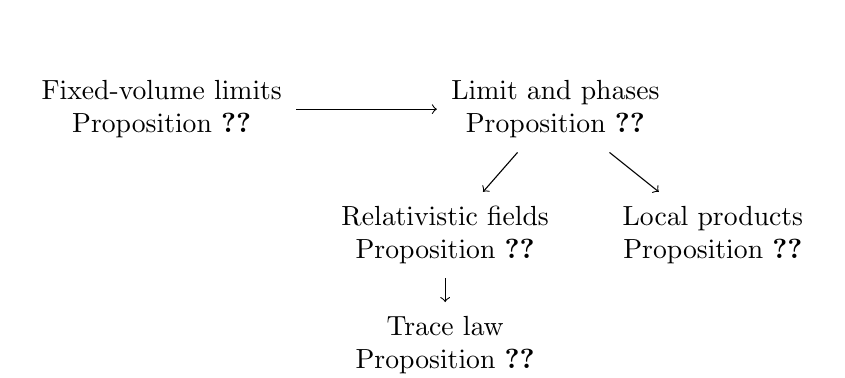
\begin{tikzpicture}[every node/.style={align=center,inner sep=5pt}]
\node (uv) at (0,0) {Fixed-volume limits\\Proposition~\ref{prop:uv}};
\node (limit) at (5,0) {Limit and phases\\Proposition~\ref{prop:limit}};
\node (reconstruction) at (3.6,-1.6) {Relativistic fields\\Proposition~\ref{prop:reconstruction}};
\node (ope) at (7,-1.6) {Local products\\Proposition~\ref{prop:ope}};
\node (trace) at (3.6,-3) {Trace law\\Proposition~\ref{prop:trace}};
\draw[->] (uv) -- (limit);
\draw[->] (limit) -- (reconstruction);
\draw[->] (limit) -- (ope);
\draw[->] (reconstruction) -- (trace);
\end{tikzpicture}
\end{center}
Here the last three results all use estimates for the same lattice family and the same continuum hierarchy supplied by the first two.
The arrows show the order of construction, not a claim that compactness alone gives their analytic inputs.

For each gauge group, we make one joint choice of the family in Proposition~\ref{prop:uv}.
For each prescribed increasing volume sequence, we then make one joint choice of a refinement and hierarchy for Propositions~\ref{prop:limit}--\ref{prop:trace}.
Their conclusions are not asserted for an arbitrary regular family or an arbitrary smooth table of correlations.
With these common choices, the deduction of Theorem~\ref{thm:main} is just the assembly of the five conclusions; it appears at the end of the next section.

\section{The principal propositions}\label{subsec:principal}

The five propositions below use the joint choices described in Section~\ref{sec:strategy}.
Their complete proofs belong to Part~\ref{part:construction}; the explanations here give the ideas needed to follow the deduction of Theorem~\ref{thm:main}.

\paragraph{Removing the lattice spacing.}
At a fixed physical volume, increasing the number of sites must not change what the model looks like at a fixed larger distance.
The coupling and the normalisation of each observable are chosen to achieve this compatibility.
The first proposition gives both one such choice and convergence along its entire spacing sequence.

\begin{proposition}[Ultraviolet construction]\label{prop:uv}
For every gauge group with simple $\g$ (Definition~\ref{def:gauge}), there exists a regular Wilson family $\W$ (Definitions~\ref{def:family} and~\ref{def:regular}) such that, for every $p,n\in\N$ and $v\in\mathcal T^n$, there exists a smooth kernel $K_{p,v}$ on the periodically separated set of Definition~\ref{def:periodic} with
\begin{equation}\label{eq:fixed-volume}
\lim_{N\to\infty}C_{N,p}(v;f)=\int f(x)K_{p,v}(x)\,dx
\end{equation}
for every separated test $f$ supported inside volume $p$ (Definitions~\ref{def:moments}, \ref{def:tests} and~\ref{def:admissible}).
\end{proposition}

\emph{Idea of the proof.}
Replace the fine link variables by averaged variables at a larger spacing, keeping the integral of the probability density exactly the same.
Where the fields are small, their fluctuations can be compared with a Gaussian integral, whose energy is quadratic.
Where they are large, the energy suppresses their contribution; these configurations are estimated rather than discarded.
Repeating this integration changes the coefficient multiplying the squared curvature.
We account for that change in the coupling, instead of treating it as a small error.
The resulting coupling grows logarithmically as the original spacing shrinks.

We carry the local observables through the same integrations.
Their normalisation is fixed at a reference scale, so different cutoffs are compared there rather than at their different bare couplings.
To prove convergence, stop the integration at an intermediate scale.
At this fixed scale the effective correlations converge with the cutoff, while the remaining error is uniformly small when the intermediate scale is sufficiently fine.
Choosing the intermediate scale first and the cutoffs second proves the Cauchy property.

\gap{The later ultraviolet sections must prove the estimates for integrating small and large fields, identify the change of the actual effective coupling, and establish the fixed-scale Cauchy estimate with a uniformly small remaining error.
The fixed-volume conclusion has been checked in the formal source; its analytic proof is still missing from this manuscript.\sourcefootnote{\nolinkurl{Construction.lean}, lines 15--40; \nolinkurl{HierarchyBridge.lean}, lines 16--26; \nolinkurl{YM/FullVolume/Profiles.lean}, lines 25--47.}}

\paragraph{Enlarging the volume and separating phases.}
The estimates for a fixed collection of observables must remain bounded when the surrounding box grows.
They give compactness, but the limit can retain several possible vacuum states.
The next proposition includes the separate argument that resolves this average into phases.

\begin{proposition}[Continuum limit and phases]\label{prop:limit}
For the jointly chosen family of Proposition~\ref{prop:uv} and every strictly increasing $p:\N\to\N$, there exist a strictly increasing $q:\N\to\N$ and hierarchy data (Definition~\ref{def:hierarchy}) satisfying the limit~\ref{main:1} and the phase and regularity conditions~\ref{recon:7}--\ref{recon:12} of Definition~\ref{def:reconstructed}.
\end{proposition}

\emph{Idea of the proof.}
Reflection positivity bounds an average of several separated observables by averages of reflected copies of each individual observable.
The ultraviolet estimates bound these individual averages independently of box size.
Integrating between successive lattice slices controls changes in the correlations when their points move, as explained in Subsection~\ref{subsec:iv-compactness}.
Uniform bounds on the values and on these changes allow a subsequence to be selected for all polynomial basis tuples and all compact sets at once (Lemma~\ref{lem:uv-labels}).
Lattice summation by parts relates derivatives of the limits to insertions of higher degree and gives smoothness.
The fixed-volume limits of Proposition~\ref{prop:uv} identify every inner limit, so only the volume subsequence remains to be chosen.

The average state is split into phases by examining observables separated by a very long time.
In the Hilbert space obtained from reflection positivity, long-time evolution removes the positive-energy part and retains the zero-energy vectors.
Observables placed between these long evolutions act on that zero-energy space.
Once rotations are established, exchanging a time direction with a spatial direction shows that these limiting operators commute.
Representing these commuting operators by continuous functions gives the compact phase space; their vacuum expectations give its probability measure.
This produces the mixture identity~\eqref{eq:mixture}.

\gap{The infinite-volume argument still needs the same-family bounds for local observables and their derivative representatives from the ultraviolet sections.
The later symmetry and phase sections must also prove that the contribution from a far-away stress integral tends to zero and that the long-time operators commute; neither follows from compactness alone.\sourcefootnote{\nolinkurl{YM/Extraction/Limits.lean}, lines 26--43; \nolinkurl{HierarchyBridge.lean}, lines 44--57 and 82--119; the phase representation is in \nolinkurl{YM/Phase/Mixture.lean}.}}

\paragraph{Recovering relativistic fields.}
Euclidean time evolution damps positive energies.
Allowing time to become complex relates this damping to unitary time evolution, and hence to relativistic vacuum expectations.
The estimates must hold as the imaginary time separations tend to zero, because the resulting fields are distributions.

\begin{proposition}[Relativistic reconstruction]\label{prop:reconstruction}
For the jointly chosen hierarchy of Proposition~\ref{prop:limit}, the selected theory satisfies~\ref{recon:1}--\ref{recon:6} and the continuation satisfies~\ref{recon:13}--\ref{recon:15} of Definition~\ref{def:reconstructed}, with the same fields and phase as in Definition~\ref{def:hierarchy}.
\end{proposition}

\emph{Idea of the proof.}
First place Euclidean observables in thin, separated time intervals.
Their bounds show that the continued correlations have distributional limits when the imaginary time separations disappear.
Positivity turns these limits into inner products of field words applied to the vacuum, with words as in~\eqref{eq:domain}.
Completing this space gives the Hilbert space, and multiplication by one more smeared field defines its operator action.

Rotation identities continue to Lorentz transformations.
Together with positivity of Euclidean energy, this confines energy and momentum to the forward cone.
To prove locality, compare the two orders of neighbouring fields at spacelike separated points: their analytic continuations agree on the Euclidean configurations and therefore give the same boundary values there.
The quotient in Proposition~\ref{prop:iv-smooth} removes classical polynomials whose correlations all vanish; the phase construction retains these null relations.
This gives faithful field labels in the sense of~\ref{recon:2}, while the constant observable $1$ supplies a nonzero field.

\gap{The reconstruction section must prove the bounds as imaginary time separations vanish and justify the equality of the two analytic orderings at spacelike separation.
The exact selected-phase and product-test conclusions have been checked in the formal source; these analytic arguments remain unwritten.\sourcefootnote{\nolinkurl{PublicTheory.lean}, lines 93--319; \nolinkurl{HierarchyBridge.lean}, lines 82--133; boundary and locality proofs are organised in \nolinkurl{YM/Work/C01.lean} through \nolinkurl{C29.lean}.}}

\paragraph{Replacing a cluster by a single field.}
A distant observation cannot resolve every detail of several nearby insertions.
The operator product expansion expresses their effect through a finite list of fields at the cluster centre.
The coefficients must be independent of which distant observations are subsequently made.

\begin{proposition}[Common operator product expansion]\label{prop:ope}
The fields and coefficients in~\ref{hierarchy:7} of the jointly chosen hierarchy satisfy~\ref{ope:1}--\ref{ope:2} of Definition~\ref{def:ope}, for the clusters of Definition~\ref{def:cluster}.
\end{proposition}

\emph{Idea of the proof.}
Average the clustered observables from their separation scale toward a larger scale, keeping track of which single local fields they produce.
Retain the terms through degree $D$ and estimate everything else.
The first omitted degree gives the power $D+1$ in the remainder.
The arbitrarily small loss in that power accommodates logarithmic factors.
A fixed collection of correlations with distant test fields determines the coefficients once, before any later spectator fields or phase are chosen.
The error has an operator-norm bound before these commuting operators are evaluated in a phase, so the same bound holds in every phase and in the average state.

\gap{The product section must prove the local-product remainder estimate and show how the fixed coefficient choice gives an operator bound before evaluation in a phase.
The quantifiers and both powers of the radius in~\ref{ope:1}--\ref{ope:2} have been checked; their analytic proof is still deferred.\sourcefootnote{\nolinkurl{ChallengeSpec.lean}, lines 58--80; \nolinkurl{HierarchyBridge.lean}, lines 68--80; \nolinkurl{YM/OPE/Orbits/Kernel.lean}, lines 62--77.}}

\paragraph{Detecting the logarithmic correction.}
The construction supplies a stress tensor and subtracts the selected vacuum expectation from its trace.
Comparison at short distances identifies the leading two-point singularity of this centred field.
The logarithmic correction to that singularity is incompatible with the finite free-field expressions in Definition~\ref{def:wick}.

\begin{proposition}[Trace law and finite-profile exclusion]\label{prop:trace}
The field $\Theta\in F_4$ of the jointly chosen hierarchy satisfies~\ref{trace:1}--\ref{trace:4} of Definition~\ref{def:trace} in the theory of Proposition~\ref{prop:reconstruction}, with the two-point function of Definition~\ref{def:trace-pair}.
\end{proposition}

\emph{Idea of the proof.}
At small distances the fields can be compared, after adjusting their normalisations, with the free Maxwell fields of Section~\ref{sec:maxwell}.
The trace carries an additional inverse running coupling at each insertion.
Since that coupling grows logarithmically, its two-point function acquires the inverse square logarithm in~\eqref{eq:trace-law}.
The coefficient of the logarithmic growth enters both the running coupling and the trace normalisation, and cancels from their ratio.
The final amplitude by itself therefore does not check that coefficient.

The comparison initially works at specially chosen scales.
The positive-energy spectral representation expresses the two-point function through decaying exponentials of the time separation with positive weights.
It therefore decreases with separation, so its values just above and below a requested separation bound its value there.
Every sequence of radii approaching zero has a subsequence where the comparison applies; thus a sequence contradicting the full limit cannot exist.
Finite Wick profiles instead have expansions in integer powers of $r$ and nonnegative powers of $\log r$.
Such expansions cannot have the positive inverse-logarithmic behaviour in~\eqref{eq:trace-law}.

\gap{The trace section must prove the stress normalisation, comparison along subsequences of arbitrary radii, the spectral comparison between nearby separations, and the small-radius expansions of the finite comparison kernels~\eqref{eq:mode}.
The amplitude and the exact finite comparison class have been checked; these proofs remain to be supplied.\sourcefootnote{\nolinkurl{TraceBridge.lean}, lines 14--44; \nolinkurl{YM/TraceExtension/Verse/Cape.lean}, lines 53--88; \nolinkurl{YM/TraceExtension/Wick/Log.lean}, lines 96--108.}}

\begin{proof}[Deduction of Theorem~\ref{thm:main} from the principal propositions]
Fix the gauge group and choose the family of Proposition~\ref{prop:uv}, including its insertions and positive regularity slope.
For a prescribed strictly increasing $p$, take the common $q$ and hierarchy of Proposition~\ref{prop:limit}.
This gives~\ref{main:1} and~\ref{recon:7}--\ref{recon:12} on that refinement.
Proposition~\ref{prop:reconstruction} supplies the remaining reconstruction properties, hence~\ref{main:2}.
Propositions~\ref{prop:ope} and~\ref{prop:trace} give~\ref{main:3} and~\ref{main:4} for those same objects.
\end{proof}


\section{The constants and the order of their choice}\label{sec:constants}

The construction requires each scale to be large enough for estimates whose constants were fixed earlier. This section explains that order. It first separates the positive penalty chosen before the Wilson family from the later numerical choices inside the construction. It then records how the block ratios pay for those choices and how the coupling trajectory is selected. The resulting order matches the family-before-volume choice in Theorem~\ref{thm:main} and Proposition~\ref{prop:uv}.

\paragraph{The public choice.}
Fix a gauge group with simple Lie algebra and choose a penalty $b>0$. The construction then chooses one Wilson family $\W$ with that penalty. Only after the family is fixed does one prescribe an increasing volume sequence; for that sequence, Proposition~\ref{prop:limit} chooses a common refinement and hierarchy. Thus the penalty and family are independent of the later volume sequence, while the refinement and continuum data may depend on it.\sourcefootnote{`YM/Nonperturbative/Headlines.lean`, theorem `existence`; `YM/Nonperturbative/Continuum.lean`, theorem \nolinkurl{continuum_with_position_tests}; `Construction.lean`, theorem `constructed`.}

\paragraph{Choices made before the block ratios.}
At each regularity index, the construction first fixes the data that a later block must accommodate: a kernel with the prescribed penalty, a starting index, and a stage profile. The profile sets the work required at that index: derivative order and spatial power govern the correlation estimates, support exponent and width govern the local terms, path count and column bound control how many terms are carried, and the clip relaxation and drift allowance limit losses at one step. Write $\omega_j$ for the drift allowance at index $j$. The one-loop error bound is fixed at this stage as well. These data describe the accuracy and cost required at each level; they are chosen before any block ratio is selected.\sourcefootnote{`YM/Price/Intent.lean`, structures `Sheet` and `Stage`; `outline/notes/III-2.md`, order of choices.}

\paragraph{Block ratios and later thresholds.}
Next choose one nondecreasing sequence of odd block factors large enough to meet every earlier stage requirement. To specify the stage cost, let $\varpi_j$ be the path count, $w_j$ the width, $\gamma_j$ the column bound, $r_j$ the clip relaxation and $a_j$ the support exponent in the profile, and set
\begin{equation}\label{eq:constants-stage-cost}
 \mathcal C_j=1+\varpi_j+w_j^{-1}+\gamma_j+r_j+a_j\,.
\end{equation}
The factors are chosen so that, at each sufficiently large index $j$,
\begin{equation*}
 \frac{\omega_j}{\log\ell_j}\leq\min\left(\frac{\kappa}{4},j^{-2}\right),\qquad
 \frac{\log\mathcal C_j}{\log\ell_j}\leq j^{-2}\,.
\end{equation*}
Thus each step's allowed coupling drift and the logarithmic cost of the stage data are small compared with the logarithmic increase in lattice size. The smallness exponents then limit errors in the post-block estimates; post-block costs record the further bounds those estimates must pay. Entry thresholds specify how large the reference coupling and accumulated scale must be before a stage is used. Volume conditions require the torus to contain the stage's patches and comparison regions. After choosing these quantities, choose the barrier $\bar\beta$, which supplies the initial coupling and may exceed any prescribed lower bound. Finally choose waiting windows, which keep a fixed regularity index available long enough for its comparisons, and a minimum period length for the tori.\sourcefootnote{`YM/Price/Intent.lean`, `Rolls`, `Protection`, `Delays`, `Bar` and `Wait`; `YM/Price/Length.lean`, theorem \nolinkurl{Bar.exists_above}.}

\paragraph{One schedule for every cutoff.}
After these data are fixed, assign the regularity indices $J_m$ to the successive scales. The sequence is nondecreasing, increases by at most one at each step, and tends to infinity. Let $\kappa>0$ be the group-dependent one-loop slope in~\ref{reg:1}. The scale and block ratio at step $m$ are
\begin{equation}\label{eq:constants-schedule}
 s_m=\sum_{i=0}^{m-1}\log L_i,\qquad L_m=\ell_{J_{m+1}},\qquad
 \widehat\beta_m=\bar\beta+\kappa s_m\,.
\end{equation}
Here $s_m$ is the accumulated logarithmic change of lattice size (with $s_0=0$), and $\widehat\beta_m$ is the reference coupling at that scale. The same sequence $(L_m)$ is used for every cutoff and volume. The schedule makes $\omega_{J_{m+1}}/\log L_m$ tend to zero; since $J_m$ tends to infinity, the accumulated drift is $o(s_m)$.

For fixed cutoff $N$ and volume index $p$, the shooting argument selects effective couplings $\beta_{N,p,m}$ along the scales, starting at the barrier and obeying
\begin{equation*}
 \beta_{N,p,0}=\bar\beta,\qquad
 \left|\beta_{N,p,m+1}-\beta_{N,p,m}-\kappa\log L_m\right|
 \leq \omega_{J_{m+1}}\,.
\end{equation*}
Summing the one-step drift and using the common initial value gives
\begin{equation*}
 \left|\beta_{N,p,m}-\widehat\beta_m\right|
 \leq \sum_{i=0}^{m-1}\omega_{J_{i+1}}\,.
\end{equation*}
For every $\varepsilon>0$, the factor choice makes $\omega_{J_{i+1}}\leq\varepsilon\log L_i$ for all sufficiently large $i$, since $J_i\to\infty$. The finitely many earlier drift allowances have a fixed sum, and $s_m\to\infty$. Dividing the sum by $s_m=\sum_{i<m}\log L_i$ therefore gives $o(1)$. The bound is uniform in $N\geq m$ and $p$, because each one-step drift bound is uniform in those indices. Hence $\beta_{N,p,m}-\widehat\beta_m=o(s_m)$ as $m\to\infty$, uniformly in $N\geq m$ and $p$. This is the running-coupling estimate used in Definition~\ref{def:regular}. It records an order of construction, not numerical values for the intermediate constants.\sourcefootnote{`YM/Lattice/Scale.lean`, `Schedule.scale`; `YM/RG/History.lean`, `Calendar.hatBeta`; `YM/Price/Intent.lean`, `Selected`; `YM/Shoot/Race.lean`, theorem `Recipe.races`.}

\clearpage
\part{The construction}\label{part:construction}
\phantomsection\label{sec:construction-guide}

Part~\ref{part:main} states what the limiting theory must satisfy.
Here we explain how to construct it from the Wilson measure of Definition~\ref{def:wilson-law}.
The construction first removes the spacing at each fixed volume, then takes a subsequence as the volume grows. The later sections explain how those limiting correlations define fields, symmetries and phases.

\paragraph{Following an observable across scales.}
Section~\ref{sec:uv-lattice} starts with the finite probability law and its exact symmetries.
It describes a classical local observable by a gauge-invariant polynomial in the Taylor coefficients of a smooth connection (Definition~\ref{def:uv-labels}); the connection specifies infinitesimal parallel transport, and these coefficients record its behaviour near one point.
A polynomial in nearby link matrices represents that classical polynomial on the lattice.
Integrating out fine links can change its coefficients, so Definition~\ref{def:observables} gives it a fixed index and~\eqref{eq:uv-insertion} fixes the coefficients at a reference level.
This lets us follow one observable through different lattice spacings.

Section~\ref{sec:uv-activities} constructs the link polynomials and organises products of insertions for integration.
It records each contribution together with the lattice region on which it depends; terms where a plaquette is far from the identity are kept and tracked by their sites.
This bookkeeping prepares the estimates but does not prove them.

The later ultraviolet sections perform these integrations one spacing at a time.
They average over finer link variables to produce a density for the remaining coarse links, preserving the original integral.
The estimates must control both this density and each insertion after many such steps.
When every plaquette matrix in a region is close to the identity, the Wilson energy is compared with its quadratic approximation.
When a plaquette is farther away, its contribution is bounded using the energy instead of being discarded.
Contributions are grouped by the sites on which they depend, which is what allows bounds for one local observable to be independent of the surrounding box.
The change in the coefficient of the quadratic curvature term is included in the coupling assigned to the original lattice measure.

These arguments must provide two kinds of estimates.
At a fixed box size, they must show that correlations approach a limit along the full sequence of spacings, as in Proposition~\ref{prop:uv}.
Uniform bounds on local observables and on their finite differences as an insertion point moves must also hold independently of box size.
The latter bounds give a convergent subsequence as the box grows; the fixed-volume limits identify its inner limits with those of the full spacing sequence.
For the moments of Definition~\ref{def:moments}, the intended passage is the ordered limit~\eqref{eq:ordered}:
\begin{equation*}
\begin{aligned}
 C_{N,p}(v;f)&\longrightarrow R_p &&(N\to\infty,\ p\text{ fixed}),\\
 R_{p(q(k))}&\longrightarrow\int f(x)S^\mix(\pi(v_1),\ldots,\pi(v_n);x)\,dx
 &&(k\to\infty).
\end{aligned}
\end{equation*}
Here $f$ is a separated test of Definition~\ref{def:tests}; the inner limit is required at every volume containing its support (Definition~\ref{def:admissible}).
The family is chosen before the prescribed volume sequence $p$, and the subsequence $q$ is the same for every observable list and test.

\paragraph{From correlation functions to fields.}
Section~\ref{sec:infinite-volume} applies reflection positivity: for positive-time products $F,G$, reflect $F$ across time zero and take its complex conjugate, writing the result as $\vartheta F$.
The resulting positive form is $S^{\mix}((\vartheta F)G)\ge0$; the finite-lattice inequality is~\eqref{eq:iv-lattice-rp}, and its repeated-cell version is~\eqref{eq:iv-chessboard}.
Repeated reflection bounds a joint correlation by one-cell bounds, which do not grow with the box.
These bounds give one subsequence for all correlations.
To identify derivatives, the proof compares a finite difference of an insertion's position with a higher-degree observable.
Two observables are identified as the same continuum field when every tested limiting correlation of their difference is zero; removing this null subspace gives the field spaces of the limit.
Smoothness therefore needs estimates for these comparisons, not just compactness.
Finally the fixed-volume theorem removes the temporary spacing subsequence and gives the ordered limit of Definition~\ref{def:ordered}.

Section~\ref{sec:maxwell} compares the limiting fields at short distances with the explicit curvature fields of the free Maxwell theory.
These are the field strengths of a free electromagnetic field; finite tests distinguish the field classes, and comparison maps transfer the stress-tensor estimates to the interacting theory.
Constructing these maps requires short-distance bounds and a separate dimension bound.
The comparison does not make the interacting theory free.
For the symmetry argument, the stress-tensor integral identities are a separate required input to establish continuous rotations on this space; they are not proved in the sections presented here.

\paragraph{Reading the construction.}
When reading an estimate, identify the quantities held fixed, the limit being taken, and whether its bound depends on volume.
This is especially important when a fixed-volume spacing limit is used inside the later volume subsequence.


\section{Lattice fields}\label{sec:uv-lattice}

The field at a point will be represented by observables on finitely many nearby links.
There are two choices to make: which classical field an observable represents, and how to change its coefficients as the lattice spacing decreases.
This section specifies these choices without yet integrating out any scales.

We begin with the exact symmetries of the Wilson measure in Subsection~\ref{subsec:uv-law}.
Subsection~\ref{subsec:uv-labels} describes classical local fields by their Taylor coefficients and chooses finite bases of polynomial labels.
Subsection~\ref{subsec:uv-local} states how a polynomial in link matrices must reproduce those labels.
Subsection~\ref{subsec:uv-renormalized} then gives the reference-scale normalization of the lattice insertions.
Section~\ref{sec:uv-activities} constructs the local polynomials and introduces the activity sums used in the integration argument; the coefficient transfers require the later renormalization steps.

We use the lattice, plaquettes and measure of Definitions~\ref{def:lattice}, \ref{def:plaquette} and~\ref{def:wilson-law}.
The gauge group is as in Definition~\ref{def:gauge}; simplicity and connectedness are not needed in this section.

\subsection{The Wilson measure}\label{subsec:uv-law}

The action depends on the transport around each elementary square, or plaquette, as explained in Definition~\ref{def:plaquette}.
Conjugating that transport or reversing its direction leaves the action unchanged.
This observation gives exact symmetries of the probability measure, before any limit is taken.

Write~$U(w)$ for the ordered transport along a walk~$w$ from~$x$ to~$z$, using the link convention of Definition~\ref{def:lattice}.
The gauge action of Definition~\ref{def:gauge-transform} gives
\begin{equation}\label{eq:uv-gauge}
 U^\gamma(w)=\gamma(x)U(w)\gamma(z)^{-1}\,.
\end{equation}
The factors at intermediate vertices cancel, for forward and backward steps alike.
For the estimates below, abbreviate the single-plaquette action and define its associated distance from the identity by
\begin{equation}\label{eq:uv-chord}
 s(u)=1-\frac{1}{m}\operatorname{Re}\tr u,
 \qquad \chi(u)=\frac{\|u-1\|_{\mathrm F}}{\sqrt m}\qquad(u\in G),
\end{equation}
where~$\|\cdot\|_{\mathrm F}$ is the Frobenius norm.
Unitarity gives
\begin{equation}\label{eq:uv-chord-square}
 \chi(u)^2=2s(u),\qquad 0\le s(u)\le2,\qquad
 \chi(uv)\le\chi(u)+\chi(v)\,.
\end{equation}
Indeed, $\|u-1\|_{\mathrm F}^2=2m-2\operatorname{Re}\tr u$ and~$\|u-1\|_{\mathrm F}\le2\sqrt m$.
For the last inequality, write~$uv-1=(u-1)+u(v-1)$ and use invariance of the Frobenius norm under unitary multiplication.
Both~$s$ and~$\chi$ are continuous and invariant under conjugation and inversion.

The coordinate symmetries we use are the permutations and reversals of the four lattice axes.
They act on link configurations by transporting each link along its image.

\begin{definition}[Coordinate symmetries]\label{def:uv-symmetries}
Let~$H_4$ be the group of signed permutation matrices.
For~$A(y)=hy+z$, with~$h\in H_4$ and~$z\in\Lambda_\ell$, the pullback~$A^*U$ reads the transport along the image of each positive link.
A reversed image uses the inverse variable, with its initial vertex shifted accordingly.
The lattice and link conventions are those of Definition~\ref{def:lattice}.
\end{definition}

Write~$\mathcal U_\ell$ for the configuration space of Definition~\ref{def:lattice}, and~$B_b(\mathcal U_\ell;\C)$ for its bounded Borel complex functions.
The following proposition justifies ordinary expectations of local polynomials and the changes of variables used throughout the construction.

\begin{proposition}[The lattice law]\label{prop:uv-law}
For~$\ell\ge1$ and~$\beta\in\R$, the measure of Definition~\ref{def:wilson-law} satisfies
\begin{equation}\label{eq:uv-law}
 \mu_{\ell,\beta}(\mathcal U_\ell)=1,\qquad
 C(\mathcal U_\ell;\C)\cup B_b(\mathcal U_\ell;\C)
 \subseteq L^1(\mu_{\ell,\beta})\,.
\end{equation}
For every gauge transformation~$\gamma$ of Definition~\ref{def:gauge-transform}, coordinate symmetry~$A$ of Definition~\ref{def:uv-symmetries}, and~$F\in L^1(\mu_{\ell,\beta})$,
\begin{equation}\label{eq:uv-expectation-symmetry}
 \int F(U^\gamma)\,d\mu_{\ell,\beta}(U)
 =\int F(U)\,d\mu_{\ell,\beta}(U)
 =\int F(A^*U)\,d\mu_{\ell,\beta}(U)\,.
\end{equation}
\end{proposition}

\begin{proof}
We preserve the reference product measure and the energy separately.
Each transformation therefore preserves the Wilson measure.
Write~$\eta_\ell$ for the product Haar measure in~\eqref{eq:wilson-law}.

The closed group~$G\subset U(m)$ and its finite configuration space are compact.
There are six plaquettes per site, each with energy in~$[0,2]$.
Thus
\begin{equation}\label{eq:uv-density-bounds}
 0\le E_\ell\le12\ell^4,\qquad
 e^{-12|\beta|\ell^4}\le e^{-\beta E_\ell(U)}\le e^{12|\beta|\ell^4}\,.
\end{equation}
Integrating against probability Haar gives a finite positive normalizer.
A continuous function on the configuration space is bounded, so both classes in~\eqref{eq:uv-law} are integrable.

Haar invariance allows a fixed matrix to be multiplied on either side of a link, and allows its orientation to be reversed.
For~$R_g(u)=ug$, $\mathrm{inv}(u)=u^{-1}$ and every integrable~$f:G\to\C$, the identities are
\begin{equation}\label{eq:uv-haar-changes}
 (R_g)_*h=h,\qquad \mathrm{inv}_*h=h,\qquad
 \int_G f(aub)\,h(du)=\int_G f(u)\,h(du)\quad(a,b\in G)\,.
\end{equation}
Indeed, $(R_g)_*h$ is left invariant with mass one, so Haar uniqueness identifies it with~$h$.
The image under inversion is then left invariant by right invariance of~$h$, again with mass one.
Applying these identities independently to each link gives, for the gauge map~$\Gamma_\gamma:U\mapsto U^\gamma$,
\begin{equation}\label{eq:uv-product-changes}
 (\Gamma_\gamma)_*\eta_\ell=\eta_\ell,\qquad
 (A^*)_*\eta_\ell=\eta_\ell\,.
\end{equation}
For the second identity, the coordinate symmetry permutes the positive links and inverts those whose image orientation is negative.

It remains to check the energy.
By~\eqref{eq:uv-gauge}, a gauge transformation conjugates a plaquette transport at its initial vertex.
A coordinate symmetry sends an elementary square to another one, up to a change of initial corner and orientation.
To check the counting, write~$he_\mu=\sigma_\mu e_{\pi(\mu)}$, with~$\sigma_\mu\in\{-1,1\}$.
The positive-axis base of the image square is
\begin{equation*}
 hy+z-\mathbf1_{\{\sigma_\mu=-1\}}e_{\pi(\mu)}
      -\mathbf1_{\{\sigma_\nu=-1\}}e_{\pi(\nu)},
\end{equation*}
and its axis pair is the increasing rearrangement of~$\{\pi(\mu),\pi(\nu)\}$.
This permutes the face indices even when~$\ell=1$ or~$2$.
Since conjugation and inversion preserve~$s$, we have
\begin{equation}\label{eq:uv-energy-invariance}
 E_\ell(U^\gamma)=E_\ell(U),\qquad E_\ell(A^*U)=E_\ell(U)\,.
\end{equation}
For either~$T=\Gamma_\gamma$ or~$T=A^*$, equations~\eqref{eq:uv-product-changes} and~\eqref{eq:uv-energy-invariance} now give
\begin{equation*}
 \int F(TU)\,d\mu_{\ell,\beta}(U)
 =\frac{1}{Z_{\ell,\beta}}\int F(TU)e^{-\beta E_\ell(TU)}\,d\eta_\ell(U)
 =\int F(U)\,d\mu_{\ell,\beta}(U)\,.
\end{equation*}
This proves~\eqref{eq:uv-expectation-symmetry} for every integrable~$F$.
\end{proof}

\subsection{Classical labels}\label{subsec:uv-labels}

We now choose concrete classical quantities for the lattice observable labels of Definition~\ref{def:observables}.
A connection near the origin is described in radial gauge: its component in the radial direction vanishes.
Its Taylor coefficients then satisfy a linear constraint, degree by degree.
The constant coefficient vanishes: a constant one-form with zero contraction against every radial vector must be zero.
A polynomial in finitely many such coefficients describes a classical local observable; invariance under simultaneous conjugation removes the choice of gauge at the origin.

\begin{definition}[Classical labels]\label{def:uv-labels}
For~$\g$ of Definition~\ref{def:gauge} and~$j\ge0$, let~$\mathcal A_j$ be the real space of homogeneous polynomial one-forms of degree~$j+1$, with values in~$\g$, satisfying
\begin{equation}\label{eq:uv-radial}
 \sum_{\mu=1}^4 z^\mu A_{j,\mu}(z)=0\qquad(z\in\R^4)\,.
\end{equation}
The list of Taylor coefficients, called a real jet, is a sequence~$J=(A_j)_{j\ge0}$ with~$A_j\in\mathcal A_j$.
Choose real coordinates on each~$\mathcal A_j$, assigning weight~$j+2$ to each coordinate.
Let~$V_d$ be the space of complex polynomials in these coordinates, of total weight at most~$d$, invariant under simultaneous conjugation by~$G$.
\end{definition}

The coefficients in Definition~\ref{def:uv-labels} are Taylor coefficients, with the factorial normalization, rather than derivative values.
Equivalently, they are diagonal evaluations of symmetric~$(j+1)$-linear maps.
The weight~$j+2$ records the scaling of a link integral: the polynomial one-form contributes~$j+1$ powers of length and integration contributes one more.
Weights add under multiplication.
We also count the number of factors in a monomial, its ordinary polynomial degree; the two gradings will serve different purposes.

An orthogonal matrix~$h$ acts on these one-forms and on their invariant polynomials by
\begin{equation}\label{eq:uv-label-action}
 (T_hA_j)_\mu(z)=\sum_\nu h_{\mu\nu}A_{j,\nu}(h^{-1}z),
 \qquad (h\cdot v)(J)=v(T_{h^{-1}}J)\,.
\end{equation}
This action preserves~\eqref{eq:uv-radial} and commutes with conjugation by~$G$.
Coefficient conjugation is denoted by~$v\mapsto\bar v$; a real polynomial has~$\bar v=v$.
Let~$V_d^{w,f}$ be the subspace homogeneous of weight~$w$ and factor number~$f$.

The weight bound leaves only finitely many coordinates and monomials.
We can therefore choose one finite basis at each degree, retaining the basis elements already chosen at lower degrees.
Real homogeneous bases make conjugation and the two gradings explicit.

\begin{lemma}[Finite label spaces]\label{lem:uv-labels}
For the spaces of Definition~\ref{def:uv-labels}, evaluation on real jets is injective, and
\begin{equation}\label{eq:uv-label-grading}
 \dim_\C V_d<\infty,\qquad 1\in V_d\subseteq V_{d+1},\qquad
 V_d=\bigoplus_{\substack{0\le w\le d\\0\le f\le w}}V_d^{w,f}\,.
\end{equation}
Each summand is preserved by~\eqref{eq:uv-label-action} and coefficient conjugation.
There are nested real bases, homogeneous in both gradings and containing~$1$.
\end{lemma}

\begin{proof}
The weight bound reduces the problem to finitely many monomials; we then choose bases separately in their real homogeneous components.

Only coordinates with~$j+2\le d$ can occur in a monomial of weight at most~$d$.
There are finitely many such coordinates, and the exponent of each is bounded by~$d$.
Thus finitely many monomials span the polynomials under consideration, and their invariant subspace is finite dimensional.
A complex polynomial vanishing on every real jet vanishes identically, by the one-variable polynomial identity theorem applied successively in these finitely many real coordinates.

Conjugation acts linearly within each~$\mathcal A_j$ and therefore preserves both grades.
Writing~$v=\sum_{w,f}v^{w,f}$, comparison of the homogeneous terms gives
\begin{equation}\label{eq:uv-homogeneous-invariance}
 v(\Ad(g)J)=v(J) \Longrightarrow\quad
 v^{w,f}(\Ad(g)J)=v^{w,f}(J)\qquad(g\in G)\,.
\end{equation}
Thus the homogeneous parts of an invariant polynomial are themselves invariant.
Every coordinate has weight at least two; in particular the factor number cannot exceed the weight, giving the index range in~\eqref{eq:uv-label-grading}.
The same linearity argument applies to~\eqref{eq:uv-label-action}, and these real linear changes commute with coefficient conjugation.
Each invariant homogeneous component is the complex span of its real polynomials, by decomposition into real and imaginary coefficient parts.
Choose a real basis in each component, beginning with~$\{1\}$ for the constant component, and retain these choices as~$d$ increases.
\end{proof}

Fix the bases of Lemma~\ref{lem:uv-labels}, writing~$b_{d,i}$ for their elements and~$(w_{d,i},f_{d,i})$ for their two grades, with~$b_{d,0}=1$.
We identify each polynomial with its coefficient vector when applying a linear map to~$V_d$.
The continuum spaces~$F_d$ of Definition~\ref{def:hierarchy} will arise only after a limiting correlation table and its null relations have been obtained.
The spaces~$V_d$ still contain all classical labels, before these relations are imposed.

\subsection{Local representatives}\label{subsec:uv-local}

A polynomial in Taylor coefficients is not yet a lattice observable.
We seek a polynomial in nearby link matrices whose Taylor expansion, when tested on a classical connection, recovers the chosen label.
This is the purpose of a local section.
Its existence is a separate construction; here we state its normalization precisely.

On~$\Z^4$, the gauge action of Definition~\ref{def:gauge-transform} and the coordinate pullbacks of Definition~\ref{def:uv-symmetries} use the same formulas as on a torus.
Polynomial functions on a finite set of links can then be evaluated on any periodic lattice.

\begin{definition}[Local polynomial functions]\label{def:uv-polynomials}
For a finite set~$\Sigma\subset\Z^4$, let~$\mathcal P(\Sigma)$ be the polynomial functions of matrix entries and conjugate entries of links with both endpoints in~$\Sigma$.
At~$o\in\Lambda_\ell$, evaluate such a polynomial by substituting
\begin{equation}\label{eq:uv-placement}
 U(x,\mu)\longmapsto U(o+[x]_\ell,\mu)\,.
\end{equation}
The link conventions are those of Definition~\ref{def:lattice}.
\end{definition}

This implements the finite-site locality requirement~\ref{reg:4} of Definition~\ref{def:regular}.
The substitution is meaningful even when distinct cover links become the same torus link.

To test the classical normalization, truncate a real jet of Definition~\ref{def:uv-labels} to weights at most~$d$ and set~$A^J_\mu=\sum_{j+2\le d}A_{j,\mu}$.
We obtain the test links by solving a matrix equation, and then use closedness of~$G$ to see that the solution remains in the group.
For a spacing parameter~$\varepsilon\in\R$, put
\begin{equation}\label{eq:uv-link-ode}
 \begin{aligned}
 B(t)&=\varepsilon A_\mu^J\bigl(\varepsilon(x+te_\mu)\bigr), & u'(t)&=u(t)B(t),\\
 u(0)&=1, & U_{J,\varepsilon}(x,\mu)&=u(1)\,.
 \end{aligned}
\end{equation}
Successive integration gives the ordered series
\begin{equation}\label{eq:uv-transport-series}
 \begin{aligned}
 u(t)&=1+\sum_{r\ge1}\int_{0<s_1<\cdots<s_r<t}
          B(s_1)\cdots B(s_r)\,ds_1\cdots ds_r,\\
 \left\|\int_{0<s_1<\cdots<s_r<t}B(s_1)\cdots B(s_r)\,ds_1\cdots ds_r\right\|_{\mathrm F}
 &\le\frac{M^r}{r!}
 \end{aligned}
\end{equation}
for~$r\ge1$ and~$0\le t\le1$ when~$\|B(s)\|_{\mathrm F}\le M$.
For a fixed real jet, $B$ is polynomial in~$\varepsilon$ and the same factorial majorant holds on a small complex~$\varepsilon$-neighborhood of zero.
The series therefore converges normally there, solves the equation, and gives an endpoint real analytic in~$\varepsilon$ near zero.
Iterating the integral equation for the difference of two solutions gives the same factorial bound and proves uniqueness.
For real~$\varepsilon$, step-function approximations to~$B$ have solutions that are products of matrices~$\exp(\Delta t\,B(t_j))\in G$.
The same series bound proves convergence of these products to~$u$; since~$G$ is closed, the links in~\eqref{eq:uv-link-ode} are group valued.

The section must preserve the exact lattice symmetries and the constant observable.
Its classical normalization requires equality of Taylor coefficients through the degree being represented.
These are the conditions in the next definition.

\begin{definition}[Normalized local section]\label{def:uv-sections}
A normalized local section in degree~$d$ is a finite set~$\Sigma_d\subset\Z^4$ and a complex linear map~$P_d:V_d\to\mathcal P(\Sigma_d)$, with polynomial functions as in Definition~\ref{def:uv-polynomials}, such that
\begin{equation}\label{eq:uv-section-support}
 0\in\Sigma_d,\qquad h\Sigma_d=\Sigma_d\quad(h\in H_4),
\end{equation}
and, for all~$v\in V_d$, link configurations~$U$ on~$\Z^4$, $\gamma:\Z^4\to G$ and~$h\in H_4$,
\begin{equation}\label{eq:uv-section-symmetry}
 \begin{aligned}
 P_d[v](U^\gamma)&=P_d[v](U), & P_d[1]&=1,\\
 P_d[\bar v](U)&=\overline{P_d[v](U)}, &
 P_d[v](h^*U)&=P_d[h\cdot v](U)\,.
 \end{aligned}
\end{equation}
For every real jet~$J$ and~$0\le k\le d$, it also satisfies
\begin{equation}\label{eq:uv-section-taylor}
 \left.\frac{d^k}{d\varepsilon^k}P_d[v](U_{J,\varepsilon})\right|_{\varepsilon=0}
 =\left.\frac{d^k}{d\varepsilon^k}v(\operatorname{sc}_\varepsilon J)\right|_{\varepsilon=0},
 \qquad (\operatorname{sc}_\varepsilon J)_j=\varepsilon^{j+2}A_j\,.
\end{equation}
Here~$V_d$, its real jets and its action are as in Definition~\ref{def:uv-labels} and~\eqref{eq:uv-label-action}; $H_4$ and its pullbacks are from Definition~\ref{def:uv-symmetries}, and the test links are~\eqref{eq:uv-link-ode}.
\end{definition}

The Taylor identity imposes no equality at nonzero spacing.
No compatibility of~$P_d$ and~$P_{d+1}$ is required.
Proposition~\ref{prop:uv-sections} constructs these sections and proves the derivative estimates needed for the later blocking argument.

\subsection{Renormalized insertions}\label{subsec:uv-renormalized}

As shorter scales are integrated out, the coefficients of an observable change and different classical labels can mix.
We normalize the observable by its coefficients at one reference level~$r(d)$, chosen independently of cutoff and volume.
The inverse of the coefficient transfer then determines which fine-lattice polynomial represents a prescribed reference label.
This describes a particular choice of the insertions in Definition~\ref{def:observables}, not an additional condition on that definition.

Use~$a_N,N,p$ from Definition~\ref{def:family}, the basis from Lemma~\ref{lem:uv-labels}, and a local section from Definition~\ref{def:uv-sections}.
Let~$\theta_N>0$ be the threshold that will distinguish small plaquette distances~$\chi$ in the later estimates.
Define the linear factor scaling by~$S_t b_{d,i}=t^{f_{d,i}}b_{d,i}$.
For an invertible complex linear map~$\tau_{N,p,d}:V_d\to V_d$, the candidate insertion is
\begin{equation}\label{eq:uv-insertion}
 I_{N,p}\bigl((d,v),o;U\bigr)
 =\frac{1}{a_N^d}P_d\!\left[S_{\theta_N^{-1}}\tau_{N,p,d}^{-1}v\right](o;U),
\end{equation}
with placement~\eqref{eq:uv-placement}.
Thus a label with~$f$ factors is multiplied by~$\frac{1}{\theta_N^f}$; the prefactor~$\frac{1}{a_N^d}$ supplies the physical degree normalization.

For~$N\ge r(d)$, let~$x_j:V_d\to V_d$ be complex linear maps from coefficients at the finest level~$N$ to coefficients at level~$j$, for~$r(d)\le j\le N$.
The conditions that make~$\tau_{N,p,d}$ a reference transfer are
\begin{equation}\label{eq:uv-reference-coordinates}
 x_N(v)=v,\qquad x_{r(d)}(v)=\tau_{N,p,d}v,\qquad
 x_j(a_N^d1)=a_j^d1\quad(r(d)\le j\le N)\,.
\end{equation}
These equalities fix how coefficients are normalized between levels; they assert no pointwise identity between observables on different lattices.
Reality and signed-permutation covariance require
\begin{equation}\label{eq:uv-transfer-symmetry}
 \tau_{N,p,d}\bar v=\overline{\tau_{N,p,d}v},\qquad
 \tau_{N,p,d}(h\cdot v)=h\cdot(\tau_{N,p,d}v)\quad(h\in H_4)\,.
\end{equation}

The locality of the resulting insertion follows from its polynomial formula, even on a torus smaller than the chosen set of sites.
The unit normalization is different: it uses the reference-transfer conditions and therefore applies only beyond the reference level.
The following proposition separates these two conclusions.

\begin{proposition}[Locality of the insertions]\label{prop:uv-insertions}
Let~$P_d$ satisfy Definition~\ref{def:uv-sections}, $\theta_N>0$ and~$\tau_{N,p,d}\in\mathrm{GL}_\C(V_d)$.
For all~$N,p$, the map~$v\mapsto I_{N,p}\bigl((d,v),o;\cdot\bigr)$ in~\eqref{eq:uv-insertion} is complex linear and satisfies~\ref{reg:2}--\ref{reg:4} of Definition~\ref{def:regular}, with finite set~$\Sigma_d$.
Moreover,
\begin{equation}\label{eq:uv-insertion-translation}
 I_{N,p}\bigl((d,v),o;U(\cdot+z)\bigr)=I_{N,p}\bigl((d,v),o+z;U\bigr)\,.
\end{equation}
If~$N\ge r(d)$ and~\eqref{eq:uv-reference-coordinates}--\eqref{eq:uv-transfer-symmetry} hold, then
\begin{equation}\label{eq:uv-insertion-covariance}
 \begin{aligned}
 I_{N,p}\bigl((d,\bar v),o;U\bigr)&=\overline{I_{N,p}\bigl((d,v),o;U\bigr)},\\
 I_{N,p}\bigl((d,h\cdot v),A(o);U\bigr)&=I_{N,p}\bigl((d,v),o;A^*U\bigr),\\
 I_{N,p}\bigl((d,a_{r(d)}^d1),o;U\bigr)&=1,\qquad
 x_{r(d)}(\tau_{N,p,d}^{-1}v)=v
 \end{aligned}
\end{equation}
for~$A(o)=ho+z$, $h\in H_4$, as in Definition~\ref{def:uv-symmetries}.
\end{proposition}

\begin{proof}
Polynomial dependence gives continuity and finite-site locality; the endpoint condition then identifies which label represents the constant observable.

The coefficient changes in~\eqref{eq:uv-insertion} are complex linear.
A polynomial in link entries and their conjugates is continuous, and the section is gauge invariant by~\eqref{eq:uv-section-symmetry}; this proves~\ref{reg:2} and~\ref{reg:3}.
Placement~\eqref{eq:uv-placement} reads only links with both endpoints in~$o+[\Sigma_d]_{L_pD_N}$, proving~\ref{reg:4}.
Identifying distinct cover vertices does not enlarge that set.
Translating the placement proves~\eqref{eq:uv-insertion-translation}.

Factor scaling commutes with coefficient conjugation and~$H_4$, since both actions preserve factor number by Lemma~\ref{lem:uv-labels}.
Together with~\eqref{eq:uv-transfer-symmetry} and~\eqref{eq:uv-section-symmetry}, this gives the first two identities in~\eqref{eq:uv-insertion-covariance}.
For the unit, the endpoint conditions~\eqref{eq:uv-reference-coordinates} give
\begin{equation}\label{eq:uv-unit-calculation}
 \begin{aligned}
 \tau_{N,p,d}^{-1}(a_{r(d)}^d1)&=a_N^d1,\\
 I_{N,p}\bigl((d,a_{r(d)}^d1),o;U\bigr)
 &=\frac{1}{a_N^d}P_d\bigl[S_{\theta_N^{-1}}(a_N^d1)\bigr](o;U)
 =\frac{a_N^d}{a_N^d}P_d[1](o;U)=1\,.
 \end{aligned}
\end{equation}
The remaining identity follows by applying the reference endpoint condition to~$\tau_{N,p,d}^{-1}v$.
\end{proof}

Choose the lattice observable labels in Definition~\ref{def:observables} to be~$\mathcal T=\bigsqcup_dV_d$.
Under the hypotheses of Proposition~\ref{prop:uv-insertions}, the requirements~\ref{reg:2}--\ref{reg:4} are satisfied at every cutoff; the reference unit is~$a_{r(d)}^d1$.
Proposition~\ref{prop:uv-law} makes every lattice moment in~\eqref{eq:smear} an integral of a continuous, hence integrable, product of observables.
The running-coupling condition~\ref{reg:1} and convergence of these moments require the later ultraviolet arguments.

\gap{The invertible coefficient transfers satisfying~\eqref{eq:uv-reference-coordinates}--\eqref{eq:uv-transfer-symmetry} must still be constructed for the same Wilson family. Proposition~\ref{prop:uv-insertions} assumes them. The local sections and their derivative bounds are supplied by Proposition~\ref{prop:uv-sections}; transferring their coefficients through the integration over scales remains a later ultraviolet proof.\sourcefootnote{Transfer conditions: \texttt{YM/Source/Insertion.lean}, lines 89--114; same-family application: \texttt{YM/FullVolume/Cross.lean}, lines 30--71}}

\section{Local polynomials and activities}\label{sec:uv-activities}

Section~\ref{sec:uv-lattice} specified which classical observable a lattice polynomial must reproduce at small spacing.
We now construct those polynomials and introduce the form in which local interactions will be carried through the integration over scales.
The common principle is to retain the region and the coefficients of every term: this allows multiplication and summation without losing the estimates on individual observables.
An activity is a scalar function attached to a finite set of lattice sites, used to represent one term in the weight after some link variables have been integrated out.

Subsection~\ref{subsec:uv-sampling} recovers finitely many Taylor coefficients from finitely many transported plaquettes.
Subsection~\ref{subsec:uv-section-build} turns this recovery into the local representative maps of Definition~\ref{def:uv-sections}, with derivative bounds independent of the torus size.
Subsection~\ref{subsec:uv-markers} records insertions as coefficients of auxiliary commuting variables whose squares vanish.
Subsection~\ref{subsec:uv-activity-format} gives bounds for these activities and proves absolute convergence of their sums.

\subsection{Recovering Taylor coefficients}\label{subsec:uv-sampling}

The curvature of a connection~$A$ is the two-form with components
\begin{equation*}
 F_{\mu\nu}(A)=\partial_\mu A_\nu-\partial_\nu A_\mu+[A_\mu,A_\nu].
\end{equation*}
At first order in the size of~$A$, a plaquette transport records the average of the linear part~$\partial_\mu A_\nu-\partial_\nu A_\mu$ over its square. The commutator term is quadratic, so it does not enter this first variation.
Different squares give different linear measurements of the Taylor coefficients. For any fixed degree, finitely many such measurements suffice; radial gauge makes recovery of the connection from this linear curvature possible.

Fix~$d\in\N$.
Use the spaces~$\mathcal A_j,V_d$ of Definition~\ref{def:uv-labels} and the finite tuples~$J\in\mathcal J_d$ of Definition~\ref{def:uv-test-links}.
Such a tuple specifies the polynomial connection~$A^J$ and the test links~$U_{J,\varepsilon}$ defined there.
On~$\g$ use the norm~$|X|_\g=\frac{\|X\|_{\mathrm F}}{\sqrt m}$, and let~$P_\g$ be real Frobenius orthogonal projection onto~$\g$.
The following matrix-valued function maps a plaquette matrix to the Lie algebra; its derivative at the identity is the identity map, so it retains the linear curvature term just described. Here~$u\in G$, and~$\chi$ is the distance from the identity in~\eqref{eq:uv-chord}:
\begin{equation}\label{eq:uv-curvature}
 \mathcal F(u)=P_\g\!\left(\frac{u-u^{-1}}{2}\right),\qquad
 |\mathcal F(u)|_\g\le\chi(u),\qquad
 \left.\frac{d}{ds}\mathcal F(e^{sX})\right|_{s=0}=X\quad(X\in\g)\,.
\end{equation}
Projection commutes with conjugation by~$G$, since conjugation is orthogonal and preserves~$\g$.
The bound follows by writing~$u-u^{-1}=(u-1)-(u^{-1}-1)$ and using~\eqref{eq:uv-chord-square}.
The derivative follows from~$e^{sX}-e^{-sX}=2sX+O(s^3)$.
Also~$\mathcal F(u^{-1})=-\mathcal F(u)$.

For a plaquette~$p$ based at~$x\in\Z^4$ and a walk~$\omega$ from~$0$ to~$x$, transport its curvature back to the origin:
\begin{equation}\label{eq:uv-transported-curvature}
 Q_{\omega,p}(U)=\Ad\bigl(U(\omega)\bigr)\mathcal F(U_p),\qquad
 Q_{\omega,p}(U^\gamma)=\Ad\bigl(\gamma(0)\bigr)Q_{\omega,p}(U)\,.
\end{equation}
Here~$U(\omega)$ is the ordered walk transport of Definition~\ref{def:uv-walks}, $U_p$ is the plaquette matrix of Definition~\ref{def:plaquette}, and~$\Ad(g)X=gXg^{-1}$ as in Definition~\ref{def:uv-labels}.
The second identity uses the gauge transformation of Definition~\ref{def:gauge-transform} and~\eqref{eq:uv-gauge}.
All these quantities now transform at the same site, so invariant polynomials in them will be gauge invariant.
They read only links in the walk and plaquette, with both endpoints included.

The next lemma supplies a local analytic recovery map.
It uses several plaquettes because their combined measurements have enough independent components to recover all Taylor coefficients through degree~$d$.

\begin{lemma}[Finite sampling]\label{lem:uv-sampling}
There is a finite family~$(\omega_a,p_a)_{a=1}^{M_d}$ for which
\begin{equation}\label{eq:uv-sampler}
 \mathcal Q_d(J)=\bigl(Q_{\omega_a,p_a}(U_{J,1})\bigr)_{a=1}^{M_d},
 \qquad \mathcal Q_d:\mathcal J_d\longrightarrow\g^{M_d},
\end{equation}
has injective derivative at~$0$.
There is a real analytic map~$R_d:\g^{M_d}\to\mathcal J_d$, defined near~$0$, satisfying
\begin{equation}\label{eq:uv-recovery}
 R_d(0)=0,\qquad R_d\mathcal Q_d=\mathrm{id},\qquad
 R_d(\Ad(g)q)=\Ad(g)R_d(q)\quad(g\in G)\,.
\end{equation}
The last two equalities hold near the origin, for each fixed~$g\in G$; the test links are from Definition~\ref{def:uv-test-links}, and~$\Ad(g)$ acts on every component of a tuple.
\end{lemma}

\begin{proof}
The recovery has three steps: all square measurements together detect every jet, finite dimensionality reduces them to finitely many measurements, and the inverse function theorem recovers the jet from their nonlinear values.
The two properties to establish are
\begin{equation*}
 \mathcal Q_d(J)=\bigl(Q_{\omega_a,p_a}(U_{J,1})\bigr)_{a=1}^{M_d},
 \qquad R_d\mathcal Q_d(J)=J\ \text{ near }0.
\end{equation*}

\begin{enumerate}
\item \emph{All square measurements detect the jet.}

Recall that~$A_\mu^J=\sum_{j+2\le d}A_{j,\mu}$ is the truncated connection of Definition~\ref{def:uv-test-links}.
Vary its size by~$\lambda\in\R$ in the transport equation~\eqref{eq:uv-link-ode}, keeping the edge fixed.
At~$\lambda=0$ the solution is~$1$, so its first variation is the integral along that edge:
\begin{equation*}
 \left.\frac{d}{d\lambda}U_{\lambda J,1}(x,\mu)\right|_{\lambda=0}
 =\int_0^1 A_\mu^J(x+te_\mu)\,dt\,.
\end{equation*}
Since~$\mathcal F(1)=0$, differentiating the conjugating transport in~\eqref{eq:uv-transported-curvature} contributes zero.
Consequently, for the unit square~$p=(x;\mu,\nu)$,
\begin{equation}\label{eq:uv-linear-square}
 D\bigl(Q_{\omega,p}(U_{J,1})\bigr)_{J=0}[J]
 =\int_0^1\!\int_0^1
   (\partial_\mu A_\nu^J-\partial_\nu A_\mu^J)(x+se_\mu+te_\nu)\,ds\,dt\,.
\end{equation}
This is independent of~$\omega$.

Suppose all these integrals vanish for integer~$x$.
Each is a polynomial in~$x$; a polynomial vanishing on~$\Z^4$ vanishes everywhere, by successive one-variable polynomial identities.
For the highest homogeneous term~$A_j$, the highest part of that integral is~$\partial_\mu A_{j,\nu}-\partial_\nu A_{j,\mu}$.
It must therefore vanish.
Differentiating the radial identity~\eqref{eq:uv-radial} and using homogeneity gives
\begin{equation}\label{eq:uv-radial-recovery}
 (j+2)A_{j,\mu}(z)
 =\sum_\nu z^\nu(\partial_\nu A_{j,\mu}-\partial_\mu A_{j,\nu})(z)\,.
\end{equation}
Thus~$A_j=0$, and descending in degree proves~$J=0$.

\item \emph{Retain finitely many measurements.}
The kernels of the linear measurements have zero intersection.
While their intersection is nonzero, another measurement decreases its dimension, so finitely many suffice.
For~$d<2$ the source space is zero and the assertion is immediate.

\item \emph{Invert the finite nonlinear map.}
The map~$\mathcal Q_d$ is analytic near zero by the transport series~\eqref{eq:uv-transport-series}.
Set~$B=D\mathcal Q_d(0)$.
Conjugating the connection by a constant~$g\in G$ conjugates its test links, by uniqueness of~\eqref{eq:uv-link-ode}.
Equation~\eqref{eq:uv-transported-curvature} and differentiation therefore give
\begin{equation*}
 \mathcal Q_d(\Ad(g)J)=\Ad(g)\mathcal Q_d(J),\qquad
 B\Ad(g)=\Ad(g)B\,.
\end{equation*}
The adjoint action on~$\g^{M_d}$ is orthogonal and preserves the range~$\operatorname{ran}B=\{BJ:J\in\mathcal J_d\}$ of~$B$ in both directions.
Let~$\Pi$ be the orthogonal projection onto this range; it commutes with that action.
Here~$B^{-1}$ denotes the inverse from~$\operatorname{ran}B$ to~$\mathcal J_d$.
The linear map~$C=B^{-1}\Pi$ satisfies
\begin{equation*}
 CB=\mathrm{id},\qquad C\Ad(g)=\Ad(g)C,\qquad
 D(C\mathcal Q_d)(0)=\mathrm{id}\,.
\end{equation*}
Since~$\mathcal Q_d(0)=0$, the analytic inverse function theorem gives a local inverse~$g_d$ of~$C\mathcal Q_d$ fixing~$0$.
Then~$R_d=g_dC$ has the first two properties in~\eqref{eq:uv-recovery}.
The last identity in~\eqref{eq:uv-recovery} follows from uniqueness of the local inverse, for each fixed~$g\in G$.
\end{enumerate}
\end{proof}

\subsection{Constructing the local polynomials}\label{subsec:uv-section-build}

The recovery map is analytic only near the zero connection.
Its Taylor polynomial, however, can be evaluated on every link configuration.
Composing this polynomial with the classical observable polynomials~$v\in V_d$ of Definition~\ref{def:uv-labels} gives the required local representatives.
A finite average restores the signed coordinate symmetries exactly.

We measure derivatives by varying each link matrix within~$G$.
The permitted size of a variation grows with its distance from the insertion site, so we first specify that distance.
On the lattice~$\Lambda_\ell$ of Definition~\ref{def:lattice}, periodic maximum distance is
\begin{equation}\label{eq:uv-periodic-distance}
 d_\ell(x,y)=\min_{z\in\ell\Z^4}\|\widetilde x-\widetilde y+z\|_\infty\,,
\end{equation}
where tildes denote arbitrary integer representatives and~$\|z\|_\infty=\max_\mu|z^\mu|$.
For~$0<t\le1$ and a set of sites~$X\subseteq\Lambda_\ell$, define the bad sites and the configurations good on~$X$ by
\begin{equation}\label{eq:uv-good-configurations}
 \begin{aligned}
 \mathcal B_t(U)&=\{x:\text{some plaquette $p$ containing $x$ has $\chi(U_p)>t$}\},\\
 \mathcal G_t(X)&=\{U:X\cap\mathcal B_t(U)=\varnothing\}\,.
 \end{aligned}
\end{equation}
Every plaquette touching~$X$ is tested, and equality~$\chi(U_p)=t$ belongs to the good set.
The bad-site indicators are Borel and gauge invariant, by continuity and conjugation invariance of~$\chi$.

Fix an insertion site~$o\in\Lambda_\ell$ and integers~$k,q\in\N$.
Here~$k$ is the largest derivative order and~$q$ controls the permitted growth with distance.
A direction~$A$ assigns an element of~$\g$ to each positive link~$e$.
The path~$U(e)\mapsto e^{sA(e)}U(e)$ changes each matrix by multiplication on the left and remains in~$G$ for real~$s$ (Definition~\ref{def:gauge}).
Differentiate along this path and impose the bound
\begin{equation}\label{eq:uv-left-derivative}
 D_AF(U)=\left.\frac{d}{ds}F\bigl((e^{sA(e)}U(e))_e\bigr)\right|_{s=0},\qquad
 |A(e)|_\g\le t\bigl(1+d_\ell(e^-,o)\bigr)^q\,.
\end{equation}
Here~$e^-$ is the initial site of the link.
Write~$\operatorname{Dir}_{t,q}(o)$ for the directions satisfying the bound in~\eqref{eq:uv-left-derivative}, and define
\begin{equation}\label{eq:uv-activity-seminorm}
 \|F\|_{t,k,q;o,X}
 =\sup_{\substack{U\in\mathcal G_t(X),\ 0\le r\le k\\
                   A_1,\ldots,A_r\in\operatorname{Dir}_{t,q}(o)}}
       |D_{A_1}\cdots D_{A_r}F(U)|\,.
\end{equation}
For~$r=0$, the expression under the supremum is~$|F(U)|$.
This is a seminorm on functions with these derivatives; no value outside~$\mathcal G_t(X)$ is measured.

The small factor in the following bound counts the number of classical factors, independently of their weights.
The local representative maps are chosen before the derivative order, the threshold and the torus.

\begin{proposition}[Normalised local representative maps]\label{prop:uv-sections}
For the bases~$b_{d,i}$ and factor numbers~$f_{d,i}$ of Definition~\ref{def:uv-bases}, one can choose local representative maps~$P_d$ satisfying Definition~\ref{def:uv-sections}, simultaneously for all~$d$.
Each~$P_d[b_{d,i}]$ is a polynomial in real coordinates of finitely many quantities~\eqref{eq:uv-transported-curvature}, with every monomial containing at least~$f_{d,i}$ factors.
For every~$k,q\in\N$ with~$k\ge6$, $q\ge2$, there is~$A_{d,k,q}\ge0$ such that
\begin{equation}\label{eq:uv-section-bound}
 \bigl\|P_d[b_{d,i}](o;\cdot)\bigr\|_{t,k,q;o,\,o+[\Sigma_d]_\ell}
 \le A_{d,k,q}t^{f_{d,i}}
 \qquad(\ell\ge1,\ o\in\Lambda_\ell,\ 0<t\le1)\,.
\end{equation}
\end{proposition}

\begin{proof}
The construction has three parts: approximate the inverse to the required Taylor order, average over signed coordinate changes, and estimate each product of transported plaquettes on the good set.
The two key controls are
\begin{equation*}
 \left.\frac{d^r}{d\varepsilon^r}R_d^{[d]}\!\left(\mathcal Q_d(\operatorname{sc}_\varepsilon J)\right)\right|_{\varepsilon=0}
 =\left.\frac{d^r}{d\varepsilon^r}\operatorname{sc}_\varepsilon J\right|_{\varepsilon=0}\quad(0\le r\le d),
 \qquad \|P_d[b_{d,i}]\|_{t,k,q;o,\,o+[\Sigma_d]_\ell}
 \le A_{d,k,q}t^{f_{d,i}}.
\end{equation*}
By~\eqref{eq:uv-recovery}, the composition~$R_d^{[d]}\mathcal Q_d(J)$ has the same Taylor coefficients as~$J$ through order~$d$ at~$J=0$.

\begin{enumerate}
\item \emph{Match the Taylor coefficients and retain factors.}

Let~$R_d^{[d]}$ be the ordinary Taylor polynomial at~$0$ of the recovery map~$R_d$ in Lemma~\ref{lem:uv-sampling}, through degree~$d$.
Apply it to the finite tuple of transported plaquettes chosen in that lemma and set
\begin{equation}\label{eq:uv-unsymmetrized-section}
 P_d^0[v](U)=v\!\left(R_d^{[d]}\bigl((Q_{\omega_a,p_a}(U))_a\bigr)\right)\,.
\end{equation}
The polynomial~$R_d^{[d]}$ has zero constant term, real coefficients, and commutes with conjugation by~$G$, by differentiating~\eqref{eq:uv-recovery}.
Hence~$P_d^0$ is gauge invariant, respects coefficient conjugation, and sends~$1$ to~$1$.
Inverses of unitary matrices are conjugate transposes, so~\eqref{eq:uv-unsymmetrized-section} is a polynomial function of link entries and their conjugates.
Substituting polynomials with zero constant term into a classical observable polynomial with~$f_{d,i}$ factors leaves at least that many transported-curvature factors in every monomial.
Only the recovery map~$R_d$ is replaced by its degree-~$d$ Taylor polynomial. After composition with~$v$, we keep the full resulting polynomial in the link variables, so it is defined on every link configuration.

For the scaling of jets in Definition~\ref{def:uv-test-links}, homogeneity in the transport equation and uniqueness give
\begin{equation}\label{eq:uv-scaled-jet}
 U_{J,\varepsilon}=U_{\operatorname{sc}_\varepsilon J,1}\,.
\end{equation}
The compositions~$R_d^{[d]}\mathcal Q_d$ and~$R_d\mathcal Q_d$ have equal Taylor coefficients through degree~$d$ at zero.
Composing with~$\operatorname{sc}_\varepsilon J$ and then~$v$ proves~\eqref{eq:uv-section-taylor} for~$P_d^0$.

\item \emph{Restore the exact signed symmetries.}
Average over the group of Definition~\ref{def:uv-symmetries}:
\begin{equation}\label{eq:uv-section-average}
 P_d[v](U)=\frac{1}{|H_4|}\sum_{h\in H_4}P_d^0[h^{-1}\cdot v](h^*U)\,.
\end{equation}
Changing the summation index gives the signed coordinate identity in~\eqref{eq:uv-section-symmetry}; the unit and reality identities pass to the average as well.
For the Taylor identity, the test links satisfy
\begin{equation}\label{eq:uv-holonomy-covariance}
 h^*U_{J,\varepsilon}=U_{T_{h^{-1}}J,\varepsilon}\qquad(h\in H_4)\,.
\end{equation}
This follows by substitution in~\eqref{eq:uv-link-ode} and uniqueness; on a reversed link the solution is~$u(1)^{-1}u(1-t)$.
In each summand of~\eqref{eq:uv-section-average}, the inverse action on polynomials from Definition~\ref{def:uv-actions} cancels the change in the test jet, preserving~\eqref{eq:uv-section-taylor}.
A transformed transported plaquette is another transported plaquette, with a possible sign from reversal of its circulation.
Since the action on polynomials preserves factor number, the lower factor bound survives averaging.
Enclose all walks and plaquettes occurring in this finite sum in one centred integer cube~$\Sigma_d$.
This gives every condition in Definition~\ref{def:uv-sections}.

\item \emph{Bound derivatives on the good set.}
For the bound, each transported curvature~$Q$ has value at most~$t$ on the good set.
All links occurring in its fixed walks and plaquettes have maximum distance at most a fixed~$R$ from the origin on~$\Z^4$.
After periodic placement their distance is still at most~$R$, so the allowed direction there has size at most~$t(1+R)^q$.
Each differentiation of a link product introduces one such direction.
For~$1\le r\le k$, this gives
\begin{equation}\label{eq:uv-factor-derivatives}
 |Q(U)|_\g\le t,\qquad
 |D_{A_1}\cdots D_{A_r}Q(U)|_\g\le C_{r,q}t^r\le C_{r,q}t\,.
\end{equation}
The constant includes the fixed matrix projection and finitely many path factors.
Leibniz's rule therefore gives~$Ct^s$ for every derivative through order~$k$ of a monomial with~$s$ factors.
Sum its finitely many coefficients and use~$s\ge f_{d,i}$ and~$t\le1$ to obtain~\eqref{eq:uv-section-bound}.
Repeated links on a small torus affect only the finite differentiation multiplicities, so the constant is independent of~$\ell$.
\end{enumerate}
\end{proof}

These polynomial functions are smooth along the link variations~\eqref{eq:uv-left-derivative} at every configuration; the estimate applies on the closed good set, including its boundary.
The derivatives are taken on the polynomial itself, before multiplying by any indicator of the good set.
When regular terms are defined in Subsection~\ref{subsec:uv-activity-format}, their derivatives are likewise taken before multiplication by the good-set indicator.

\subsection{Products of insertions}\label{subsec:uv-markers}

To record one observable in a weighted product, introduce a commuting formal variable~$\zeta$ with~$\zeta^2=0$.
The coefficient of~$\zeta$ then records exactly one insertion.
Several such variables record finite lists of insertions, and restrictions on allowed lists can be imposed in the same algebra.

Let~$V$ be a finite set indexing the formal variables, and let~$\mathcal R\subseteq2^V$ be the collection of allowed sets of insertions.
Assume that~$\mathcal R$ is closed under taking subsets and contains~$\varnothing$ and every singleton.
For~$I\in\mathcal R$, write~$\zeta_I=\prod_{v\in I}\zeta_v$.
Define the algebra and its weighted coefficient norm by
\begin{equation}\label{eq:uv-marker-algebra}
 \begin{gathered}
 \mathcal A_{\mathcal R}=\bigoplus_{I\in\mathcal R}\C\zeta_I,\qquad
 a=\sum_{I\in\mathcal R}a_I\zeta_I,\quad 1=\zeta_\varnothing,\\
 \zeta_I\zeta_J=
 \begin{cases}\zeta_{I\cup J},&I\cap J=\varnothing,\ I\cup J\in\mathcal R,\\0,&\text{otherwise},\end{cases}\\
 \|a\|_\omega=\sum_{I\in\mathcal R}\omega^I|a_I|,\qquad
 \omega^I=\prod_{v\in I}\omega_v,\quad \omega_v>0\,.
 \end{gathered}
\end{equation}
The variables commute; their squares, and products excluded by~$\mathcal R$, are zero. For three factors, either both orders of multiplication give zero, or both give the monomial indexed by the union of their pairwise disjoint variable sets; hence multiplication is associative.

The weights multiply exactly when disjoint insertions are combined.
Thus the estimates below have no extra factor depending on the number of formal variables.

\begin{proposition}[Square-zero products]\label{prop:uv-marker}
For~$a,b\in\mathcal A_{\mathcal R}$ of~\eqref{eq:uv-marker-algebra},
\begin{equation}\label{eq:uv-marker-norm}
 \|1\|_\omega=1,\qquad \|ab\|_\omega\le\|a\|_\omega\|b\|_\omega,\qquad
 \left\|\sum_{r=0}^{|V|}\frac{a^r}{r!}\right\|_\omega\le e^{\|a\|_\omega}\,.
\end{equation}
If~$a_\varnothing=b_\varnothing=0$, then~$a^{|V|+1}=0$ and the finite exponential~$\operatorname{Exp}(a)=\sum_{r=0}^{|V|}\frac{a^r}{r!}$ satisfies
\begin{equation}\label{eq:uv-marker-exponential}
 \operatorname{Exp}(a+b)=\operatorname{Exp}(a)\operatorname{Exp}(b),\qquad
 \operatorname{Exp}(-a)\operatorname{Exp}(a)=1\,.
\end{equation}
\end{proposition}

\begin{proof}
The norm estimate follows because only disjoint variable sets multiply nontrivially, and their weights multiply.
The exponential identities follow from nilpotence and the finite binomial formula.
We prove these as follows.
\begin{enumerate}
\item \emph{Product bound.} A nonzero coefficient in~$ab$ comes from disjoint sets~$I,J$, with~$\omega^{I\cup J}=\omega^I\omega^J$; hence
\begin{equation*}
 \|ab\|_\omega
 \le\sum_{\substack{I,J\in\mathcal R\\I\cap J=\varnothing,\ I\cup J\in\mathcal R}}
       \omega^I\omega^J|a_I||b_J|
 \le\left(\sum_I\omega^I|a_I|\right)\left(\sum_J\omega^J|b_J|\right)\,.
\end{equation*}

\item \emph{Norm of the finite exponential.} Since~$\|1\|_\omega=1$, submultiplicativity and the triangle inequality give
\begin{equation*}
 \|\operatorname{Exp}(a)\|_\omega
 \le\sum_{r=0}^{|V|}\frac{\|a\|_\omega^r}{r!}
 \le e^{\|a\|_\omega}.
\end{equation*}

\item \emph{Exponential identities.}
If the constant coefficient vanishes, every factor of~$a$ uses a nonempty set of variables.
A product of more than~$|V|$ such factors is zero.
Thus~$a^{|V|+1}=b^{|V|+1}=0$, and the binomial formula yields
\begin{equation*}
 \operatorname{Exp}(a+b)=\operatorname{Exp}(a)\operatorname{Exp}(b),
 \qquad \operatorname{Exp}(-a)\operatorname{Exp}(a)=1.
\end{equation*}
\end{enumerate}
\end{proof}

The same norm justifies countable summation: if~$\|a_j\|_\omega\le c_j$ and~$\sum_jc_j<\infty$, the partial sums are Cauchy and~$\|\sum_ja_j\|_\omega\le\sum_jc_j$.
Completeness follows from finite dimensionality.
For one variable, let~$\rho$ be a scalar weight and~$I$ an observable, viewed as functions of the link configuration.
Multiplication by~$1+\zeta I$ records the term containing one copy of~$I$ while leaving the weight attached.
For a finite index set~$\mathcal I$, let~$K_j$ be scalar factors and~$H_j$ the factors with an insertion, for~$j\in\mathcal I$.
The insertion rule is then
\begin{equation}\label{eq:uv-one-insertion}
 [\zeta]\,\rho(1+\zeta I)=\rho I,\qquad
 [\zeta]\prod_{j\in\mathcal I}(K_j+\zeta H_j)
 =\sum_{j\in\mathcal I}H_j\prod_{i\in\mathcal I\setminus\{j\}}K_i\,.
\end{equation}
Here~$[\zeta]$ means the coefficient of~$\zeta$.
For any measure~$\mu$ for which these functions are integrable, linearity of integration gives the corresponding identity
\begin{equation*}
 \int [\zeta]\rho(1+\zeta I)\,d\mu
 =\int\rho I\,d\mu
 =[\zeta]\int\rho(1+\zeta I)\,d\mu.
\end{equation*}
For the finite product in~\eqref{eq:uv-one-insertion}, the same fact is the displayed identity
\begin{equation*}
 \int [\zeta]\prod_{j\in\mathcal I}(K_j+\zeta H_j)\,d\mu
 =\sum_{j\in\mathcal I}\int H_j\prod_{i\in\mathcal I\setminus\{j\}}K_i\,d\mu
 =[\zeta]\int\prod_{j\in\mathcal I}(K_j+\zeta H_j)\,d\mu,
\end{equation*}
provided the terms are integrable.
Thus the coefficient of an insertion in an expectation is obtained by integrating the product of that observable and its weight.

\subsection{Local interactions}\label{subsec:uv-activity-format}

When links at one lattice spacing are integrated out, the resulting function of the remaining links is the effective weight.
We seek to write it as a sum of scalar terms, each assigned to a finite set of sites; different indices may refer to the same set.
For a region~$X$, the good-set condition~$\mathcal G_t(X)$ from~\eqref{eq:uv-good-configurations} means that every plaquette touching~$X$ has~$\chi(U_p)\le t$.
Activities controlled by derivatives on this good set are the regular terms. Terms supported on configurations with large plaquette distances retain the sites where~$\chi(U_p)>t$; the formula below calls these bad sites.

Use the lattice of Definition~\ref{def:lattice}, the threshold~$0<t\le1$, the derivative order~$k\ge6$ and distance exponent~$q\ge2$ from~\eqref{eq:uv-activity-seminorm}.
The support weight counts the balls in a smallest connected cover: each ball contributes a factor~$e^\alpha$, so a larger or more separated region receives a larger weight.

\begin{definition}[Connected ball covers]\label{def:uv-covers}
Fix an integer radius~$B\ge1$ and~$\alpha>0$.
A ball of radius~$B$ about~$a$ is~$\mathbb B_{\ell,B}(a)=\{x\in\Lambda_\ell:d_\ell(x,a)\le B\}$.
A set of sites is connected if any two of its sites can be joined within the set by a finite sequence of steps of maximum distance at most one.
For~$X\subseteq\Lambda_\ell$, define
\begin{equation}\label{eq:uv-cover-number}
 \begin{aligned}
 \mathfrak c_B(X)&=\min_{\substack{D\subseteq\Lambda_\ell\\
                    X\subseteq\bigcup_{a\in D}\mathbb B_{\ell,B}(a)\\
                    \bigcup_{a\in D}\mathbb B_{\ell,B}(a)\ \mathrm{connected}}}|D|\,.
 \end{aligned}
\end{equation}
Thus~$\mathfrak c_B(\varnothing)=0$; the support weight is~$e^{\alpha\mathfrak c_B(X)}$.
\end{definition}

The minimum exists: taking every site as a centre covers the torus, which is connected by coordinate steps.

We call the activities controlled by derivatives on good configurations the regular terms.
Fix finite sets of sites~$X_i\subseteq\Lambda_\ell$, sites~$o_i\in X_i$, and real Borel gauge-invariant functions~$E_i$ supported on the links inside~$X_i$ in Definition~\ref{def:observables}.
They have the derivatives measured by~\eqref{eq:uv-left-derivative} on the good set~$\mathcal G_t(X_i)$ of~\eqref{eq:uv-good-configurations}.
Their contribution is~$\mathbf1_{\mathcal G_t(X_i)}E_i$.
For the other terms, fix finite site sets~$Y_j\subseteq\Lambda_\ell$. Choose a nonempty set~$I_j\subseteq Y_j$ of sites that the term requires to be bad, and an optional extra condition~$\mathcal E_j$ on configurations; if no extra condition is imposed, take~$\mathcal E_j=\mathcal U_\ell$. Require~$\mathcal E_j$ to be Borel and gauge invariant. For each~$j$, choose a real Borel gauge-invariant function~$K_j$ that vanishes unless all sites of~$I_j$ and no other sites of~$Y_j$ are bad and~$\mathcal E_j$ holds:
\begin{equation}\label{eq:uv-forced-eligibility}
 K_j(U)\ne0\ \Longrightarrow\ Y_j\cap\mathcal B_t(U)=I_j
 \quad\text{and}\quad U\in\mathcal E_j\,.
\end{equation}
Here the internal links of~$Y_j$ are those with both endpoints in~$Y_j$, as in the link-support convention of Definition~\ref{def:observables}. Both~$K_j$ and~$\mathcal E_j$ depend only on those links and the bad-site indicators in~$Y_j$.
The fixed sets and extra conditions are retained when an insertion changes the coefficients.

Evaluating the bad-site indicators of~\eqref{eq:uv-good-configurations}, either for a regular term or for the conditions~\eqref{eq:uv-forced-eligibility}, may require extra links.
For a set of sites~$Y$, write~$\operatorname{vertices}(p)$ for the four corner sites of a plaquette~$p$.
All such links have endpoints in
\begin{equation}\label{eq:uv-inspected-support}
 \widehat Y=Y\cup\bigcup_{\operatorname{vertices}(p)\cap Y\ne\varnothing}
                 \operatorname{vertices}(p)\,.
\end{equation}
The two activity bounds count terms differently: regular terms are summed at their chosen site, and the other terms at every site in their support.
Precisely, bounds~$\delta,w\ge0$ mean that there exist nonnegative majorants~$e_i,k_j$ (upper bounds for the individual activities) with
\begin{equation}\label{eq:uv-activity-bounds}
 \begin{aligned}
 \|E_i\|_{t,k,q;o_i,X_i}&\le e_i,& \sup_U|K_j(U)|&\le k_j,\\
 \sum_{i:o_i=x}e^{\alpha\mathfrak c_B(X_i)}e_i&\le\delta,&
 \sum_{j:x\in Y_j}e^{\alpha\mathfrak c_B(Y_j)}k_j&\le w
 \quad(x\in\Lambda_\ell)\,.
 \end{aligned}
\end{equation}
The last two sums are convergent series of nonnegative terms.
Indices range over~$\N$ and zero functions may be added.

Let~$c\in\R$ be a chosen constant per site; it contributes the overall factor~$e^{c|\Lambda_\ell|}$ to the weight. Let~$S$ be the part of the action kept separate from the activities, assumed bounded, real, Borel and gauge invariant; write~$\|S\|_\infty=\sup_U|S(U)|$.
For a finite selection~$\mathcal I\subset\N$ of indices, multiply the factors~$K_j$.
The sum~$\mathcal Z_K$ retains only disjoint regions whose specified bad sites cover the entire measured bad set; $E_t$ sums the regular contributions:
\begin{equation}\label{eq:uv-activity-weight}
 \begin{aligned}
 E_t(U)&=\sum_i\mathbf1_{\mathcal G_t(X_i)}(U)E_i(U),\\
 \mathcal Z_K(U)&=\sum_{\substack{\mathcal I\subset\N\ \mathrm{finite}\\
              Y_j\ (j\in\mathcal I)\ \mathrm{pairwise\ disjoint}\\
              \bigcup_{j\in\mathcal I}I_j=\mathcal B_t(U)}}\ \prod_{j\in\mathcal I}K_j(U),\\
 \rho(U)&=\exp\!\bigl(c|\Lambda_\ell|-S(U)-E_t(U)\bigr)\mathcal Z_K(U)\,.
 \end{aligned}
\end{equation}
The empty selection contributes~$1$ precisely when~$\mathcal B_t(U)=\varnothing$.
The sum requires the regions~$Y_j$ to be disjoint, but their inspected sets~$\widehat Y_j$ may overlap: those larger sets only record the extra links needed to decide which sites are bad.
The function~$\rho$ is an unnormalised scalar factor intended to be integrated against product Haar; positivity and probability normalisation are not asserted here.

These formulas are useful only if their infinite sums converge absolutely.
The per-site bounds give this convergence at each finite volume. To identify the represented weight with one obtained from the Wilson measure, a later step must:
\begin{enumerate}
\item integrate links at one spacing;
\item collect the resulting terms by finite site region; and
\item verify the prescribed values and Taylor terms of total degree two at the identity, together with the activity bounds.
\end{enumerate}
Here the identity configuration is~$U(x,\mu)=1$ for every positive link. Nearby links are written~$U(x,\mu)=\exp(X_{x,\mu})$ with~$X_{x,\mu}\in\g$ near zero, so the degree-two terms are the homogeneous Taylor terms of total degree two in these coordinates. This construction is not supplied here.

\begin{proposition}[Convergence of the activity sums]\label{prop:uv-activity-sums}
Under~\eqref{eq:uv-forced-eligibility}--\eqref{eq:uv-activity-bounds}, both series in~\eqref{eq:uv-activity-weight} converge absolutely and uniformly in~$U$.
They are Borel and gauge invariant, and
\begin{equation}\label{eq:uv-activity-global-bounds}
 \begin{aligned}
 |E_t(U)|&\le|\Lambda_\ell|\delta,&
 |\mathcal Z_K(U)|&\le e^{|\Lambda_\ell|w},\\
 |\rho(U)|&\le
 \exp\!\bigl(c|\Lambda_\ell|+\|S\|_\infty+|\Lambda_\ell|(\delta+w)\bigr)\,.
 \end{aligned}
\end{equation}
In particular~$\rho$ is integrable against the product Haar measure~$\eta_\ell$ of Definition~\ref{def:wilson-law}.
If~$\mathcal B_t(U)=\varnothing$, then~$\mathcal Z_K(U)=1$.
\end{proposition}

\begin{proof}
At fixed finite volume, the per-site hypotheses give summable bounds for individual terms; the sum over compatible selections is then bounded by an unrestricted product.
The argument has three steps.

\begin{enumerate}
\item \emph{Sum individual activities.}
Since each regular term has one chosen site and every~$Y_j$ is nonempty, the weights in~\eqref{eq:uv-activity-bounds} are at least one and give
\begin{equation}\label{eq:uv-total-majorants}
 \sum_i e_i\le|\Lambda_\ell|\delta,\qquad
 \sum_j k_j\le|\Lambda_\ell|w\,.
\end{equation}
The regular term~$\mathbf1_{\mathcal G_t(X_i)}E_i$ is bounded by~$e_i$ everywhere, so its series converges uniformly and absolutely.

\item \emph{Sum the selections.}
The disjoint-region sum is dominated by all finite selections, whose configuration-independent majorant satisfies
\begin{equation}\label{eq:uv-selection-majorant}
 \sum_{\mathcal I\subset\N\ \mathrm{finite}}\prod_{j\in\mathcal I}k_j
 =\prod_{j\ge0}(1+k_j)
 \le\exp\!\left(\sum_jk_j\right)\,.
\end{equation}
The equality follows by expanding finite products and taking increasing limits; the inequality uses~$1+s\le e^s$ for~$s\ge0$.
This proves absolute uniform convergence and the first two bounds in~\eqref{eq:uv-activity-global-bounds}.

\item \emph{Pass the properties to the sum.}
All indicators in~\eqref{eq:uv-activity-weight} are Borel and gauge invariant, as are the activities, so the limits have these properties.
The exponent in~$\rho$ is bounded using~$|S(U)|\le\|S\|_\infty$ and~$|E_t(U)|\le|\Lambda_\ell|\delta$; thus
\begin{equation*}
 |\rho(U)|\le e^{c|\Lambda_\ell|+\|S\|_\infty+|\Lambda_\ell|(\delta+w)}.
\end{equation*}
The product of the normalised Haar measures in Definition~\ref{def:wilson-law}, equation~\eqref{eq:wilson-law}, is a probability measure, so this bound gives integrability.
If there are no bad sites, a nonempty selection cannot have empty union of its nonempty~$I_j$; only the empty selection remains.
\end{enumerate}
\end{proof}

The estimates here allow the local bounds~$\delta,w$ to be independent of volume, while their global sums grow with~$|\Lambda_\ell|$.
They justify summation and integration of supplied activities.

\section{Blocking, gauge coordinates and the stationary field}\label{sec:uv-blocking}

Sections~\ref{sec:uv-lattice}--\ref{sec:uv-activities} describe the fine-lattice law and the local terms that enter an integration step. This section defines the probability kernel that sends a fine configuration to a coarser one, and then gives coordinates in which its local action can be studied near the identity. The kernel is exactly normalised on every fine configuration, including configurations where the preferred minimisers are not unique. Removing tree links by Haar invariance gives the gauge-fixed integral. Under an explicit positive lower bound on the second derivative in the free-link variables, the action has a unique analytic stationary field near the identity; this is a local critical point, not a claim of global minimisation. The section first treats the kernel and its covariance, then the tree coordinates, and finally the stationary branch and its uniform local estimates.

\subsection{The block probability kernel}\label{subsec:uv-block-kernel}

Let~$G\subseteq U(m)$ be the compact gauge group of Definition~\ref{def:lattice}, with Lie algebra~$\g$ and matrix size~$m$. Fix positive fine and coarse side lengths~$f,c$ and an odd block side~$L\ge3$ such that~$f=cL$. A step~$S$ consists of a finite block patch, its kernel parameters and this relation between the lattice sides. Write~$\Lambda_f$ and~$\Lambda_c$ for the corresponding periodic lattices, and write~$\mu_f$ and~$\mu_c$ for product probability Haar measure on their link configurations. The patch points are the sites in a fixed finite box about the block centre~$0$; the patch also contains all links used in the constructions below.

The frame tag set~$\mathsf T$ consists of pairs made from a patch point and an ordering of the four coordinate axes. A frame is a map from the patch points to~$G$ which equals~$1$ at the centre. For a link field~$U$ and frame~$h$, the frame-adjusted transport from~$y$ to~$z$ along the path with ordering~$o$ is~$h(y)U(y\to z;o)h(z)^{-1}$. The frame score is the average of the single-plaquette action~$s$ defined in~\eqref{eq:uv-chord} on these transports over all pairs~$y,z$ of patch points and all axis orderings~$o$. A frame minimiser is a frame attaining the least such score. For a fine configuration~$U$, a coarse site~$x$ and a frame tag~$t\in\mathsf T$, let~$h_x(U,t)$ be the frame selected by the construction. A centre axial gauge uses the frame obtained by parallel transport from the centre along the axis-ordered paths. Its axial cost is the sum of the normalised chords~$\chi$ from~\eqref{eq:uv-chord} over all positively oriented links in that gauge. A route holonomy is the transport around a closed walk in this gauge, using the walk convention of Definition~\ref{def:uv-walks}; its chord~$\chi$ measures its distance from the identity. For a coarse positive link~$e=(x,\nu)$, its connector is the field on patch points
\begin{equation*}
 Y_e(U,t)(y)=h_x(U,t)(y)\,U_{Lx}(y\to y+Le_\nu)\,h_{x+e_\nu}(U,t)(y+Le_\nu)^{-1},
\end{equation*}
where~$U_{Lx}(y\to y+Le_\nu)$ is the ordered fine-link transport along the indicated straight path. A predictor tag~$\tau\in\mathsf P$ selects a coarse group element~$Q_e(U,t,\tau)\in G$ by minimising the weighted sum of the action~$s$ of its discrepancies from this connector. Its finite tag set~$\mathsf P$ is the patch point set. The weights on~$\mathsf P$ are
\begin{equation}\label{eq:uv-predictor-weights}
 \omega_L(z)=\frac{1}{|\mathsf B_L|^J}
   \#\left\{(z_1,\ldots,z_J)\in\mathsf B_L^J:
                     z_1+\cdots+z_J=z\right\},
 \qquad
 \mathsf B_L=\left\{z\in\Z^4:\|z\|_\infty\le\frac{L-1}{2}\right\},
\end{equation}
where~$J\ge4$ is fixed by the patch. They are nonnegative and sum to one. These constructions use links in the patch around the block, including the links needed to transport between the two frames.

The step data include positive cutoffs~$\delta,\varepsilon$ and a positive axial factor~$a$. When every route holonomy in every centre axial gauge has chord less than~$\delta$, the minimising frame is unique. When the minimum predictor score is less than~$\varepsilon$, the minimising predictor is unique. The tags are assigned probability masses that sum to one for every input. On either uniqueness region all corresponding tags receive equal mass and select the unique minimiser. Outside the frame uniqueness region, a frame tag is eligible if its axial cost is at most~$a(2R+1)$ times the sum of plaquette chords in the patch, where~$R$ is the patch radius. The frame mass is uniform over eligible tags, and the branch condition requires that at least one is eligible for every configuration. Outside the predictor uniqueness region, predictor tags receive the weights~$\omega_L$ of~\eqref{eq:uv-predictor-weights}. Thus ambiguity is resolved by a finite probability distribution, rather than an arbitrary measurable choice.

For~$\beta\in\R$, define the positive penalty factor and its one-link normaliser by
\begin{equation}\label{eq:uv-block-penalty}
 w_\beta(g)=\exp\!\left(-\beta\kappa\,s(g)\right),\qquad
 z_\beta=\int_G w_\beta(g)\,dg,
\end{equation}
where~$\kappa>0$ is the penalty parameter and~$dg$ is probability Haar measure. By~\eqref{eq:uv-chord}--\eqref{eq:uv-chord-square}, $s(g)$ is half the squared normalised chord and is unchanged by conjugation. Compactness of~$G$ and strict positivity of the exponential imply~$0<z_\beta<\infty$ for every real~$\beta$.
For a coarse configuration~$V$, let
\begin{equation}\label{eq:uv-block-noise}
 n_\beta(Q,V)=\prod_{e\in\Lambda_c^{(1)}}z_\beta^{-1}
                 w_\beta\!\left(V(e)Q(e)^{-1}\right),
\end{equation}
where~$\Lambda_c^{(1)}$ is the finite set of positive coarse links. Right translation invariance of Haar gives
\begin{equation}\label{eq:uv-block-noise-mass}
 \int n_\beta(Q,V)\,d\mu_c(V)=1
 \qquad\text{for every coarse configuration }Q.
\end{equation}

Write~$T=(t,\tau)$ for a complete choice of all frame and predictor tags on the coarse sites and links. Its likelihood~$\ell(U,T)$ is the product of the frame-tag masses and predictor-tag masses, with each predictor mass evaluated at the connector determined by its frame choices. The block kernel is the finite mixture
\begin{equation}\label{eq:uv-block-kernel}
 \rho_\beta(U,V)=\sum_T\ell(U,T)\,n_\beta\!\left(Q(U,T),V\right).
\end{equation}
\begin{proposition}[Exact block kernel]\label{prop:uv-block-kernel}
Under the uniqueness and fallback conditions just described,~$\rho_\beta$ is nonnegative, bounded and Borel measurable for every real~$\beta$. For every fine configuration~$U$,
\begin{equation}\label{eq:uv-block-kernel-mass}
 \int\rho_\beta(U,V)\,d\mu_c(V)=1.
\end{equation}
For every integrable function~$F$ on the fine configuration space, define
\begin{equation}\label{eq:uv-block-push}
 (\mathcal P_\beta F)(V)=\int\rho_\beta(U,V)F(U)\,d\mu_f(U).
\end{equation}
Then this integral exists for every~$V$, is integrable in~$V$, and
\begin{equation}\label{eq:uv-block-preservation}
 \int(\mathcal P_\beta F)(V)\,d\mu_c(V)
 =\int F(U)\,d\mu_f(U).
\end{equation}
\end{proposition}

\begin{proof}
\proofstep{1}{Normalise the tag choices.}
At each coarse site the frame masses sum to one. Given the frame choices, at each coarse link the predictor masses also sum to one. Since the full tag set is the finite product of these choices, successive finite summation gives
\begin{equation*}
 \sum_T\ell(U,T)=1.
\end{equation*}
This includes tags assigned mass zero on a given configuration and retains the fallback weights when a minimiser is not unique.

\proofstep{2}{Normalise the coarse noise and the full kernel.}
For fixed~$Q$, the integral of each factor in~\eqref{eq:uv-block-noise} is~$1$, by translation invariance and the definition of~$z_\beta$. Product integration over the finitely many coarse links therefore gives~\eqref{eq:uv-block-noise-mass}. Applying this identity to each term of the finite sum~\eqref{eq:uv-block-kernel}, then using the tag-mass sum, proves~\eqref{eq:uv-block-kernel-mass}. The same finite formulas show that~$\rho_\beta$ is nonnegative and Borel; compactness bounds every factor and hence the finite sum.

\proofstep{3}{Preserve integrals under the push.}
For fixed~$V$, boundedness of~$\rho_\beta$ and integrability of~$F$ imply absolute integrability of the integrand in~\eqref{eq:uv-block-push}. Tonelli's theorem applied to its absolute value gives integrability on the product space. Fubini's theorem and~\eqref{eq:uv-block-kernel-mass} now yield
\begin{equation*}
 \int\!\int \rho_\beta(U,V)F(U)\,d\mu_f(U)\,d\mu_c(V)
 =\int F(U)\left(\int\rho_\beta(U,V)\,d\mu_c(V)\right)d\mu_f(U)
 =\int F(U)\,d\mu_f(U).
\end{equation*}
This also proves that the pushed function is integrable.
\end{proof}

Gauge covariance follows from the way the frames and predictors transform. If~$\gamma$ is a fine gauge transformation, let~$\gamma_c(x)=\gamma(Lx)$ be its restriction to the coarse sites. A change of fine gauge carries each frame and connector to its corresponding gauge transform; the conjugation invariance of~$s$ leaves every noise factor unchanged. Reindexing the finite tag sum gives
\begin{equation}\label{eq:uv-block-gauge-covariance}
 \rho_\beta(U^\gamma,V^{\gamma_c})=\rho_\beta(U,V).
\end{equation}
The same argument after reindexing sites and links proves covariance under translations and signed permutations of the coordinate axes. These identities hold for all~$\beta\in\R$; no sign restriction on the parameter is used in the kernel normalisation.

\subsection{Tree coordinates and Haar measure}\label{subsec:uv-block-tree}

Choose in each block a rooted tree of positive fine links, with root at the block centre. A forest~$H$ is the union of these trees; its remaining links are called free links. The tree gauge transformation is obtained by parallel transport from each root along its unique tree path. It is the identity at every root and sends every tree link to the identity. Consequently a configuration in this gauge is specified by its free-link values, while the tree-link values are fixed to~$1$.

For any integrable gauge-invariant function~$F$ of the fine configuration, integration over the full product Haar measure reduces exactly to integration over the free links:
\begin{equation}\label{eq:uv-tree-haar}
 \int F(U)\,d\mu_f(U)
 =\int F\bigl(\operatorname{drape}_H(s)\bigr)\,d\mu_{H^{\rm fr}}(s).
\end{equation}
Here~$\operatorname{drape}_H(s)$ is the configuration with free-link values~$s$ and tree links equal to~$1$, and~$\mu_{H^{\rm fr}}$ is product probability Haar measure on those free links. The identity is exact: one integrates the root gauge variables using Haar invariance, then changes variables successively along the tree edges. It does not introduce a determinant or a volume factor. The same reduction applies to~$\mathcal P_\beta F$ when the kernel has the gauge covariance~\eqref{eq:uv-block-gauge-covariance} and~$F$ is gauge invariant.

The tree is a coordinate choice for integration. Quantities defined after fixing this choice must therefore be compared if one changes the forest; the stationary action itself and the associated thermal function will be independent of that choice under the hypotheses stated below.

\subsection{The stationary background field}\label{subsec:uv-stationary}

We now describe the local action in the tree coordinates. Identify the Lie algebra~$\g$ with the tangent space of~$G$ at the identity. A coarse field~$x$ assigns a Lie algebra element to each coarse link, and a vertical field~$a$ assigns one to each free fine link. Let~$\iota x$ be the fine field obtained by copying each coarse link matrix to the corresponding positive block-boundary link, expressed in local coordinates. Write~$e^a\mathcal R(e^x)$ for the resulting fine configuration: it equals this copied field times the exponential of~$a$ on free links and equals~$1$ on tree links. The map~$\mathcal R$ is the fixed block-copy map. These coordinates are used only in a neighbourhood of the zero fields.

The clip~$p$ has three real parameters: the direct coefficient~$p_{\rm dir}>0$, the linear tail cutoff~$p_{\rm lin}>0$, and the relaxation radius~$p_{\rm rel}>0$. They obey~$p_{\rm lin}<p_{\rm dir}/16$. The path data~$W$ assign real weights to transported plaquette paths and also supply local cubic, quartic and loop terms; their exponential summability bounds ensure analyticity near the identity. Write~$\ell_W(U)_b$ for the Lie-algebra-valued weighted path sum at plaquette~$b$, and~$C_W(U;x)$ and~$Q_W(U;x)$ for the cubic and quartic terms at site~$x$. Write~$\operatorname{loop}_W(U)$ for the signed-permutation average of the local loop terms in~$W$. With~$H_4$ the signed permutation group from Definition~\ref{def:uv-symmetries}, the real analytic main action is
\begin{equation}\label{eq:uv-main-action}
 \begin{aligned}
 \mathcal M_p(W;U)&=\frac{1}{|H_4|}\sum_{h\in H_4}
      \bigl[\mathcal M_p^{(2)}(W;h^*U)+C_W(h^*U)+Q_W(h^*U)\bigr],\\
\mathcal M_p^{(2)}(W;U)&=\sum_{b\in\Lambda_f^{(2)}}
      \left[p_{\rm dir}s(U_b)+\frac12\|\ell_W(U)_b\|^2\right].
 \end{aligned}
\end{equation}
Here~$\Lambda_f^{(2)}$ is the finite set of fine plaquettes, and~$C_W,Q_W$ sum the cubic and quartic terms over sites. Thus~$\mathcal M_p^{(2)}$ is the direct plaquette action plus the squared norm of the weighted path sum, and~$H_4$ averaging imposes the signed coordinate symmetries. Let~$Q_k$ be the coarse predictor for tag~$k$. The tested action on the tree slice is
\begin{equation}\label{eq:uv-tested-action}
 \mathcal T^H_k(x,a)=
 \mathcal M_p\!\left(W;e^a\mathcal R(e^x)\right)
 +\kappa\sum_{b\in\Lambda_c^{(1)}}
 s\!\left(e^{x_b}Q_k\!\left(e^a\mathcal R(e^x)\right)_b^{-1}\right).
\end{equation}
The first term is the action of the fine configuration in tree coordinates. The second penalises disagreement between the prescribed coarse field and the predictor of that configuration. A stationary background field is a free-link field~$a=\rho_k(x)$ for which the derivative of~$\mathcal T^H_k$ in every free-link direction vanishes.

The exact second derivative at the identity is the key input. Let~$B$ be the fine quadratic form on plaquette variations and~$C$ the coarse quadratic form on coarse plaquette variations, both supplied by the action data. Let~$d$ and~$d_c$ be the fine and coarse lattice exterior derivatives from link fields to plaquette fields. Define the corresponding quadratic operators by~$K_f=d^*Bd$ and~$K_c=d_c^*Cd_c$, where~$d^*$ and~$d_c^*$ are adjoints for the counting inner products. Let~$P_{\rm lin}$ be the derivative of the predictor at the identity, and let~$A$ be the prescribed linear map from coarse link fields to fine link fields used by the quadratic action. The diagonal matching conditions are
\begin{equation}\label{eq:uv-diagonal-matching}
 K_f A=P_{\rm lin}^*K_c,\qquad
 P_{\rm lin}A=I-\kappa^{-1}K_c.
\end{equation}
These equations match the fine quadratic action and the predictor penalty to the prescribed coarse quadratic action. Inner products are sums over sites, directions and matrix coordinates with counting measure. For a pair of variations~$(x,a)$ put~$s=\iota x+a$, extending~$a$ by zero on tree links. If the summable path data are attached to the fine quadratic form and the tested action is analytic near zero, direct differentiation gives zero value and gradient at zero and
\begin{equation}\label{eq:uv-tested-hessian}
 D^2\mathcal T^H_k(0)[(x,a),(x',a')]
 =\langle ds,Bds'\rangle+
   \kappa\langle x-P_{\rm lin}s,x'-P_{\rm lin}s'\rangle.
\end{equation}
Its two terms come respectively from differentiating the fine quadratic action and the predictor penalty. The vertical lower bound needed below is a separate estimate; the quadratic identity alone does not assert it. The precise source hypotheses that identify the fine and coarse quadratic forms must accompany this calculation:
\gap{The source's block-input and quadratic-matching conditions have not been translated into the displayed operator identities. Verify that translation before using the Hessian formula as a consequence of the construction data.}

\begin{proposition}[Local stationary branch]\label{prop:uv-stationary-branch}
Assume the tested actions~\eqref{eq:uv-tested-action} are real analytic near zero, have value and gradient zero there, and have the Hessian~\eqref{eq:uv-tested-hessian}. Assume also the vertical lower bound
\begin{equation}\label{eq:uv-vertical-gap}
 D_a^2\mathcal T^H_k(0)[v,v]\ge\eta\sum_{e\in H^{\rm fr}}|v_e|^2
 \qquad(\eta>0)
\end{equation}
for every tag~$k$ and vertical field~$v$. Then for each tag there is a local analytic map~$\rho_k$ with~$\rho_k(0)=0$ such that
\begin{equation}\label{eq:uv-stationary-equation}
 D_a\mathcal T^H_k(x,\rho_k(x))=0
\end{equation}
for~$x$ near zero. The proposition asserts local existence and uniqueness of this branch only.
\end{proposition}

\begin{proof}
\proofstep{1}{Invert the vertical Hessian.}
For any vertical field~$v$, if the derivative of the vertical gradient in direction~$v$ is zero, pairing it with~$v$ gives~$D_a^2\mathcal T^H_k(0)[v,v]=0$. By~\eqref{eq:uv-vertical-gap}, this forces~$v=0$. In finite dimensions injectivity is invertibility. The analytic implicit function theorem applied to~$D_a\mathcal T^H_k(x,a)=0$ at~$(0,0)$ therefore gives an analytic solution~$a=\rho_k(x)$ near zero, with~$\rho_k(0)=0$.

\end{proof}

The tangent and the quadratic value require more than invertibility of the vertical Hessian. In the source, they use the matching inputs for the chosen block, the predictor and the coarse quadratic form. In particular, the tangent is a specific map on the tree slice, not an arbitrary solution of the linearised stationarity equation:
\gap{The matching hypotheses and the source definition of the relative field needed to identify the branch tangent and its stationary quadratic form are not stated here. Supply those data before claiming the source's tangent or quadratic-value formulas.}

The local branch alone gives no radius uniform in the number of lattice sites. We record a sufficient uniform version with an explicit bound on the inverse vertical Hessian. Let~$I$ and~$J$ be finite sets of horizontal and vertical coordinates, and let~$\ell:I\sqcup J\to\Lambda$ assign each coordinate to a site of a four-dimensional torus. Suppose at most~$K_0$ coordinates are assigned to any one site. Give both coordinate spaces the maximum norm and use the periodic maximum distance~$d_\Lambda$. Fix~$C_0,a_0,r,m_0>0$ and an integer~$n\ge3$. Let~$F:\R^{I\sqcup J}\to\R$ be analytic on~$\|z\|_\infty<r$. Assume that, for all~$1\le k\le n$, all coordinate lists~$q_1,\ldots,q_k\in I\sqcup J$, all~$1\le j\le k$, and all~$z$ in that ball,
\begin{equation}\label{eq:uv-local-derivative-decay}
 \left|\partial_{q_1}\cdots\partial_{q_k}F(z)\right|
 \le C_0\exp\!\left(-a_0\sum_{i=1}^k
       d_\Lambda\bigl(\ell(q_j),\ell(q_i)\bigr)\right).
\end{equation}
Assume~$\nabla_JF(0)=0$. Fix~$r_{\rm safe}<r$ and~$M_0>0$, and suppose throughout~$\|z\|_\infty\le r_{\rm safe}$ that~$D^2_{JJ}F(z)\ge m_0 I$ and~$\|(D^2_{JJ}F(z))^{-1}\|_{\infty\to\infty}\le M_0$. The first bound gives strict convexity in the vertical variables; the second makes the implicit-function estimates uniform in the number of coordinates.
\begin{proposition}[A volume-independent stationary ball]\label{prop:uv-uniform-branch}
There are radii
\begin{equation}\label{eq:uv-uniform-radii}
 \begin{aligned}
 0&<r_{\rm hor}\le r_{\rm zone}/2<r_{\rm zone}<r_{\rm safe}<r,\\
 (r_{\rm hor},r_{\rm zone})&\text{ depend only on }(K_0,C_0,a_0,r,m_0,r_{\rm safe},M_0).
 \end{aligned}
\end{equation}
and a map~$g$ analytic on~$\{x\in\R^I:\|x\|_\infty<r_{\rm hor}\}$, with values in~$\R^J$ and~$g(0)=0$, such that~$g(x)$ is the unique vertical critical point in~$\|y\|_\infty\le r_{\rm zone}$ and~$\|g(x)\|_\infty\le r_{\rm zone}/2$. The radii do not depend on the sizes of~$I,J,\Lambda$.
\end{proposition}

\begin{proof}
\proofstep{1}{Sum the decaying coordinate derivatives.}
For a fixed site~$x$, let~$N_s$ be the number of lattice sites at maximum distance exactly~$s$. The number of coordinates at such sites is at most~$K_0N_s$, and
\begin{equation*}
 \sum_{q:\,\ell(q)\in\Lambda}
 e^{-a_0d_\Lambda(x,\ell(q))}
 \le K_0\sum_{s\ge0}N_se^{-a_0s}
 \le K_0\sum_{s\ge0}(2s+1)^4e^{-a_0s}=:K_0S_4<\infty.
\end{equation*}
Fixing one coordinate of an order-~$k$ derivative tensor and summing the remaining~$k-1$ coordinates therefore bounds that coordinate row sum by~$C_0(K_0S_4)^{k-1}$ for every~$k\le n$. These bounds are independent of the torus and coordinate counts.

\proofstep{2}{Choose a uniform implicit-function neighbourhood.}
The vertical Hessian is invertible throughout the safe ball with inverse norm at most~$M_0$. The derivative bounds through order~$n\ge3$ control the change of the vertical gradient and its first two derivatives on a smaller ball by constants depending only on the displayed data. The quantitative analytic implicit-function theorem therefore supplies a horizontal radius and a vertical uniqueness zone, both independent of~$|I|,|J|,|\Lambda|$; shrink them so~$r_{\rm hor}\le r_{\rm zone}/2$ and~$r_{\rm zone}<r_{\rm safe}$. Strict convexity gives uniqueness of a critical point in the zone. Differentiating~$\nabla_JF(x,g(x))=0$ gives, at first order,
\begin{equation*}
 Dg(x)=-\bigl(D^2_{JJ}F(x,g(x))\bigr)^{-1}D^2_{JI}F(x,g(x)),
\end{equation*}
and repeated differentiation gives the corresponding bounds through the available orders.
\end{proof}

The source's local estimates must supply the uniform inverse bound assumed above from its geometric and path-data hypotheses:
\gap{Prove the uniform inverse-Hessian estimate for the tested action, with constants independent of the torus, before applying Proposition~\ref{prop:uv-uniform-branch} to it.}

To apply the uniform-branch proposition to the tested action, one needs uniform coordinate-derivative bounds through order~$N+3$ from the geometric and path-data hypotheses, together with the inverse-Hessian estimate stated above. If those inputs hold, differentiation of the stationary equation gives exponential decay bounds for the branch and action derivatives through the corresponding orders, and for derivatives of the vertical Hessian, its inverse and log determinant through order~$N+1$. The constants depend on the derivative bounds and the radii; this gives no volume-independent bound on the values of the action or log determinant. The exact path-data bounds and their transfer to these quantities are not stated here:
\gap{State the source path-data bounds and prove the derivative transfer before using these decay estimates.}
The uniform free-kernel estimates used in the Gaussian step require a separate Fourier analysis:
\gap{The free-kernel argument of III.3 is not supplied here. It must establish the zero-momentum identities, exponential decay, and positivity of the repaired quadratic forms from the stated kernel hypotheses before those forms can be used in the Gaussian integration of the next section.}

For a chosen local exponential chart, write~$J_{\mathrm{chart}}(z)$ for the density of probability Haar measure with respect to Lebesgue measure in exponential coordinates~$z$. Define the thermal function along the branch by
\begin{equation}\label{eq:uv-thermal-function}
 \Theta^H_k(x)=
 \operatorname{loop}_W\!\left(e^{\rho_k(x)}\mathcal R(e^x)\right)
 +\frac12\log\det D_a^2\mathcal T^H_k(x,\rho_k(x))
 -\sum_{e\in H^{\rm fr}}\log J_{\mathrm{chart}}(\rho_k(x)_e).
\end{equation}
Here~$\operatorname{loop}_W$ is the loop part of the action and the determinant is taken on the finite-dimensional space of free-link coordinates. The common tag-branch condition means that the tested actions for the same tag choices have the required local critical branches in both forests. The local chart ratio is the ratio of the product Haar densities in the two tree-coordinate charts; it is required to be positive near zero. The source's forest comparison also assumes the exponential path-data bounds and a positive vertical bound. Under these conditions the gauge change between tree coordinates changes the Hessian determinant by the square of its Jacobian determinant. That factor cancels the change in the product of chart densities. Consequently the stationary action and~$\Theta^H_k$ agree locally for the two forests. This equality is local near zero and uses the same chart ratio; it does not assert equality of arbitrary off-branch actions.

The estimates above provide the local coordinates and stationary field used by the next section's Gaussian integration. The global kernel is Borel and exactly normalised, while analyticity and uniqueness are local statements on the selected branches. The uniform-radius derivative result controls local dependence on the volume, but does not bound the total value of the thermal function uniformly in volume.

\input{part2/uv/04-integration}
\input{part2/uv/05-step}
\input{part2/uv/06-flow}
\input{part2/uv/07-observables}
\section{Infinite volume}\label{sec:infinite-volume}

We now pass from correlations in finite boxes to correlations on~$\R^4$.
The moments are those of Definition~\ref{def:moments}, for the one Wilson family of Proposition~\ref{prop:uv}.
The difficulty is to control a fixed collection of local observations as the surrounding box grows.
Reflection positivity compares their joint expectation with repeated copies of each observation, whose bounds do not depend on box size.

The section follows five steps.
Subsection~\ref{subsec:iv-lattice} proves these reflection estimates.
Subsection~\ref{subsec:iv-compactness} uses them to bound changes in the insertion points and select common subsequences.
Subsection~\ref{subsec:iv-equations} identifies the coefficients that disappear from all correlations and constructs fixed representatives of derivatives.
Subsection~\ref{subsec:iv-smoothness} obtains smooth fields, their symmetries and reflection positivity.
Finally, Subsection~\ref{subsec:iv-full-spacing} uses the fixed-volume limit to remove the auxiliary spacing subsequence, leaving only a volume refinement.

The ultraviolet estimates used at these steps are stated where they enter, with three explicit deferred-proof markers.
The phase decomposition of Proposition~\ref{prop:limit} requires the later Hilbert-space and rotation arguments.

\subsection{Lattice estimates}\label{subsec:iv-lattice}

We use the polynomial coefficient spaces~$V_d$ of Lemma~\ref{lem:uv-labels} and the insertions~$I_{N,p}$ of~\eqref{eq:uv-insertion}.
Use the fixed bases there to choose norms on~$V_d$ and operator norms on maps between these spaces.
A list~$v=(v_1,\ldots,v_n)$ always includes specified degrees~$d_i$, with~$v_i\in V_{d_i}$; we suppress these degrees in~$I_{N,p}(v_i,y)$.
The action~\eqref{eq:uv-label-action}, restricted to the signed coordinate permutations~$h\in H_4$, is written~$\rho_d(h)$.
Coefficient conjugation and the unit~$u_d=a_{r(d)}^d1$ are those of Proposition~\ref{prop:uv-insertions}; in particular, the reference-normalized unit need not be the polynomial~$1$.

The following scale conditions are specific to the constructed family, beyond Definition~\ref{def:family}:
\begin{equation}\label{eq:iv-scales}
 a_0=1,\qquad a_{j+1}=\frac{a_j}{\ell_j},\qquad
 \ell_j\in2\N+1,\quad \ell_j\ge3,\qquad L_p\in4\N,\qquad \beta_{N,p}\ge0\,.
\end{equation}
Thus one step at scale~$a_j$ comprises~$\ell_j$ steps at scale~$a_{j+1}$.
We also require these block factors to grow slowly relative to the inverse spacing:
\begin{equation}\label{eq:iv-gentle}
\frac{\log\ell_j}{\log a_j^{-1}}\longrightarrow0\qquad(j\longrightarrow\infty)\,.
\end{equation}
The quotient at~$j=0$ plays no role.
The translation, conjugation, signed-permutation and unit identities in Proposition~\ref{prop:uv-insertions} are assumed beyond the reference levels.

To use reflection positivity, divide the torus into congruent cubical cells, with the same even number of cells in each coordinate direction.
In each tiling, all dividing planes pass through lattice sites, or all bisect links; these give site and bond reflections, respectively.
An observable is interior to a cell if it is bounded, measurable, gauge invariant and depends only on links with both endpoints strictly inside that cell.
For such an observable~$F$ in the base cell of a tiling~$\mathcal C$, reflect it into every cell.
Conjugate its value whenever an odd number of coordinate reflections has been used, and denote the resulting copy in cell~$C$ by~$\Theta_C F$.
The chessboard quantity compares one local observable with a product of its reflected copies filling the torus:
\begin{equation}\label{eq:iv-root}
\|F\|_{\mathcal C}
 =\left|\left\langle\prod_{C\in\mathcal C}\Theta_C F\right\rangle_{N,p}\right|^{\frac{1}{|\mathcal C|}}\,.
\end{equation}
The centered tiling $\mathcal C_j(y)$ has physical cell side $a_j$ and base cell centered at $y$.
The ultraviolet estimate bounds this quantity at every fixed physical cell size.
For every $d\in\N$ and $R,\varepsilon>0$, there exists $A\ge0$ such that, for every $j\ge r(d)$, eventually in $N$, uniformly in $p$, $y$ and $\|v\|_{V_d}\le R$, the insertion is interior and
\begin{equation}\label{eq:iv-centered}
\|I_{N,p}(v,y)\|_{\mathcal C_j(y)}\le A a_j^{-d-\varepsilon}\,.
\end{equation}
The cutoff threshold may depend on $j$.
A fixed finite collection of transformed labels is included by enlarging $R$.\sourcefootnote{\nolinkurl{Extraction/Center.lean}: the uniform centered estimate and its projection to each extraction}

\gap{The ultraviolet part must establish~\eqref{eq:iv-scales}, \eqref{eq:iv-gentle}, \eqref{eq:iv-centered} and the insertion identities for the particular family of Proposition~\ref{prop:uv}. A bound for a different family would not suffice. These are the hypotheses used below, not consequences of Definition~\ref{def:regular}.\sourcefootnote{\nolinkurl{MergeProof/Gardens.lean} and \nolinkurl{Source/Construction.lean}}}

Reflection positivity is the inequality that makes the chessboard bound possible.
If~$r$ reflects the lattice in one of the dividing planes, write~$\Theta_r F=\overline{F\circ r^*}$, where~$r^*$ reflects the link configuration.
It pairs an observable on one side of the plane with its reflected complex conjugate on the other side.

\begin{lemma}[Reflection estimates]\label{lem:iv-reflection}
For the Wilson measure of Definition~\ref{def:wilson-law} on an even torus, $\beta\ge0$, and observables interior to the indicated half-torus or cells,
\begin{align}
 \langle\Theta_r F\,F\rangle_\beta&\ge0
 &&\text{($r$ a site or bond reflection)},\label{eq:iv-lattice-rp}\\
 \left|\left\langle\prod_{C\in\mathcal C}\Theta_C F_C\right\rangle_\beta\right|
 &\le\prod_{C\in\mathcal C}\|F_C\|_{\mathcal C},\label{eq:iv-chessboard}\\
 \|F+G\|_{\mathcal C}&\le\|F\|_{\mathcal C}+\|G\|_{\mathcal C}.\nonumber
\end{align}
Here the chessboard quantities are those of~\eqref{eq:iv-root}.
\end{lemma}

\begin{proof}
We first show that reflection pairs an observable with itself nonnegatively.
Cauchy--Schwarz then compares a mixed arrangement of observables with two reflected arrangements.
Repeated reflections make an arrangement constant, which gives the product bound.

\emph{Positivity.}
The real inner product~$\operatorname{Re}\tr(UV^*)$ is a positive kernel on~$G$.
Schur products and the exponential series preserve positivity, so the Wilson interaction with crossing links set to the identity, including its half-slice weights, gives a continuous positive kernel~$K_0(X,Y)$.
Haar invariance restores the crossing links by independent averages:
\begin{equation*}
 K(X,Y)=\iint K_0(g\cdot X,h\cdot Y)\,dg\,dh.
\end{equation*}
To see positivity after averaging, let~$\mu_X$ be the distribution of~$g\cdot X$ under Haar measure and put~$\nu=\sum_i c_i\mu_{X_i}$.
Then
\begin{equation}\label{eq:iv-averaged-positive}
 \sum_{i,j}\bar c_i c_jK(X_i,X_j)
 =\iint K_0(X,Y)\,d\bar\nu(X)\,d\nu(Y)\ge0.
\end{equation}
The last inequality follows by approximation with finite sums in the positive quadratic form of~$K_0$.
The integrand with independent~$g,h$ need not be nonnegative.

Now split the lattice into its fixed boundary data~$u$ and its two open halves~$v,w$.
The boundary kernel after integrating crossing links is
\begin{equation*}
 P_u(v,w)=
 \begin{cases}
 1,&\text{site reflection},\\
 K\bigl(X_-(w),X_-(v)\bigr)
 K\bigl(X_+(v),X_+(w)\bigr),&\text{bond reflection},
 \end{cases}
\end{equation*}
where~$X_-,X_+$ read the first and last slice of a half-torus.
It is positive: in the bond case it is a product of two positive kernels, one with exchanged arguments.
Let~$A_u(v)$ be the half-weight in this factorization of the Wilson density, and set~$f_u(v)=A_u(v)F(U_{u,v})$.
Interiority makes its value independent of unused links in a completion to the full torus.
With normalized product Haar measures on these data, the exact factorization is
\begin{equation}\label{eq:iv-boundary-form}
 \langle\Theta_rF\,F\rangle_\beta
 =\frac{1}{Z}\int
 \left[\iint P_u(v,w)f_u(v)\overline{f_u(w)}\,dv\,dw\right]du\ge0.
\end{equation}
All functions are measurable and bounded on compact configuration spaces, so the changes of integration order are valid.\sourcefootnote{\nolinkurl{YM/Slice/Positive.lean}, \texttt{averaged} and \texttt{step\_positive}; \nolinkurl{YM/Slice/Gate.lean}, \texttt{wall}, \texttt{links} and \texttt{portPos}; \nolinkurl{YM/Slice/Reflection.lean}, \texttt{readers} and \texttt{link\_positive}: the exact boundary form}

\emph{Repeated reflections.}
Choose a finite list of base-cell observables~$F_1,\ldots,F_s$.
An assignment~$i=(i_C)_{C\in\mathcal C}$ chooses which observable occupies each cell, and we write
\begin{equation*}
 Z(i)=\left|\left\langle\prod_{C\in\mathcal C}\Theta_C F_{i_C}\right\rangle_\beta\right|.
\end{equation*}
A fold keeps the assignment on one half-torus and reflects it onto the other half.
Let~$i^+,i^-$ be the two choices.
Cauchy--Schwarz for the reflected form gives
\begin{equation}\label{eq:iv-fold}
 Z(i)^2\le Z(i^+)Z(i^-).
\end{equation}
Thus a maximizing assignment stays maximizing under either fold:
\begin{equation*}
 M=\max_i Z(i),\quad Z(i)=M
 \quad\Longrightarrow\quad
 M^2\le Z(i^+)Z(i^-)\le M^2.
\end{equation*}
If~$M=0$, every assignment is maximizing; otherwise both factors equal~$M$.

It remains to make a maximizing assignment constant.
Fix a coordinate with~$2q$ cells, and call a band of width~$w$ constant in this coordinate when the assignment does not change along the coordinate inside that band.
Every assignment has such a band of width one.
A fold at its initial boundary copies the first layer to the preceding layer; it preserves all the existing layers.
With~$s$ denoting the band's initial cell, the two useful steps are
\begin{equation*}
 (s,w)\longmapsto(s-1,w+1)\quad(1\le w<q),
 \qquad (s,q)\longmapsto\text{the whole coordinate circle}.
\end{equation*}
The second step reflects a constant half-circle onto its complement.
These folds preserve constancy in coordinates already treated.
Doing this in all four coordinates gives a constant maximizing assignment.

\emph{Normalization.}
For the observables in~\eqref{eq:iv-chessboard}, set
\begin{equation*}
 \widetilde F_C=\frac{F_C}{\|F_C\|_{\mathcal C}+\eta},\qquad \eta>0.
\end{equation*}
Every constant assignment from this finite list has expectation of absolute value at most~$1$, by~\eqref{eq:iv-root}.
The maximizing argument therefore gives
\begin{equation*}
 \left|\left\langle\prod_C\Theta_C\widetilde F_C\right\rangle_\beta\right|\le1,
 \qquad
 \left|\left\langle\prod_C\Theta_C F_C\right\rangle_\beta\right|
 \le\prod_C\bigl(\|F_C\|_{\mathcal C}+\eta\bigr).
\end{equation*}
Letting~$\eta\downarrow0$ proves~\eqref{eq:iv-chessboard}.
Finally, expand the reflected product of~$F+G$ and apply that estimate term by term:
\begin{equation*}
 \|F+G\|_{\mathcal C}^{|\mathcal C|}
 \le\bigl(\|F\|_{\mathcal C}+\|G\|_{\mathcal C}\bigr)^{|\mathcal C|}.
\end{equation*}
Taking the root proves subadditivity.\sourcefootnote{\nolinkurl{Cells/Flood.lean}: extension of a band by one cell and successive coordinates; \nolinkurl{Cells/Chess.lean}: maximization, normalization and subadditivity}
\end{proof}

\subsection{Bounds and compactness}\label{subsec:iv-compactness}

Centered estimates control an insertion well inside a translated larger cell.
For aligned fine-cell centers, repeat the larger-cell observable throughout the torus and apply~\eqref{eq:iv-chessboard} on the finer tiling, putting $1$ in unused cells.
The root is bounded by the largest centered root of the transformed labels.
In one coordinate, let~$R(z)$ be the chessboard quantity as the anchor moves by~$z$ lattice steps inside a fixed cell.
Between consecutive aligned centers, translation invariance and the fold estimate give
\begin{equation*}
R(z)^2\le R(z-1)R(z+1)\,.
\end{equation*}
A nonnegative log-convex sequence is bounded by its endpoint maximum.
Applying this in each coordinate proves the translated-cell bound when the anchor is at least $3a_k$ from the boundary and the links on which it depends lie within distance~$a_k$, where $a_k$ is the finer cell side.\sourcefootnote{\nolinkurl{Extraction/Around.lean}: transfer to interior positions; \nolinkurl{Cells/Slide.lean}: translation log-convexity}

Suppose $n$ insertion sites have mutual physical torus sup-distance at least $r$.
Choose two cell scales: the larger cells separate the sites, while the smaller cells leave room around their boundaries.
The resulting estimate is
\begin{equation}\label{eq:iv-separated-bound}
 m\le k,\quad a_m<r,\quad6na_k<a_m
 \quad\Longrightarrow\quad
 \left|\left\langle\prod_{i=1}^n I_{N,p}(v_i,y_i)\right\rangle_{N,p}\right|\le A^n
\end{equation}
for sufficiently large~$N$.
Here~$A$ bounds the centered quantities at level~$k$ for the finitely many transformed coefficients.
In each coordinate the translations placing an anchor within $3a_k$ of a cell boundary occupy at most $6na_k$ of one period $a_m$.
Choose a translation outside these strips.
Different sites occupy different cells, so the translated-cell bound and~\eqref{eq:iv-chessboard} bound their correlation by $A^n$.
The finite sets of links fit once~$N$ is sufficiently large.
This gives local bounds at each fixed volume and bounds independent of the volume on every compact subset of $\Conf n$ along ordered tails.
An ordered tail means: first the volume index is large, then the spacing index is large with a threshold allowed to depend on that volume.

The transfer argument separates insertions by coordinate hyperplanes.
We therefore first work on configurations whose points have different projections onto each coordinate axis:
\begin{equation}\label{eq:iv-coordinate-separated}
\operatorname{Gen}_n
 =\{x\in\Conf n:x_i^\mu\ne x_j^\mu\text{ for }i\ne j,\ \mu=1,\ldots,4\}\,.
\end{equation}
At fixed period replace inequality of coordinates by inequality modulo~$L_p\Z$, and denote the set by~$\operatorname{Gen}^{(p)}_n$; it is contained in the periodically separated set of Definition~\ref{def:periodic}.
These sets are open and dense in the distinct-point configurations~\eqref{eq:conf}; their complements have measure zero.
For example, two distinct points with the same first coordinate lie outside~$\operatorname{Gen}_2$.
Smoothness will later recover the correlations at such configurations.

Equicontinuity on these sets comes from propagation between parallel lattice slices.
Fix a coordinate direction, let~$M$ be the number of slices around the torus, and enclose each insertion in a slab of~$w$ consecutive slices.
Integration over the links between successive slices gives a positive kernel~$K$.
Let~$B_i$ be the kernel obtained by integrating within the~$i$th slab with its observable inserted, and let~$Y_i$ be the number of steps between slabs.
Assigning half the slice action to each neighbor expresses the correlation as
\begin{equation*}
\frac{\operatorname{Tr}(B_1K^{Y_1}\cdots B_nK^{Y_n})}{Z},
\qquad Z=\operatorname{Tr}K^M>0,\qquad nw+\sum_iY_i=M\,.
\end{equation*}
Here traces denote cyclic integrals of kernels on the compact slice configuration space.
The kernels are continuous.
If~$A_i$ bounds the chessboard quantity of the~$i$th observable and~$M=2qw$, the reflected-product bound is
\begin{equation*}
\left(\frac{\operatorname{Tr}\bigl((B_i^*B_i)^q\bigr)}{Z}\right)^{\frac{1}{2q}}\le A_i\,.
\end{equation*}
Apply~\eqref{eq:iv-chessboard} to $2q$ alternating copies of the observable and its reflected conjugate.
Divisibility of the period by four supplies the integer $q$ when the slabs have twice a centered cell's width.

Changing two distances between slabs by~$+h$ and~$-h$, where~$0\le h\le b$ and all original distances exceed~$2b$, changes the normalized trace by at most $(\prod_i A_i)\frac{h}{b}$.
Here is the estimate that avoids a factor depending on the dimension of the slice space.
Approximate every cyclic integral by the same finite weighted sum, with nonnegative weights.
For its positive matrix $K$, define $K^z=\exp(z\log K)$ on the positive eigenspaces and zero on the kernel.
The trace with two exponents $Y_i+z,Y_j-z$ is entire.
For a matrix~$T$, write~$\|T\|_s=(\operatorname{Tr}|T|^s)^{\frac{1}{s}}$ for its Schatten norm.
For~$|z|\le2b$, the Schatten Hölder inequality bounds the trace by
\begin{equation*}
\prod_i\|B_i\|_{2q}\,Z^{1-\frac{n}{2q}},\qquad
\frac{n}{2q}+\frac{\sum_i\operatorname{Re}Y_i(z)}{M}=1\,.
\end{equation*}
Imaginary powers are contractions, and the real powers have the indicated Schatten norms.
Cauchy's estimate on discs of radius $b$ centered on $[0,h]$ bounds the derivative by this expression divided by $b$.
Integrate and pass to the limit in the finite weighted sums.
Every endpoint exponent is positive, so the convention on the kernel changes no endpoint value.\sourcefootnote{\nolinkurl{Complex/Gaps.lean}: trace bounds and finite differences; \nolinkurl{Slice/Calendar.lean}: kernel passage; \nolinkurl{Extraction/Difference.lean}: columns and one-coordinate shifts}

A site move changes two distances.
In physical units the preceding estimate gives a Lipschitz bound; telescoping over the $4n$ coordinates gives equicontinuity on compact subsets of~\eqref{eq:iv-coordinate-separated}.
The centered estimates make its constant independent of the volume along ordered tails.
For $n=1$ use translation invariance; for $n=0$ the moment is $1$.
No derivative bound has been used.

These bounds let us choose one subsequence for all correlations at once.
The essential point is that each coefficient space has a finite basis, while the arities, degrees, volumes and compact exhaustions form countable collections.
Write~$M^{\mathrm{step}}_{N,p}(v;x)$ for the moment~\eqref{eq:smear} evaluated at the grid configuration obtained by rounding~$x$ to the lattice.

\begin{proposition}[Auxiliary extraction]\label{prop:iv-raw}
Assume~\eqref{eq:iv-scales}, \eqref{eq:iv-gentle} and~\eqref{eq:iv-centered} and the insertion identities of Proposition~\ref{prop:uv-insertions}.
Every pair of strictly increasing spacing and volume sequences has refinements~$N_j,p_k$ and multilinear kernels~$P_p,S_0$ with the following properties, simultaneously for all~$n\in\N$, degrees~$d_i\in\N$ and coefficients~$v_i\in V_{d_i}$.
\begin{enumerate}[label=\textup{(\roman*)},ref=\theproposition(\roman*)]
\item\label{item:iv-raw-points} Locally uniformly on the sets~\eqref{eq:iv-coordinate-separated},
\begin{equation}\label{eq:iv-point-limits}
\begin{aligned}
 M^{\mathrm{step}}_{N_j,p}(v;\cdot)&\longrightarrow P_p(v;\cdot)\in C(\operatorname{Gen}^{(p)}_n)
 &&(p\in\N),\\
 P_{p_k}(v;\cdot)&\longrightarrow S_0(v;\cdot)\in C(\operatorname{Gen}_n).
\end{aligned}
\end{equation}
\item\label{item:iv-raw-smears} Every separated test~$f$ of Definition~\ref{def:tests} is eventually supported inside volume~$p_k$ (Definition~\ref{def:admissible}), has~$fS_0(v;\cdot)\in L^1$, and admits numbers~$R_p(v;f)$ such that
\begin{equation}\label{eq:iv-auxiliary-limit}
\begin{aligned}
 \lim_{j\to\infty}C_{N_j,p}(v;f)&=R_p(v;f)
 &&\text{($f$ supported inside volume $p$)},\\
 \lim_{k\to\infty}R_{p_k}(v;f)&=\int f(x)S_0(v;x)\,dx.
\end{aligned}
\end{equation}
\end{enumerate}
\end{proposition}

\begin{proof}
We select convergence on countably many coefficient bases and compact sets, then use local bounds to pass to every separated test.
The grid extensions need not be continuous; their oscillation estimates are enough.

Extend the lattice functions by rounding points to the grid.
Rounding moves a configuration by $O(na_N)$; on a compact neighborhood inside~\eqref{eq:iv-coordinate-separated} the oscillation of these step functions is therefore bounded by $C|x-y|+o(1)$, uniformly in $x,y$.
Choose a countable dense set in each such neighborhood and extract convergence at its points.
A finite net and this oscillation estimate make the subsequence uniformly Cauchy on each compact set; its limit is continuous.
This is the compactness argument underlying Arzelà--Ascoli, without requiring the step functions themselves to be continuous.
Apply it over all fixed periods, arities, degree lists, basis labels and compact exhaustions of~\eqref{eq:iv-coordinate-separated}.
These indices are countable, so one spacing subsequence gives all the kernels $P_p$.
The volume bounds and moduli pass to $P_p$ by taking the spacing limit at moving lattice points.
A second countable extraction gives the volume subsequence and $S_0$.
Extend from basis labels by multilinearity.
Set the raw kernels equal to zero off their coordinate-separated sets~\eqref{eq:iv-coordinate-separated}; these measurable extensions change no integral.

Write each weighted lattice sum as an integral of a step function.
A compact neighborhood of $\supp f$ remains separated; at a fixed volume containing its support in Definition~\ref{def:admissible}, it also avoids periodic collisions.
Local bounds dominate the integrands there, and rounding changes $f$ uniformly by a quantity tending to zero.
Almost-everywhere convergence on $\operatorname{Gen}^{(p)}_n$ gives the first limit by dominated convergence.
Apply dominated convergence again on $\supp f$, using the volume-independent bound and the full-measure set $\operatorname{Gen}_n$.
This gives the second limit and integrability.
Eventual containment in the volume follows from $L_{p_k}\to\infty$.\sourcefootnote{\nolinkurl{Extraction/Lipschitz.lean}: the two extractions; \nolinkurl{Extraction/Integrate.lean}: dominated convergence; \nolinkurl{Extraction/Held.lean}: their combination}
\end{proof}

\subsection{Equation relations}\label{subsec:iv-equations}

Compactness gives correlations only where all coordinate projections are distinct.
To extend them smoothly across the remaining configurations, we identify every weak derivative with the correlation of another observable.
A lattice difference is represented by a label of higher degree, whose coefficients may grow as the spacing shrinks.
The equation comparisons remove the part invisible to correlations; the rank estimate prevents the remaining coefficients from escaping to infinity.

We now state these additional ultraviolet inputs precisely.
Along a further common refinement, preserving Proposition~\ref{prop:iv-raw}, assume linear projections~$P_{d,N,p},P_d:V_d\to V_d$ with
\begin{equation}\label{eq:iv-projections}
 P_{d,N,p}^2=P_{d,N,p},\qquad
 P_{d,N,p}\longrightarrow P_d,\qquad P_d^2=P_d
 \quad\text{in operator norm}.
\end{equation}
All limits and eventual assertions in this subsection use the ordered tails described in Subsection~\ref{subsec:iv-compactness}.
The inverse reference map in~\eqref{eq:uv-reference-coordinates} measures the size of a coefficient family~$w_{N,p}$ at the fine cutoff.
We allow families satisfying
\begin{equation}\label{eq:iv-coefficient-cost}
 \forall\varepsilon>0,\qquad
 \|\tau_{N,p,d}^{-1}w_{N,p}\|_{V_d}\le a_N^{-\varepsilon}
 \quad\text{eventually}.
\end{equation}
The ultraviolet estimates must imply~\eqref{eq:iv-coefficient-cost} for bounded coefficient families.
They do so by bounding the growth at each intervening scale: the logarithm of the product of these bounds is~$o(\log a_N^{-1})$.

An error~$E_{N,p}(y)$ is small in reflected cells if one nonnegative rate $\eta_{N,p}\to0$ along ordered tails has the following property.
For every integer $q\ge0$ and lower level $m$, there exists $k\ge m$ such that eventually, for every translated bond cell of side $a_k$ and every anchor with relative lattice coordinates $z$ satisfying
\begin{equation}\label{eq:iv-error-cells}
M\le z^\mu,\quad z^\mu+M+1\le \frac{a_k}{a_N},\quad
M=\left\lfloor\frac{a_k}{8(q+1)a_N}\right\rfloor
\quad(\mu=1,\ldots,4),
\end{equation}
the error is interior and its root is at most $\eta_{N,p}$.
This condition keeps the error away from cell boundaries, where the chessboard estimate can be applied.
A degree-$e$ representative means an insertion~$I_{N,p}(w_{N,p},y)$ with~$w_{N,p}\in V_e$.
At every degree we require the following three comparisons:
\begin{enumerate}[label=\textup{(C\arabic*)},ref=C\arabic*]
\item\label{item:iv-comparison-inclusion} Each fixed degree-$d$ insertion has a degree-$e$ representative satisfying~\eqref{eq:iv-coefficient-cost} for $d\le e$, differing by an error small in reflected cells.
\item\label{item:iv-comparison-difference} The forward difference $a_N^{-1}(I(v,y+e_\mu)-I(v,y))$ has such a representative of degree $d+1$.
\item\label{item:iv-comparison-null} A family satisfying~\eqref{eq:iv-coefficient-cost} in $\ker P_{d,N,p}$ differs by such an error from bounded measurable observables whose correlations with every fixed list of the other insertions vanish exactly, eventually at each positive separation.
\end{enumerate}
Boundedness in~\ref{item:iv-comparison-null} is only at each cutoff and site, which suffices for integration against the finite Wilson law.

Fix an arity, one slot~$i$, all coefficients in the other slots, and a separated test~$f$ of Definition~\ref{def:tests}.
Varying the coefficient~$w\in V_d$ in that slot gives linear functionals
\begin{equation}\label{eq:iv-null-functionals}
 L_{N,p}(w)=C_{N,p}(v_{i\to w};f),\qquad
 L(w)=\int f(x)S_0(v_{i\to w};x)\,dx,\qquad
 N_d=\bigcap_L\ker L.
\end{equation}
Here~$v_{i\to w}$ means replacement of the coefficient in slot~$i$ by~$w$; the intersection includes every choice of the other data.
Thus~$N_d$ consists of coefficients invisible to every separated smeared correlation.
The additional rank input is
\begin{equation}\label{eq:iv-rank-input}
\dim_\C N_d\le\dim_\C\ker P_d\,.
\end{equation}
The projectors and this inequality are obtained on a further common refinement, retaining all previous limits.
\gap{Supply comparisons~\ref{item:iv-comparison-inclusion}--\ref{item:iv-comparison-null}, the coefficient bound~\eqref{eq:iv-coefficient-cost} for bounded families, and the finite-dimensional detection argument for \eqref{eq:iv-rank-input} for the chosen family. The dimension inequality is additional to the centered-root estimate.\sourcefootnote{\nolinkurl{MergeProof/Powder.lean} and \nolinkurl{Next/RANK/Beam.lean}: same-family assembly and retained rank comparison}}

The following lemma replaces the cutoff-dependent coefficients in these comparisons by fixed coefficients.
Its conclusion holds against every list of other fields, so that it gives genuine field operations rather than representatives depending on a particular test.

\begin{lemma}[Fixed representatives]\label{lem:iv-representatives}
Assume the hypotheses of Proposition~\ref{prop:iv-raw}, the projections~\eqref{eq:iv-projections}, the coefficient bound~\eqref{eq:iv-coefficient-cost} for bounded families, the error condition~\eqref{eq:iv-error-cells}, the rank bound~\eqref{eq:iv-rank-input}, and comparisons~\ref{item:iv-comparison-inclusion}--\ref{item:iv-comparison-null}.
Then~$N_d=\ker P_d$, and there are complex-linear maps
\begin{equation*}
 \kappa_{d,e}:V_d\longrightarrow V_e\quad(d\le e),\qquad
 \delta_{d,\mu}:V_d\longrightarrow V_{d+1}
\end{equation*}
such that, for every separated test of Definition~\ref{def:tests} and functionals~\eqref{eq:iv-null-functionals},
\begin{equation}\label{eq:iv-weak-identities}
\begin{aligned}
 \int fS_0(v_{i\to\kappa_{d,e}v_i})&=\int fS_0(v),\\
 \int fS_0(v_{i\to\delta_{d,\mu}v_i})&=-\int(\partial_{i,\mu}f)S_0(v).
\end{aligned}
\end{equation}
\end{lemma}

\begin{proof}
Projection discards directions invisible to all observations.
The rank bound shows that these are exactly the discarded directions; a normalized compactness argument then prevents the remaining representatives from becoming unbounded.

An error small in reflected cells has vanishing separated smearings.
Choose its cell below the fixed separation and a finer centered scale for the other insertions.
Avoid boundary strips as before, with margin $M$; the factor $8(q+1)$ permits this for any fixed number of slots.
The translated-cell estimate and~\eqref{eq:iv-chessboard} bound the mixed moment by $C\eta_{N,p}$.
The weighted count of sites meeting $\supp f$ is bounded by the volume of a fixed neighborhood, independently of $N,p$.
Thus its smear tends to zero.

The maps $L_{N,p}$ converge in operator norm because they converge on a finite basis.
For fixed $v$, the bounded family $v-P_{d,N,p}v$ belongs to the projection kernel.
Comparison~\ref{item:iv-comparison-null} gives $L(v-P_dv)=0$ for every $L$.
The dimension input closes the identification:
\begin{equation*}
 \ker P_d\subset N_d,\qquad \dim_\C N_d\le\dim_\C\ker P_d
 \quad\Longrightarrow\quad N_d=\ker P_d.
\end{equation*}

Summation by parts on the torus gives
\begin{equation*}
a_N^{4n}\sum_y f(\widehat y)\Delta_{i,\mu}M_{N,p}(v;y)
=a_N^{4n}\sum_y\frac{f(\widehat y-a_Ne_{i,\mu})-f(\widehat y)}{a_N}M_{N,p}(v;y)\,.
\end{equation*}
Here $\Delta_{i,\mu}$ is the forward quotient in slot $i$, and $e_{i,\mu}$ its unit coordinate vector.
The test support stays inside the fundamental box eventually, so there is no wrapping.
Its backward quotient tends uniformly to $-\partial_{i,\mu}f$ on a fixed neighborhood.
Local boundedness and the bounded weighted site count make the error vanish.
Comparisons~\ref{item:iv-comparison-inclusion}--\ref{item:iv-comparison-difference} therefore give coefficient families $w_{N,p}$ with the required target limits for every choice of the other insertions and test at once.

Write $p_{N,p}=P_{e,N,p}w_{N,p}$, where $e$ is the representing degree.
Comparison~\ref{item:iv-comparison-null} applied to the normalized remainder gives
\begin{equation*}
L_{N,p}\left(\frac{w_{N,p}-p_{N,p}}{1+\|p_{N,p}\|_{V_e}}\right)\longrightarrow0\,.
\end{equation*}
Division by~$1+\|p_{N,p}\|_{V_e}\ge1$ preserves~\eqref{eq:iv-coefficient-cost}, and the normalized projected vector is bounded.
Take a cluster limit $(c,z)$ of
\begin{equation*}
\left(\frac{1}{1+\|p_{N,p}\|_{V_e}},\frac{p_{N,p}}{1+\|p_{N,p}\|_{V_e}}\right)
\end{equation*}
in $[0,1]\times\overline B_{V_e}(0,1)$, using a refining ultrafilter of the ordered tails.
Then $P_ez=z$, $c+\|z\|_{V_e}=1$, and $Lz=c\,t_L$ for every target $t_L$.
A vanishing~$c$ would contradict the normalization:
\begin{equation*}
 c=0\ \Longrightarrow\ z\in\operatorname{im}P_e\cap\ker P_e=\{0\}
 \ \Longrightarrow\ c+\|z\|_{V_e}=0\ne1.
\end{equation*}
Thus $\frac{z}{c}$ represents every target simultaneously.
Choose representatives on each source basis and extend linearly.
No further subsequence has been chosen for the uncountable collection of tests.\sourcefootnote{\nolinkurl{Work/D01.lean}--\nolinkurl{D04.lean}: coefficient costs, errors and differences; \nolinkurl{Dash/Limits.lean}: normalized compactness; \nolinkurl{Dash/Inert.lean}: fixed representatives}
\end{proof}

\subsection{Smooth fields and positivity}\label{subsec:iv-smoothness}

Lemma~\ref{lem:iv-representatives} represents each weak derivative by another correlation function.
Repeating this operation gives weak derivatives of every order, and hence a smooth representative even where coordinate projections coincide.
A coefficient vanishing in every correlation is discarded; the resulting quotient is the space of continuum fields of that degree.
The maps between degrees and the derivatives are independent of all choices of coefficient representatives.
These will be the finite-degree spaces and projection in Definition~\ref{def:hierarchy}.

\begin{proposition}[Smooth correlations]\label{prop:iv-smooth}
Under the hypotheses of Lemma~\ref{lem:iv-representatives}, there are multilinear kernels~$S_n$ and quotient maps~$\pi_d:V_d\to F_d=V_d/N_d$ such that:
\begin{enumerate}[label=\textup{(\roman*)},ref=\theproposition(\roman*)]
\item\label{item:iv-smooth-limits} $S_n(v;\cdot)\in C^\infty(\Conf n)$ on~\eqref{eq:conf},
$S_n|_{\operatorname{Gen}_n}=S_0$ on~\eqref{eq:iv-coordinate-separated}, and~\eqref{eq:iv-auxiliary-limit} holds with~$S_n$.
\item\label{item:iv-smooth-null} $\ker\pi_d=N_d=\ker P_d$ is the null space of~$S$: a coefficient lies in~$N_d$ exactly when every separated-point correlation containing it vanishes.
\item\label{item:iv-smooth-operations} The maps~$\kappa_{d,e},\delta_{d,\mu}$ of Lemma~\ref{lem:iv-representatives} induce linear maps~$j_{d,e}:F_d\hookrightarrow F_e$ and~$\partial_\mu:F_d\to F_{d+1}$, with~$j_{e,f}j_{d,e}=j_{d,f}$ and~$j_{d,d}=1$, satisfying
\begin{equation}\label{eq:iv-field-derivative}
\begin{aligned}
 S_n(\ldots,j_{d,e}A_i,\ldots;x)&=S_n(\ldots,A_i,\ldots;x),\\
 S_n(\ldots,\partial_\mu A_i,\ldots;x)&=\partial_{i,\mu}S_n(\ldots,A_i,\ldots;x).
\end{aligned}
\end{equation}
\end{enumerate}
The notation~$S_n(A;x)$ denotes the induced correlation of quotient fields, with~$A_i=\pi_{d_i}v_i$.
\end{proposition}

\begin{proof}
The weak derivative identities give integrable derivatives of every order.
Fourier inversion produces smooth local representatives; their correlation identities then define the operations on the quotient.

Equation~\eqref{eq:iv-weak-identities} represents every weak coordinate derivative by another locally integrable kernel.
Iteration gives derivatives of every order.
For a smooth cutoff $\chi$ supported in $\Conf n$, each derivative of $\chi S_0(v)$ is a finite sum of integrable compactly supported kernels.
Integration by parts in the Fourier transform gives, for every integer $b\ge0$,
\begin{equation*}
\sup_\xi(1+|\xi|)^b\left|\widehat{\chi S_0(v)}(\xi)\right|<\infty\,.
\end{equation*}
Fourier inversion supplies a smooth representative.
Choose $\chi=1$ near an arbitrary distinct-point configuration.
The local representatives agree almost everywhere on overlaps, hence everywhere there by continuity.
They glue to $S$ and equal $S_0$ on the set~\eqref{eq:iv-coordinate-separated}.
The same argument preserves multilinearity and smearings.\sourcefootnote{\nolinkurl{Dash/Regular.lean}, \nolinkurl{Dash/Twist.lean}, and \nolinkurl{Org/Input.lean}: smooth representatives with the retained extraction}

The null-space description in~\ref{item:iv-smooth-null} follows in both directions: pointwise vanishing implies vanishing smearings, while smoothness and testing in small neighborhoods recover pointwise vanishing from~\eqref{eq:iv-null-functionals}.
The identities~\eqref{eq:iv-weak-identities} then hold pointwise.
A null input has a null image under~$\kappa$ or~$\delta$, since all its correlations, and hence their derivatives, vanish.
Thus the maps descend to~$F_d$.
Applying the same identities to all other fields proves injectivity of~$j_{d,e}$, its composition law and~$j_{d,d}=1$.
\end{proof}

The symmetries and positivity of the Wilson measure survive the ordered limit.
The scale condition~\eqref{eq:iv-gentle} also converts the bounds at fixed cell sizes into bounds in terms of the distance between insertions.
We spell these out because they are the inputs to the later Hilbert-space construction.

For a coordinate reflection~$r_\mu$, a positive configuration has~$x_i^\mu>0$ and pairwise distinct points.
For two such lists of lengths~$n$ and~$m$, define the reflected correlation
\begin{equation}\label{eq:iv-os-form}
 G_S\bigl((v,x),(w,y)\bigr)
 =S_{n+m}(\rho(r_\mu)\bar v,w;r_\mu x,y).
\end{equation}
Reflection acts on every point and coefficient in the first list.
For joint separated tests~$f_\alpha$ of Definition~\ref{def:tests} supported on positive configurations, put
\begin{equation}\label{eq:iv-os-smear}
 G_{\alpha\beta}(f)
 =\iint\overline{f_\alpha(x)}f_\beta(y)
 G_S\bigl((v^\alpha,x),(v^\beta,y)\bigr)\,dx\,dy.
\end{equation}
These are the Osterwalder--Schrader forms for point insertions and their smearings.
In the estimate below, $D_x^m$ is the $m$th Fr\'echet derivative, equipped with its operator norm.

\begin{proposition}[Euclidean properties]\label{prop:iv-euclidean}
The kernels of Proposition~\ref{prop:iv-smooth} satisfy the following identities and bounds.
\begin{enumerate}[label=\textup{(\roman*)},ref=\theproposition(\roman*)]
\item\label{item:iv-symmetries} For the coefficient action and units of Proposition~\ref{prop:uv-insertions}, every permutation~$\sigma$, $h\in H_4$, $b\in\R^4$ and distinct configuration~$x$ of~\eqref{eq:conf},
\begin{equation}\label{eq:iv-symmetries}
\begin{aligned}
 S_\varnothing&=1,&
 S_{n+1}(u_d,v;x_0,x)&=S_n(v;x),\\
 S_n(v\circ\sigma;x\circ\sigma)&=S_n(v;x),&
 S_n(\bar v;x)&=\overline{S_n(v;x)},\\
 S_n(\rho(h)v;hx+b)&=S_n(v;x).
\end{aligned}
\end{equation}
\item\label{item:iv-reflection} For every coordinate direction and finite collection of positive configurations, the matrices in~\eqref{eq:iv-os-form}--\eqref{eq:iv-os-smear} satisfy
\begin{equation}\label{eq:iv-os-positive}
 \Bigl[G_S\bigl((v^\alpha,x^\alpha),(v^\beta,x^\beta)\bigr)\Bigr]_{\alpha,\beta}\succeq0,
 \qquad [G_{\alpha\beta}(f)]_{\alpha,\beta}\succeq0.
\end{equation}
\item\label{item:iv-power} For every~$n,m\in\N$, degree list~$(d_i)$ and coefficient list~$v_i\in V_{d_i}$, there are~$C\ge0$ and~$b\in\N$ such that
\begin{equation}\label{eq:iv-derivative-bound}
 \|D_x^m S_n(v;x)\|\le Cr^{-b}
 \quad\left(0<r\le1,\ \forall i\ne j,\ |x_i-x_j|_\infty\ge r\right).
\end{equation}
\end{enumerate}
The identities descend through~$\pi_d$ to the quotient fields.
\end{proposition}

\begin{proof}
We pass the lattice identities and positive Gram matrices to the limit.
For the quantitative bound, two cell sizes chosen in terms of the point separation turn the centered estimates into a power of that separation.

Exact lattice symmetries and unit identities pass at grid configurations in~\eqref{eq:iv-coordinate-separated} and grid translations.
Density and continuity give these identities throughout $\Conf n$ and for every real translation.
For reflection positivity, fix finitely many joint tests supported in positive-side separated configurations.
Their smeared lattice observables are strictly inside the positive half-torus for large $p$ and then large $N$, since each insertion depends on finitely many links whose physical distances from its anchor tend to zero.
Lemma~\ref{lem:iv-reflection} makes their Gram matrix positive semidefinite.
Every entry is a separated smear: its two halves are internally separated and lie strictly on opposite sides of the plane.
Pass each entry to its ordered limit.
The limiting integrals converge absolutely by smoothness on their compact supports, and the positive-semidefinite cone is closed.
Normalized smooth bumps concentrating at fixed positive configurations give point reflection positivity.

For the position-independent bound, \eqref{eq:iv-gentle} implies $a_{j+1}\ge ca_j^2$ for some $c>0$, after adjusting finitely many levels.
The first $j\ge j_0$ with $a_j<\delta\le1$ therefore satisfies $a_j\ge c_{j_0}\delta^2$.
For~$n\ge1$ and fixed~$v$, set~$D=1+\max_i d_i$.
Choose the first sufficiently large $m$ with $a_m<\frac{r}{2}$, then the first $k\ge m$ with $a_k<\frac{a_m}{6(n+1)}$.
The two first-crossing bounds give $a_k\ge c' r^4$.
Equation~\eqref{eq:iv-centered} with $\varepsilon=1$ and the separated-cell argument yield
\begin{equation*}
|S(v;x)|\le Cr^{-4nD}\qquad
(0<r\le1,\ \forall i\ne j,\ |x_i-x_j|_\infty\ge r)\,.
\end{equation*}
First pass the estimate at points of~\eqref{eq:iv-coordinate-separated}, then use density, retaining separation~$\frac{r}{2}$ before taking limits.
Repeated derivative identities apply this bound to finitely many lists of higher-degree coefficients.
A finite-dimensional norm comparison then bounds each Fr\'echet derivative norm.
Arity zero uses $S_{\varnothing}=1$.\sourcefootnote{\nolinkurl{Extraction/Harvest.lean}: symmetry and positivity; \nolinkurl{Work/D05.lean}: two-scale bound; \nolinkurl{Work/B10.lean}: derivative bounds}
\end{proof}

The null-space characterization~\ref{item:iv-smooth-null} also gives the field symmetries.
Inclusions commute with conjugation and $H_4$ and preserve unit classes.
Derivatives commute with conjugation; the chain rule in $S(\rho(h)v;hx)=S(v;x)$ gives
\begin{equation*}
\rho_{d+1}(h)\partial_\mu=\sum_\nu h_{\nu\mu}\partial_\nu\rho_d(h)\qquad(h\in H_4)\,.
\end{equation*}
Continuous rotation covariance will require a further argument.\sourcefootnote{\nolinkurl{Work/D06.lean}: orientation of the derivative maps}

\subsection{Removing the spacing refinement}\label{subsec:iv-full-spacing}

Use the full fixed-volume convergence of Proposition~\ref{prop:uv}.
For a test supported inside volume~$p$ in Definition~\ref{def:admissible}, put
\begin{equation*}
\widehat R_p(v;f)=\lim_{N\to\infty}C_{N,p}(v;f)\,.
\end{equation*}
Restriction to $N_j$ preserves this limit.
Uniqueness in $\C$ and~\eqref{eq:iv-auxiliary-limit} give $\widehat R_p(v;f)=R_p(v;f)$ at every volume containing the test support.
The outer limit and smooth correlation functions are retained.
Start the extraction with the full spacing sequence and the prescribed volume sequence $p$, and compose all the volume refinements into one strictly increasing $q$.
Then
\begin{equation}\label{eq:iv-full-limit}
\lim_{k\to\infty}\widehat R_{p(q(k))}(v;f)
=\int f(x)S(v;x)\,dx\,.
\end{equation}
At volumes not containing the test support, the numbers may be assigned arbitrarily, as in Definition~\ref{def:ordered}.
This is precisely the ordered Wilson limit of Definition~\ref{def:ordered}, for every coefficient list and separated test of Definition~\ref{def:tests}.\sourcefootnote{\nolinkurl{FullVolume/Finale/Program.lean}: removal of the spacing refinement; \nolinkurl{HierarchyBridge.lean}: public ordered Wilson limit}

\gap{The full-spacing fixed-volume theorem for the chosen Wilson family remains to be proved in the ultraviolet part, using its fixed-level Cauchy estimates and positional-limit construction. The uniqueness argument above uses this input; it does not prove it.\sourcefootnote{\nolinkurl{FullVolume/Fields/Filled.lean}: full-spacing fixed-volume convergence for the chosen run}}

The smooth null-space definition agrees with the one using separated tests.
Consequently the projection~$\pi_d(v)=[v]$ of Proposition~\ref{prop:iv-smooth} identifies lattice representatives with quotient fields in every separated correlation.
Multiply that equality by $f$ to transport~\eqref{eq:iv-full-limit} to the field correlations in Proposition~\ref{prop:limit}.
The remaining phase assertions of that proposition require the later construction on these same correlations.

\section{Free Maxwell fields}\label{sec:maxwell}

The limiting fields of Section~\ref{sec:infinite-volume} are described by their correlations, meaning the expectations of products of local polynomial measurements.
For a short-distance comparison we use the free Maxwell field: the linear, non-interacting theory of a curvature two-form. It has one component for each basis direction in the Lie algebra of Definition~\ref{def:gauge}; the index~$c$ below records that basis direction (often called colour). Its local observables are polynomials in the curvature and its derivatives. The two linear Maxwell equations say, respectively, that the curvature has zero cyclic derivative and zero divergence. In coordinates, the first says the signed sum around each three-index cycle vanishes; the second says each column has zero divergence.

Subsection~\ref{subsec:mx-curvature} defines the Taylor coefficients of a Maxwell curvature and computes their free correlations by differentiating the curvature two-point function.
Subsection~\ref{subsec:mx-positive} starts with positive pairings of reflected linear observations. To see the finite matching rule, use independent standard complex Gaussian coordinates~$z_a$, each with density~$\pi^{-1}e^{-|z_a|^2}$: they satisfy~$\mathbb E[z_a\overline z_b]=\delta_{ab}$ and~$\mathbb E[z_az_b]=0$. Thus a product has nonzero expectation only when each unbarred factor is paired with a barred factor of the same coordinate. The field correlations below are Wick ordered: pairings within one insertion are removed, leaving the matching rule between distinct insertions. This representation gives polynomial positivity, identifies coefficients that represent the same field, and supplies finitely many detecting tests at each degree.
Subsection~\ref{subsec:mx-comparison} states the additional same-family lattice estimate needed to compare free correlations with the already chosen continuum correlations.
Subsection~\ref{subsec:mx-bases} makes the comparison maps agree across degrees and shows they are isomorphisms.
Subsection~\ref{subsec:mx-smooth} upgrades convergence of tested correlations to convergence of all derivatives in the insertion positions.
The radii and field maps are chosen together. The further uniformity needed for a prescribed radius sequence is left to the later trace argument.


\subsection{Curvature correlations}\label{subsec:mx-curvature}

Use the gauge group of Definition~\ref{def:gauge}, the classical polynomial spaces~$V_d$ of Definition~\ref{def:uv-labels}, and their norms from Definition~\ref{def:iv-coefficients}.
The inner product on the Lie algebra and a corresponding orthonormal basis~$E^1,\ldots,E^{\dim\g}$ are fixed by
\begin{equation}\label{eq:mx-colors}
 \langle X,Y\rangle_{\g}=-\frac{1}{m}\operatorname{Re}\tr(XY),
 \qquad \langle E^c,E^{c'}\rangle_{\g}=\delta_{cc'}.
\end{equation}
Here~$m$ is the defining matrix size, as in Definition~\ref{def:gauge}. Thus $c$ records which Lie-algebra component of the curvature is being measured; the normalisation fixes the trace convention in every later two-point function.\sourcefootnote{\nolinkurl{YM/Gauge/Colors.lean}, lines 43--83: physical colour coordinates and normalised trace}

\begin{definition}[Maxwell Taylor coefficients]\label{def:mx-jets}
The indices~$a,b,k$ range over the four coordinate directions.
A Maxwell field is a smooth array~$f=(f_{ab})$ of~$\g$-valued functions. Antisymmetry makes it a two-form: each component is attached to an oriented coordinate area, and reversing the area changes its sign. The cyclic equation is the zero exterior derivative condition, and the last equation is zero divergence. It satisfies
\begin{equation}\label{eq:mx-equations}
 f_{ab}=-f_{ba},\qquad
 \partial_af_{bk}+\partial_bf_{ka}+\partial_kf_{ab}=0,\qquad
 \sum_a\partial_af_{ab}=0.
\end{equation}
For~$j\in\N$, let~$\mathcal H_j$ be the finite-dimensional real space of homogeneous polynomial solutions of degree~$j$; these are the possible degree-$j$ Taylor terms of a Maxwell curvature near the origin.
A homogeneous polynomial~$Q_j$ is identified with its symmetric multilinear coefficient by evaluation on repeated arguments: its value at~$z$ is obtained by putting the same vector~$z$ in every Taylor slot.
Our Taylor convention is
\begin{equation*}
 Q_j(z)=\frac{1}{j!}D^jf(0)[z,\ldots,z].
\end{equation*}
Thus a Taylor tensor here includes the factorial denominator, so the sequence $(Q_j)$ is exactly the formal Taylor expansion of the curvature.
A sequence~$Q=(Q_j)_{j\ge0}$ with~$Q_j\in\mathcal H_j$ is a formal Maxwell Taylor series; convergence of this series is not required.
For a one-form~$A$, use~$z\cdot A=\sum_a z^aA_a$ and~$(dA)_{ab}=\partial_aA_b-\partial_bA_a$. The radial potential is a polynomial one-form reconstructed from the curvature, with~$dA=Q$. The condition~$z\cdot A(z)=0$ fixes the radial gauge; its explicit formula is
\begin{equation}\label{eq:mx-radial}
 (\kappa_jQ)_a(z)=\frac{1}{j+2}\sum_b z^bQ_{ba}(z),
 \qquad z\cdot\kappa_jQ(z)=0,\qquad d(\kappa_jQ)=Q.
\end{equation}
For example, when~$Q_0$ is a constant antisymmetric matrix, the formula gives~$(\kappa_0Q_0)_a(z)=\frac12\sum_bz^b(Q_0)_{ba}$, a linear one-form whose curl is~$Q_0$.
\end{definition}

The last identity follows by differentiating the formula and using the cyclic equation in~\eqref{eq:mx-equations}. Euler’s identity, $z\cdot\nabla Q_j=jQ_j$, supplies the factor~$j+2$ in the denominator.
Thus the coefficients may also be read in the radial coordinates of~\eqref{eq:uv-radial}.\sourcefootnote{\nolinkurl{YM/Maxwell/Shell.lean}: the constrained Taylor space and inverse radial curl}

For~$z\in\R^4\setminus\{0\}$, the scalar Green function~$\Gamma$ is the fundamental solution of the four-dimensional Laplacian. Its second derivatives are the two-point covariance: they give the free expectation of two linear curvature measurements at separation~$z$.
The indices~$a,b,e,f$ specify coordinate directions; $c,c'$ are the colour indices of~\eqref{eq:mx-colors}.
Set
\begin{equation}\label{eq:mx-kernel}
\begin{aligned}
 \Gamma(z)&=\frac{1}{4\pi^2|z|^2},\qquad z\ne0,\\
 C^{cc'}_{ab,ef}(z)&=\delta_{cc'}\bigl(
 \delta_{be}\partial_a\partial_f\Gamma
 -\delta_{bf}\partial_a\partial_e\Gamma
 -\delta_{ae}\partial_b\partial_f\Gamma
 +\delta_{af}\partial_b\partial_e\Gamma\bigr)(z).
\end{aligned}
\end{equation}
The signs include differentiation at the second endpoint of a covariance depending on~$x-y$.
A linear probe of order~$j$ is a real linear functional on~$\mathcal H_j$; it measures a specified linear combination of the degree-$j$ Taylor coefficients.
For probes~$p\in\mathcal H_j^*$ and~$q\in\mathcal H_\ell^*$, the dual spaces of these real tensor spaces, define
\begin{equation}\label{eq:mx-leg}
 K_{p,q}(z)=\frac{(-1)^\ell}{j!\,\ell!}
 (p\otimes q)\bigl[D^{j+\ell}C(z)\bigr].
\end{equation}
The first~$j$ derivative slots belong to~$p$ and the remaining~$\ell$ slots to~$q$. Thus~$p$ and~$q$ select one Taylor coefficient at each of the two points; the factorials match the Taylor convention in~\eqref{eq:mx-radial}.
Colour and form indices are contracted by the two functionals themselves; no extra antisymmetry factor is inserted.
One may extend these functionals to all tensors to evaluate the formula. The next lemma shows that the equations force the differentiated covariance into the Maxwell solution spaces, so the chosen extensions cannot affect the answer.

\begin{lemma}[The contraction kernel]\label{lem:mx-kernel}
For~$z\ne0$, the kernel~\eqref{eq:mx-kernel} satisfies~\eqref{eq:mx-equations} in both groups of tensor indices.
Consequently~\eqref{eq:mx-leg} is well defined on~$\mathcal H_j^*\times\mathcal H_\ell^*$, is real analytic, and satisfies
\begin{equation}\label{eq:mx-leg-laws}
 K_{p,q}(z)=K_{q,p}(-z),\qquad
 K_{p,q}(\lambda z)=\lambda^{-j-\ell-4}K_{p,q}(z)\quad(\lambda>0).
\end{equation}
\end{lemma}

\begin{proof}
Here the curl is the antisymmetric derivative~$d$ defined above; the cyclic equation says its next exterior derivative vanishes, while harmonicity of~$\Gamma$ gives zero divergence away from the origin.
The two differential equations follow by differentiating the explicit covariance: antisymmetry and commuting derivatives give the cyclic equation, while harmonicity of~$\Gamma$ gives zero divergence away from the origin. Endpoint exchange gives the equations in the other tensor indices.

For the divergence calculation, write~$\Delta=\sum_a\partial_a^2$ for the Laplacian and suppress the colour factor:
\begin{equation*}
 \sum_a\partial_a C_{ab,ef}
 =\delta_{be}\partial_f\Delta\Gamma-\delta_{bf}\partial_e\Delta\Gamma=0
 \qquad(z\ne0).
\end{equation*}
Antisymmetry is explicit in~\eqref{eq:mx-kernel}.
Exchanging the endpoints proves the same equations in the other group of indices.
Every Taylor tensor to which an extended functional is applied therefore lies in~$\mathcal H_j$ or~$\mathcal H_\ell$.
An extension vanishing on that space contributes zero, proving independence.
The exchange and scaling identities follow by differentiating the even, homogeneous function~$\Gamma$; analyticity follows from its explicit formula.\sourcefootnote{\nolinkurl{YM/Maxwell/Curls.lean}: equations in both groups of tensor indices; \nolinkurl{YM/Maxwell/Leg.lean}, lines 141--176: independence of the extensions}
\end{proof}

\begin{definition}[Free polynomial fields]\label{def:mx-fields}
Choose coordinates on the spaces~$\mathcal H_j$ of Definition~\ref{def:mx-jets} and give each coordinate weight~$j+2$, its scaling degree as a curvature Taylor coefficient.
Substitute the reconstructed potential~\eqref{eq:mx-radial} into a polynomial in the radial gauge fields. This gives the restriction map~$\operatorname{res}_d$ on~$V_d$; its kernel consists exactly of polynomials that vanish on every Maxwell solution.
Write
\begin{equation}\label{eq:mx-polynomials}
\begin{aligned}
 (\operatorname{res}_d v)(Q)&=v\bigl((\kappa_jQ_j)_{j\ge0}\bigr),\\
 \mathcal I_d&=\ker\operatorname{res}_d,\qquad
 \mathcal P_d^0=\operatorname{res}_d(V_d),\qquad
 F_d^0=V_d/\mathcal I_d\simeq\mathcal P_d^0.
\end{aligned}
\end{equation}
For the orthogonal group~$O(4)$ of Definition~\ref{def:uv-actions}, write~$\rho_d^0(h)$ for the action induced on these free polynomial spaces by pullback of the two-form and its Taylor tensors.
Give each~$F_d^0$ its fixed quotient norm from~$V_d$; all vector and operator norms below use this norm on the free factors.
The free unit is the constant class~$\mathbf1=[1]$.
The interacting unit is~$\pi_du_d$ in Definition~\ref{def:iv-fields}; the comparison maps below will send the free unit to that class.
\end{definition}

Wick ordering means subtracting the self-contractions at each insertion. In the resulting correlations, pairings join different insertion points only.
The following finite sum implements this rule.
\begin{definition}[Wick correlations]\label{def:mx-wick}
For monomials~$q_i=\prod_{e\in E_i}p_e$ in the linear probes defined above, regard each repeated factor as a separate occurrence. Let~$E$ be the union of these occurrence sets and let~$i(e)=i$ identify the insertion containing~$e$.
A perfect matching pairs every occurrence with exactly one other occurrence. The disjoint-union convention keeps two copies of the same probe distinct when a monomial repeats it.
Let~$\mathfrak M_{\ne}(E)$ be the matchings that never pair two members of the same~$E_i$.
Set
\begin{equation}\label{eq:mx-wick}
 W_n(q;x)=\sum_{P\in\mathfrak M_{\ne}(E)}
 \prod_{\{e,f\}\in P}K_{p_e,p_f}\bigl(x_{i(e)}-x_{i(f)}\bigr),
 \qquad x\in\Conf n,
\end{equation}
For~$q=(q_1,\ldots,q_n)$, extend this formula complex multilinearly to the polynomial fields of Definition~\ref{def:mx-fields}.
\end{definition}

The configuration space is that of Definition~\ref{def:tests}.
The matching rule treats repeated occurrences separately and is unchanged by their enumeration.
For example, a quadratic insertion has zero one-point expectation, whereas two quadratic insertions give
\begin{equation*}
 W_2(pq,st;x,y)
 =K_{p,s}(x-y)K_{q,t}(x-y)+K_{p,t}(x-y)K_{q,s}(x-y).
\end{equation*}
No value of a kernel at zero is used.
Empty products give~$W_0=1$.\sourcefootnote{\nolinkurl{YM/Maxwell/Equation.lean}: restriction and equation kernel; \nolinkurl{YM/Maxwell/Wick.lean}: matching correlations}

\subsection{Positivity and finite observations}\label{subsec:mx-positive}

This subsection proves positivity for polynomial observations from the analytic result for linear probes.
\begin{definition}[Reflected Maxwell observations]\label{def:mx-reflection}
Fix an axis~$\mu$ and let~$\theta=r_{\mu,0}$ be the reflection of Definition~\ref{def:iv-reflections}.
A positive-side point has~$x^\mu>0$.
Reflect the two-form indices and all Taylor arguments by
\begin{equation*}
 (\theta\cdot Q)_{ab}(z)=\sum_{c,d=1}^4\theta_{ac}\theta_{bd}Q_{cd}(\theta^{-1}z),
 \qquad (R_\theta p)(Q)=p(\theta^{-1}\cdot Q).
\end{equation*}
The colour component is unchanged.
Extend~$R_\theta$ multiplicatively to polynomials; on~$F_d^0$ it is~$\rho_d^0(\theta)$ of Definition~\ref{def:mx-fields}.
For a finite list of probes~$p_\alpha$ at positive-side points~$x_\alpha$, their reflected Gram matrix, the matrix of reflected pairings, is
\begin{equation}\label{eq:mx-linear-gram}
 H_{\alpha\beta}
 =K_{p_\alpha,R_\theta p_\beta}\bigl(x_\alpha-\theta x_\beta\bigr).
\end{equation}
\end{definition}

The reflected point is separated from every positive-side point, even when two of the~$x_\alpha$ coincide.

\begin{lemma}[Reflected linear probes]\label{lem:mx-linear-positive}
The matrix~\eqref{eq:mx-linear-gram} is positive semidefinite.
If all~$x_\alpha=x$ and the probes~$p_\alpha$ are linearly independent as functionals on~$\prod_j\mathcal H_j$, it is positive definite: every nonzero linear combination has strictly positive reflected norm.
\end{lemma}

\gap{The analytic proof of Lemma~\ref{lem:mx-linear-positive} is still missing from this manuscript. It must prove nonnegativity for arbitrary positive-side probe lists and strictness at one point modulo exactly the Maxwell equations. In the strictness argument, the response is the pairing of a linear probe with the curvature field: if it vanishes on the reflected open set, analytic continuation makes it vanish at all separated points, and tests against homogeneous Maxwell solutions must then show that the probe is zero on~$\mathcal H_j$. Positivity alone does not establish this strict assertion.\sourcefootnote{\nolinkurl{YM/Next/MAXWELL/Gram.lean}, lines 52--108; \nolinkurl{YM/Next/MAXWELL/Strict.lean}, especially \texttt{level\_detects}, and its imported energy estimates}}

Once strictness is established, it identifies the quotient~\eqref{eq:mx-polynomials} with the quotient by all separated null correlations, just as required for the interacting fields in~\ref{item:iv-smooth-null}.

An inclusion keeps the same polynomial when the allowed degree is enlarged. A derivative moves the insertion point infinitesimally: the coefficient at degree~$j+1$ contributes to the derivative at degree~$j$, with the factor~$j+1$ fixed by the Taylor factorials.

\begin{definition}[Free field operations]\label{def:mx-operations}
Write~$j^0_{d,e}$ for the inclusion induced by~$V_d\subset V_e$, for~$d\le e$.
For a formal Taylor series~$Q$ as in Definition~\ref{def:mx-jets}, translating the observation point infinitesimally in direction~$\mu$ shifts the Taylor coefficients as follows:
\begin{equation*}
 (\mathcal D_\mu Q)_j=(j+1)Q_{j+1}(e_\mu,\cdot,\ldots,\cdot).
\end{equation*}
Here~$e_\mu$ is the coordinate unit vector and the remaining arguments are the~$j$ symmetric Taylor arguments; form indices are retained.
For a polynomial~$q$, let~$D_jq$ denote its ordinary finite-dimensional derivative in the~$Q_j$ variable and define
\begin{equation}\label{eq:mx-polynomial-derivative}
 (\partial_\mu^0q)(Q)=\sum_j D_jq(Q)\bigl[(\mathcal D_\mu Q)_j\bigr].
\end{equation}
The sum is finite, since~$q$ uses only finitely many~$Q_j$.
\end{definition}

The proof below shows that this operation maps~$\mathcal P_d^0$ into~$\mathcal P_{d+1}^0$ and differentiates its correlations with respect to the insertion point.
In derivative bounds, $D_x^s$ denotes the total Fr\'echet derivative with its operator norm, as in Definition~\ref{def:iv-analysis}.

\begin{proposition}[Free fields]\label{prop:mx-free}
Grant Lemma~\ref{lem:mx-linear-positive}.
The correlations~\eqref{eq:mx-wick} descend faithfully to~$F_d^0$ in~\eqref{eq:mx-polynomials} and have the following properties.
\begin{enumerate}[label=\textup{(\roman*)},ref=\theproposition(\roman*)]
\item\label{item:mx-laws} They are normalised, unital and real analytic on~$\Conf n$; they satisfy the symmetry identities~\eqref{eq:iv-symmetries}, with the full~$O(4)$ action on coefficients, and both reflection-positivity conditions~\eqref{eq:iv-os-positive}.
\item\label{item:mx-calculus} The operations of Definition~\ref{def:mx-operations} give compatible inclusions~$j^0_{d,e}:F_d^0\hookrightarrow F_e^0$ and derivatives~$\partial_\mu^0:F_d^0\to F_{d+1}^0$ satisfying~\eqref{eq:iv-field-derivative} and the conjugation and orientation laws of Section~\ref{subsec:iv-smoothness}.
\item\label{item:mx-bounds} For every fixed field list and~$s\in\N$, there are~$C\ge0$ and~$b\in\N$ with
\begin{equation}\label{eq:mx-bounds}
 \|D_x^sW_n(q;x)\|\le Cr^{-b}
 \quad\bigl(0<r\le1,\ |x_i-x_j|_\infty\ge r\text{ for }i\ne j\bigr).
\end{equation}
\end{enumerate}
\end{proposition}

\begin{proof}
\proofstep{1}{Factor the reflected Gram matrix as a polynomial inner product.}
For a finite collection of products supported on the positive side, use the finite set of all their linear factors as the matrix indices.
Within each product, sum over partial matchings between distinct insertion points, and replace each unpaired occurrence~$e$ by~$\sum_aL_{ae}z_a$.
This produces a polynomial~$Q_\alpha(z)$ for each product~$\alpha$.
Every full matching splits uniquely into a matching within each half and the pairs crossing between them.
Write~$P(z)=\sum_\gamma P_\gamma z^\gamma$, where~$\gamma$ is a multi-index of nonnegative integers and~$z^\gamma=\prod_a z_a^{\gamma_a}$.
The reflected Gram matrix is then
\begin{equation}\label{eq:mx-fock}
 G_{\alpha\beta}
 =\langle Q_\alpha,Q_\beta\rangle_{\rm F},
 \qquad
 \langle P,Q\rangle_{\rm F}
 =\sum_\gamma\gamma!\,\overline{P_\gamma}Q_\gamma,
 \qquad \gamma!=\prod_a\gamma_a!.
\end{equation}
This is the finite-dimensional Gaussian factorisation: the reflected pairing is an ordinary polynomial inner product, and every monomial square has the positive weight~$\gamma!$. Hence the reflected matrix is positive semidefinite.
For a single insertion there are no internal pairs, so~$Q(z)=q(L^{\mathsf T}z)$.
For independent coordinate probes at one point, Lemma~\ref{lem:mx-linear-positive} makes~$L$ invertible and hence
\begin{equation}\label{eq:mx-strict}
 q\ne0\quad\Longrightarrow\quad
 W_2\bigl(R_\theta\bar q,q;\theta x,x\bigr)
 =\sum_\gamma\gamma!\,|Q_\gamma|^2>0.
\end{equation}
Thus the only separated null coefficients in~$V_d$ are~$\mathcal I_d$.
Integrating point Gram matrices against finite sums of positive-side joint tests gives smeared positivity.
The integrals converge absolutely on the separated compact supports, by the explicit kernels.

\proofstep{2}{Read the field laws from the matching formula.}
The constant polynomial and the matching rule give the normalisation and unit identities.
The kernel is invariant under translations and transforms as a two-form under~$O(4)$; permuting occurrences proves permutation symmetry and conjugating coefficients proves reality.
All these identities descend to the quotient.

For differentiation, use the infinitesimal translation of Definition~\ref{def:mx-operations}.
It raises weight by one, obeys the Leibniz rule, and preserves~\eqref{eq:mx-equations}.
The induced derivation preserves the images~$\mathcal P_d^0$, and differentiating a matching sum in slot~$i$ gives
\begin{equation*}
 \partial_{i,\mu}W_n(q;x)=W_n(q_{i\to\partial_\mu^0q_i};x).
\end{equation*}
Inclusions are induced by~$V_d\subset V_e$; faithfulness makes them injective and compatible.
Finally, each derivative of a contraction is homogeneous of a fixed negative degree and bounded on the unit sphere.
The finite sums of products in~\eqref{eq:mx-wick} give~\eqref{eq:mx-bounds}, including the empty-list case.\sourcefootnote{\nolinkurl{YM/Next/MAXWELL/Fock.lean}, \nolinkurl{YM/Next/MAXWELL/Studio.lean} and \nolinkurl{YM/Next/MAXWELL/Core.lean}: polynomial factorisation and strictness; \nolinkurl{YM/Next/MAXWELL/System.lean}, lines 29--114: quotient and derivative operations; \nolinkurl{YM/Next/MAXWELL/Caps.lean}: analyticity and bounds}
\end{proof}

Faithfulness means that every nonzero field is detected by some correlation. At each fixed degree, finitely many observations suffice: they turn convergence of correlations into information about the finite-dimensional coefficient maps.
\begin{definition}[Tested observations]\label{def:mx-tests}
For~$v\in F_d^0$, a fixed list~$b=(b_1,\ldots,b_n)$ of free fields in the other insertion slots, and a separated test~$f$ of Definition~\ref{def:tests}, write
\begin{equation}\label{eq:mx-tests}
 \ell(v)=\int f(x)W_{n+1}(v,b;x)\,dx.
\end{equation}
Here~$(v,b)$ is the list obtained by placing~$v$ first.
\end{definition}

\begin{lemma}[Finite separating tests]\label{lem:mx-tests}
Assume Lemma~\ref{lem:mx-linear-positive}.
For each~$d$, finitely many functionals~\eqref{eq:mx-tests} and a constant~$c_d>0$ satisfy
\begin{equation}\label{eq:mx-detection}
 \max_{1\le a\le s_d}|\ell_a(v)|\ge c_d\|v\|
 \qquad(v\in F_d^0).
\end{equation}
\end{lemma}

\begin{proof}
\proofstep{1}{Reduce the common kernel to zero, then use compactness of the unit sphere.}
Strictness in~\eqref{eq:mx-strict} says every nonzero vector is detected by a functional~\eqref{eq:mx-tests}. Starting with~$F_d^0$, choose one nonzero on the current common kernel at each stage; its dimension drops:
\begin{equation*}
 E_0=F_d^0,\qquad E_{a+1}=E_a\cap\ker\ell_{a+1},
 \qquad E_a\ne0\ \Longrightarrow\ \dim E_{a+1}<\dim E_a.
\end{equation*}
Only finitely many choices are needed.
The maximum in~\eqref{eq:mx-detection} is then a continuous positive function on the compact unit sphere. Its minimum is the positive constant~$c_d$.\sourcefootnote{\nolinkurl{YM/Next/UV_STRESS/Invert.lean}, lines 48--65; \nolinkurl{YM/Work/A04.lean}, lines 14--36}
\end{proof}

\subsection{The comparison estimate}\label{subsec:mx-comparison}

Return to the same limiting correlations~$S$ of Proposition~\ref{prop:iv-smooth} and the normed interacting fields~$F_d$ of Definition~\ref{def:iv-fields}.
A map from a free field to an interacting field is useful only if it compares their correlations.
The needed estimate is uniform in the size of a joint test, including tests at distinct points with equal coordinate projections.
For~$R\ge1$, put
\begin{equation}\label{eq:mx-window}
 K_{R,n}=\{x:|x|\le R,\ |x_i-x_j|_\infty\ge R^{-1}\text{ for }i\ne j\}.
\end{equation}
Every compact subset of~$\Conf n$ lies inside such a set for sufficiently large~$R$.

\begin{definition}[Finite-cutoff comparison]\label{def:mx-comparison}
The comparison data at finite lattice spacing have the following quantifiers.
For every~$D,N_*,R,\varepsilon,\delta$ with~$D,N_*\in\N$, $R\ge1$ and~$\varepsilon,\delta>0$, require a radius~$0<r\le\delta$ and linear maps
\begin{equation}\label{eq:mx-lifts}
 A_{N,p,d}:F_d^0\longrightarrow V_d\qquad(d\le D).
\end{equation}
These coefficient maps choose lattice polynomials representing free fields.
Their operator norms are eventually bounded on the ordered tails of Definition~\ref{def:iv-tails}; they commute with conjugation and signed permutations and preserve the degree-zero unit there.
For tuples with specified degrees, abbreviate~$A_{N,p}q=(A_{N,p,d_i}q_i)_i$.
For a point list~$x$, write~$rx=(rx_1,\ldots,rx_n)$.
For every~$n\le N_*$, $d_i\le D$, fixed tuple~$q_i\in F_{d_i}^0$, separated test~$f$ supported in~$K_{R,n}$, $M>0$ with~$\|f\|_\infty\le M$, and~$\eta>0$, require eventually
\begin{equation}\label{eq:mx-cutoff-comparison}
 \left|C_{N,p}\bigl(A_{N,p}q;f_r\bigr)-\int f(x)W_n(q;x)\,dx\right|
 \le\varepsilon M\prod_i\|q_i\|+\eta,
 \qquad f_r(y)=r^{-4n}f\Bigl(\frac{y}{r}\Bigr).
\end{equation}
The moments and tests are those of Definitions~\ref{def:moments} and~\ref{def:tests}.
The order is: fix accuracy, degree and point-separation window; then choose the radius and coefficient maps; only after that choose any fixed field tuple and test. This order is what makes one comparison map serve every such test.
The cutoff threshold may depend on that tuple, test,~$M$ and~$\eta$; no common cutoff threshold for all tests is required.
\end{definition}

We also need the independent dimension bound
\begin{equation}\label{eq:mx-rank}
 \dim_\C F_d\le\dim_\C F_d^0\qquad(d\in\N).
\end{equation}

\gap{The ultraviolet sections must produce~\eqref{eq:mx-lifts}--\eqref{eq:mx-cutoff-comparison} and~\eqref{eq:mx-rank} for the same Wilson family and the same retained limits as in Section~\ref{sec:infinite-volume}. The comparison includes bounded coefficient maps, symmetries, the degree-zero unit and all the displayed test quantifiers. Centred bounds alone do not provide it.\sourcefootnote{\nolinkurl{YM/Next/UV_STRESS/Station.lean}: exact finite-cutoff comparison condition; \nolinkurl{YM/Next/UV_STRESS/Granular.lean} and \nolinkurl{YM/MergeProof/East/Plume.lean}: suppliers; \nolinkurl{YM/Next/UV_STRESS/Invert.lean}, lines 104--116: the separate dimension input}}

For maps~$U_d:F_d^0\to F_d$, write~$Uq=(U_{d_i}q_i)_i$, just as for the coefficient maps in Definition~\ref{def:mx-comparison}.
First pass that comparison to the already constructed continuum theory.
Bounded coefficient maps have a common cluster limit in finite dimensions.
The extraction is used to estimate the same~$S$, rather than to construct another limiting law. Equal coordinate projections are needed because the comparison tests are supported on configurations where distinct points may share one coordinate; those configurations belong to~$\Conf n$ even though the first compactness extraction used a smaller full-measure set.

\begin{lemma}[Passage to continuum fields]\label{lem:mx-passage}
Assume~\eqref{eq:mx-lifts}--\eqref{eq:mx-cutoff-comparison} and the conclusions of Propositions~\ref{prop:iv-raw}, \ref{prop:iv-smooth} and~\ref{prop:iv-euclidean}.
There are linear maps~$U_d:F_d^0\to F_d$, $d\le D$, commuting with conjugation and signed permutations, with~$U_0\mathbf1=\mathbf1$, such that
\begin{equation}\label{eq:mx-continuum-comparison}
 \left|\int f(x)\bigl[S_n(Uq;rx)-W_n(q;x)\bigr]\,dx\right|
 \le\varepsilon M\prod_i\|q_i\|
\end{equation}
for all the tuples and tests in~\eqref{eq:mx-cutoff-comparison}.
\end{lemma}

\begin{proof}
\proofstep{1}{Extract common finite-dimensional limits and control coefficient replacement.}
More precisely, use a refining ultrafilter as in Definition~\ref{def:iv-tails} and write its limits as~$A_d$.
Expansion in fixed polynomial bases and~\eqref{eq:iv-separated-bound} give, for the fixed rescaled test,
\begin{equation*}
 \left|C_{N,p}(A_{N,p}q;f_r)-C_{N,p}(Aq;f_r)\right|
 \le C_{r,f,q}\sum_{d\le D}\|A_{N,p,d}-A_d\|\longrightarrow0.
\end{equation*}
Put~$U_d=\pi_dA_d$, using the quotient map of Proposition~\ref{prop:iv-smooth}.
The retained ordered limit and the change of variables~$y=rx$ yield
\begin{equation*}
 C_{N,p}(A_{N,p}q;f_r)\longrightarrow\int f(x)S_n(Uq;rx)\,dx.
\end{equation*}
\proofstep{2}{Pass the finite comparison to the retained continuum family.}
All symmetry and unit identities pass through the finite-dimensional limits.
For each fixed test, take the limit in~\eqref{eq:mx-cutoff-comparison}, then let~$\eta\downarrow0$.
The same cluster maps work for every test because they were chosen before any test was fixed. For each fixed tuple and test, the local bound in~\eqref{eq:iv-separated-bound} controls the coefficient replacement; the finite-cutoff inequality then passes to the limit along that already chosen common refinement.\sourcefootnote{\nolinkurl{YM/Next/UV_STRESS/Station.lean}, especially \texttt{zoom\_integral} and \texttt{harvested}}
\end{proof}

\subsection{Compatible field bases}\label{subsec:mx-bases}

We next choose comparisons at successively smaller radii. Compatibility means that if a free polynomial is included from degree~$d$ into degree~$e$, its image is the same interacting field under either map.
The same free field can appear in two degree spaces through an inclusion. The maps of Lemma~\ref{lem:mx-passage} may initially send these two copies to different interacting fields, so we correct the higher-degree map to agree on the already included lower-degree part.


For a radius sequence~$r_k$ and maps~$U_{k,d}:F_d^0\to F_d$, write
\begin{equation}\label{eq:mx-difference}
 E_k(q;x)=S_n(U_kq;r_kx)-W_n(q;x).
\end{equation}
\begin{definition}[Uniform tested convergence]\label{def:mx-tested-convergence}
For every fixed field tuple, the convergence used below is
\begin{equation}\label{eq:mx-weak}
 \sup_{\substack{f\text{ as in Definition }\ref{def:tests}\\
 \supp f\subset K,\ \|f\|_\infty\le1}}
 \left|\int f(x)E_k(q;x)\,dx\right|\longrightarrow0
 \qquad(K\Subset\Conf n),
\end{equation}
Here~$K\Subset\Conf n$ means a compact subset of the separated configuration space.
\end{definition}

The supremum controls every test supported in the same compact region with the same size bound. This uniformity lets us use tests that vary with~$k$ in the derivative argument; convergence for one fixed test would not suffice.

\begin{definition}[Moving tested observations]\label{def:mx-moving-tests}
For a finite list of tested observations~$\ell_a$ on~$F_d^0$ from Definition~\ref{def:mx-tests}, let~$f_a$ be its test and~$b_a$ its list of~$m_a$ other fields.
Given~$r_k$ and maps~$U_{k,d}$, define
\begin{equation}\label{eq:mx-moving-tests}
 \ell_{a,k}(v)=\int f_a(x)S_{m_a+1}\bigl(U_k(v,b_a);r_kx\bigr)\,dx,
 \qquad B_kv=(\ell_{a,k}(v))_a,\quad Bv=(\ell_a(v))_a.
\end{equation}
These are the same measurements, now made on the interacting fields at radius~$r_k$.
\end{definition}

\begin{proposition}[Compatible comparisons]\label{prop:mx-frames}
Assume the finite-cutoff input~\eqref{eq:mx-lifts}--\eqref{eq:mx-cutoff-comparison}, the dimension bound~\eqref{eq:mx-rank}, and the field operations and Euclidean properties of Propositions~\ref{prop:iv-raw}, \ref{prop:iv-smooth}, \ref{prop:iv-euclidean} and~\ref{prop:mx-free}.
There exist~$r_k\downarrow0$ strictly and complex-linear isomorphisms~$U_{k,d}:F_d^0\to F_d$ satisfying~\eqref{eq:mx-weak}.
For each fixed~$d\le e$, eventually in~$k$,
\begin{equation}\label{eq:mx-compatible}
 \begin{aligned}
 U_{k,e}j^0_{d,e}&=j_{d,e}U_{k,d},& U_{k,d}\mathbf1&=\mathbf1,\\
 U_{k,d}\bar q&=\overline{U_{k,d}q},&
 U_{k,d}\rho_d^0(h)&=\rho_d(h)U_{k,d}\quad(h\in H_4).
 \end{aligned}
\end{equation}
\end{proposition}

\begin{proof}
\proofstep{1}{Choose radii that meet successively larger finite requirements.}
Apply Lemma~\ref{lem:mx-passage} with
\begin{equation*}
 D_k=N_{*,k}=k,\qquad R_k=k+1,\qquad
 \varepsilon_k=\frac{1}{k+1},\qquad
 r_{k+1}\le\min\Bigl(\frac{r_k}{2},\frac{1}{k+2}\Bigr).
\end{equation*}
The comparison hypothesis permits the last condition by choosing the next radius bound first.
Each compact separated set eventually fits inside~$K_{R_k,n}$.
For each fixed tuple,~\eqref{eq:mx-continuum-comparison} therefore gives~\eqref{eq:mx-weak} for the initial maps.

\proofstep{2}{Correct each higher-degree map on the included lower-degree space.}
Write~$j_d^0=j^0_{d,d+1}$ and~$j_d=j_{d,d+1}$.
Choose a linear left inverse~$R_d:F_{d+1}^0\to F_d^0$, so~$R_dj_d^0=1$.
It extracts from a higher-degree field the component lying in the copy of degree~$d$. Thus~$1-j_d^0R_d$ removes that old component before the new part is mapped.
It may be chosen real and commuting with the~$H_4$ action of Definition~\ref{def:iv-coefficients}: average any left inverse first with its conjugate and then over~$H_4$.
Both averages remain left inverses because~$j_d^0$ intertwines these symmetries.
For~$d<D_k$, define corrected maps recursively by
\begin{equation}\label{eq:mx-correction}
 \widetilde U_{k,0}=U_{k,0},\qquad
 \widetilde U_{k,d+1}
 =j_d\widetilde U_{k,d}R_d
   +U_{k,d+1}(1-j_d^0R_d).
\end{equation}
Since~$R_dj_d^0=1$, this gives~$\widetilde U_{k,d+1}j_d^0=j_d\widetilde U_{k,d}$.
The symmetry identities pass through the recursion; the degree-zero unit identity propagates to every degree.
For~\eqref{eq:mx-weak}, expand a corrected correlation using
\begin{equation*}
 q=j_d^0R_dq+(q-j_d^0R_dq).
\end{equation*}
After finitely many expansions it is a sum of original comparisons with fixed free fields, possibly in lower degrees.
The inclusion identities in both theories identify the corresponding sum of free correlations with~$W_n(q;x)$.
Thus the corrected maps retain~\eqref{eq:mx-weak}.

\proofstep{3}{Use separating tests and the rank bound to obtain isomorphisms.}
Fix~$d$ and choose the finite functionals of Lemma~\ref{lem:mx-tests}.
Use their maps~$B_k:F_d^0\to\C^{s_d}$ and~$B$ from Definition~\ref{def:mx-moving-tests}, with the corrected comparisons~$\widetilde U_k$.
Then~\eqref{eq:mx-weak}, evaluated on a basis, gives operator-norm convergence to~$B=(\ell_a)_a$.
For large~$k$,~\eqref{eq:mx-detection} implies
\begin{equation*}
 \|B_kv\|_\infty\ge\frac{c_d}{2}\|v\|,
 \qquad
 \widetilde U_{k,d}v=0\ \Longrightarrow\ B_kv=0\ \Longrightarrow\ v=0.
\end{equation*}
Hence~$\widetilde U_{k,d}$ is injective.
Injectivity says the image has at least the free-space dimension. Together with the independent upper bound~\eqref{eq:mx-rank},
\begin{equation*}
 \dim F_d^0\le\dim F_d\le\dim F_d^0,
\end{equation*}
so it is an isomorphism eventually at each fixed degree.
Fill the finitely many exceptional early terms at each degree with any fixed isomorphism; the assertions are eventual.
For a fixed tuple or a fixed pair of degrees these replacements have no effect on the eventual assertions, proving~\eqref{eq:mx-compatible} and~\eqref{eq:mx-weak}.\sourcefootnote{\nolinkurl{YM/Next/UV_STRESS/Rates.lean}: diagonal choice of radii; \nolinkurl{YM/Next/UV_STRESS/Arrange.lean}: equivariant retractions and exact degree correction; \nolinkurl{YM/Next/UV_STRESS/Invert.lean}, especially \texttt{Stations.equivalences}: eventual injectivity and isomorphisms}
\end{proof}

\subsection{Derivatives of the comparison}\label{subsec:mx-smooth}

The tested convergence~\eqref{eq:mx-weak} also determines how the derivatives of the comparison fields change with~$k$.
Integration by parts identifies their values against every separating functional; finite-dimensional invertibility then identifies the derivative maps themselves.
This is the extra argument needed before using a smooth short-distance limit.

\begin{proposition}[Smooth short-distance limits]\label{prop:mx-smooth}
Under the hypotheses of Proposition~\ref{prop:mx-frames}, for every~$d\in\N$ and coordinate direction~$\mu$, the maps there satisfy, in operator norm,
\begin{equation}\label{eq:mx-transported-derivative}
 r_kU_{k,d+1}^{-1}\partial_\mu U_{k,d}\longrightarrow\partial_\mu^0.
\end{equation}
For every fixed tuple~$q$, compact~$K\subset\Conf n$ and~$s\in\N$,
\begin{equation}\label{eq:mx-smooth-limit}
 \sup_{x\in K}\|D_x^s E_k(q;x)\|\longrightarrow0.
\end{equation}
\end{proposition}

\begin{proof}
\proofstep{1}{Recover the transported derivative from finitely many observations.}
Put~$D_{k,d,\mu}=r_kU_{k,d+1}^{-1}\partial_\mu U_{k,d}$. The factor~$r_k$ converts differentiation in the rescaled coordinate~$r_kx$ back to differentiation in the original coordinate.
The field derivative identity~\eqref{eq:iv-field-derivative} and the chain rule give
\begin{equation*}
 \partial_{i,\mu}S_n(U_kq;r_kx)
 =S_n\bigl(U_k(q_{i\to D_{k,d_i,\mu}q_i});r_kx\bigr).
\end{equation*}
Use the finite tested observations at degree~$d+1$ from Lemma~\ref{lem:mx-tests}, with~$\ell_{a,k},f_a,b_a,m_a$ as in Definition~\ref{def:mx-moving-tests}.
Integration by parts in the first insertion variable gives
\begin{equation}\label{eq:mx-tested-derivative}
 \ell_{a,k}(D_{k,d,\mu}q)
 =-\int\partial_{1,\mu}f_a(x)S_{m_a+1}\bigl(U_k(q,b_a);r_kx\bigr)\,dx
 \longrightarrow\ell_a(\partial_\mu^0q).
\end{equation}
The maps~$B_k$ of Definition~\ref{def:mx-moving-tests} converge in operator norm to the injective map~$B=(\ell_a)_a$, as in the preceding proof.
Choose a left inverse~$L$ of~$B$, so~$LB=1$.
Then~$LB_k\to1$, and for large~$k$,
\begin{equation*}
 D_{k,d,\mu}q=(LB_k)^{-1}L\bigl(B_kD_{k,d,\mu}q\bigr)
 \longrightarrow\partial_\mu^0q.
\end{equation*}
Convergence on a finite basis gives~\eqref{eq:mx-transported-derivative}.

\proofstep{2}{Extend tested convergence to every positional derivative.}
Repeated differentiation expresses each positional derivative in terms of higher-degree fields whose free coordinates converge, by~\eqref{eq:mx-transported-derivative}.
Multilinearity and expansion in finite bases extend~\eqref{eq:mx-weak} to these converging coordinate lists.
For a coordinate multi-index~$\alpha$ and compact~$K\Subset\Conf n$, this gives
\begin{equation*}
 \sup_{\substack{f\text{ as in Definition }\ref{def:tests}\\\supp f\subset K,\ \|f\|_\infty\le1}}
 \left|\int f(x)D^\alpha E_k(q;x)\,dx\right|\longrightarrow0.
\end{equation*}
Uniform control of integrals against all tests with sup norm at most one controls the integral of the absolute value: approximate the complex sign of each derivative by smooth tests on a slightly larger compact neighbourhood of~$K$ inside~$\Conf n$. The dual formula for the integral of an absolute value therefore gives
\begin{equation*}
 \|D^\alpha E_k(q;\cdot)\|_{L^1(K)}\longrightarrow0.
\end{equation*}

\proofstep{3}{Use a cutoff and Fourier inversion for uniform derivative bounds.}
Choose a smooth cutoff function~$\chi$ supported in that larger set and equal to one near~$K$. The L1 convergence of every derivative makes the Fourier transform decay uniformly after integration by parts; Fourier inversion then bounds the derivatives pointwise.
Writing~$a=4n$ for the dimension of the point configuration space and~$\alpha$ for a coordinate multi-index, integration by parts in the Fourier transform and Fourier inversion give
\begin{equation*}
 \|D^s(\chi E_k)\|_\infty
 \le C_{\chi,s}\sum_{|\alpha|\le s+a+1}
       \|D^\alpha(\chi E_k)\|_{L^1}\longrightarrow0.
\end{equation*}
This proves~\eqref{eq:mx-smooth-limit}; the zero-dimensional case is just convergence of constants.\sourcefootnote{\nolinkurl{YM/Next/UV_STRESS/Focus.lean}, especially \texttt{head\_tilt}, \texttt{bend\_limit} and \texttt{travels\_jet}; \nolinkurl{YM/Work/A04.lean}, \texttt{tendsto\_of\_fitted}: recovery from varying finite tests}
\end{proof}

A simple nonabelian Lie algebra has no nonzero invariant linear functional: invariance forces~$\lambda([X,Y])=0$, while its commutators span~$\g$.
Apart from constants, each curvature coefficient has weight at least two, so a product of two has weight at least four. Below weight four, only one curvature coefficient or its first derivative can occur; gauge invariance would require an invariant linear functional on~$\g$.

\begin{corollary}[Degrees below four]\label{cor:mx-low}
If~$\g$ is simple in Definition~\ref{def:gauge}, then, for~$d<4$,
\begin{equation}\label{eq:mx-low}
 F_d^0=\C\mathbf1,\qquad \dim_\C F_d^0=1.
\end{equation}
Under~\eqref{eq:mx-rank}, the interacting space also satisfies~$F_d=\C\mathbf1$.
\end{corollary}

\begin{proof}
Simplicity and noncommutativity imply~$[\g,\g]=\g$. Below weight four only a single curvature coefficient or its first derivative could occur; gauge invariance would require a linear functional~$\lambda:\g\to\C$ vanishing on all commutators, and hence~$\lambda=0$:
\begin{equation*}
 \lambda([X,Y])=0\ \text{for all }X,Y\in\g
 \quad\Longrightarrow\quad\lambda=0.
\end{equation*}
Thus~$V_d$ consists of constants, and~$W_1(1)=1$ shows that the constant survives the free quotient.
The dimension bound and the nonzero interacting unit from~\eqref{eq:iv-symmetries} give the last assertion.\sourcefootnote{\nolinkurl{YM/UVNext/FREE_STRESS_CERTIFICATE/Size.lean}, \texttt{just\_one} and \texttt{dim\_before}; \nolinkurl{YM/Trace2/Transfer.lean}, \texttt{first\_grade}}
\end{proof}

At each stage, Proposition~\ref{prop:mx-frames} chooses a radius small enough for finitely many degree and test requirements. The construction does not ensure these radii form a subsequence of a sequence specified in advance.
That stronger choice requires comparison estimates uniform over varying scale intervals, and is reserved for the trace section.
The degree-four observable in Proposition~\ref{prop:trace} is the first nonconstant gauge-invariant field retained by this comparison. Identifying its normalisation requires further identities for differentiated correlations; the radii must also work uniformly across the prescribed scale intervals.
Those later arguments use the field spaces and derivative limits established here.

\section{Ward identities, rotations and stress}
\label{sec:ward}

This section prepares the mixed Osterwalder--Schrader (OS) Hilbert spaces, then explains how shell identities constrain translations and rotations, and finally identifies the stress tensor that carries those identities. The mixed spaces are built from the correlation functions of Proposition~\ref{prop:iv-euclidean}; they are not yet a decomposition into pure phases. Subsection~\ref{subsec:ward-os} gives the Hilbert-space and slab construction, Subsections~\ref{subsec:ward-flux}--\ref{subsec:ward-rotations} treat shell and rotation identities, and Subsection~\ref{subsec:ward-stress} identifies the stress tensor. The later phase analysis uses the restored rotations to prove that the mixed ground-state algebra is commutative.

\subsection{Mixed OS spaces and slabs}
\label{subsec:ward-os}

Fix a coordinate direction $\mu$. The positive half-space is $x^\mu>0$, and reflection in its boundary is $r_{\mu,0}$ from Definition~\ref{def:iv-reflections}. The reflected forms in~\eqref{eq:iv-os-form} and~\eqref{eq:iv-os-smear} are positive by~\ref{item:iv-reflection}. They define a pre-Hilbert space by taking finite linear combinations of positive-side tests, using the smeared form as the inner product, and identifying vectors of zero norm. Its Hilbert completion is the OS space for the direction $\mu$.

\begin{definition}[Mixed OS operators]\label{def:ward-os}
Write $\mathcal H_\mu$ for this Hilbert completion. For $t\ge0$, let $E_\mu(t)$ be the operator induced by translating a positive-side test a distance $t$ farther into the half-space. For $z\in\mathbb R^4$ with $z^\mu=0$, let $U_\mu(z)$ be the operator induced by translating the test by $z$ parallel to the reflection plane. These are the coordinate heat and spatial translation operators, respectively. Their defining relations are
\begin{equation}\label{eq:ward-os-operators}
\begin{aligned}
 E_\mu(0)&=1,& E_\mu(s+t)&=E_\mu(s)E_\mu(t),& E_\mu(t)^*&=E_\mu(t),& \|E_\mu(t)\|&\le1,\\
 U_\mu(0)&=1,& U_\mu(z+w)&=U_\mu(z)U_\mu(w),& \|U_\mu(z)v\|&=\|v\|,\\
 E_\mu(t)U_\mu(z)&=U_\mu(z)E_\mu(t).
\end{aligned}
\end{equation}
The operators are strongly continuous: for each fixed vector, their value varies continuously with the parameter.
\end{definition}

The OS positivity and Euclidean translation laws give the semigroup and unitary relations in~\eqref{eq:ward-os-operators}. Strong continuity follows first on the dense span of test vectors from continuity of the correlations, and then on the completion using the operator norm bounds. This is the mixed construction: no phase is selected, and no clustering or positive mass gap is assumed.\sourcefootnote{\nolinkurl{YM/OS/Dynamics.lean} and \nolinkurl{YM/OS/Flow.lean}: coordinate OS semigroups and strong continuity}

The mixed ground space is the subspace fixed by every heat operator:
\begin{equation}\label{eq:ward-ground-space}
 \mathcal H_\mu^0=\{v\in\mathcal H_\mu:E_\mu(t)v=v\text{ for every }t\ge0\}.
\end{equation}
This definition does not assert that the subspace is one-dimensional; choosing a phase with a one-dimensional fixed space is a later step.

For later use, a slab of width $d>0$ is the region $0<x^\mu<d$. A word $w$ in a slab is a finite ordered list of positive-side tests supported in that region. It is $r$-buffered if its insertion points are pairwise at least $r$ apart and each is at least $r$ from both boundary planes. Write $|w|$ for the number of factors, and call a word $(D,R)$-bounded if each field degree is at most $D$ and each field norm is at most $R$. A future word $v$ is any finite ordered list of tests supported in the positive half-space; let $\Phi_v$ be its OS vector. The finite linear span $\mathcal D_\mu$ of all such vectors is dense in $\mathcal H_\mu$.

Let $\mathcal W_\mu$ be the vector space of formal finite linear combinations of future words, with the map $q_\mu:\mathcal W_\mu\to\mathcal D_\mu$ sending a word $v$ to $\Phi_v$. Inserting $w$ and translating each test of $v$ through the slab defines a linear map $P^{\rm form}_{\mu,d}(w)$ on $\mathcal W_\mu$ by concatenation. It gives an operator on $\mathcal D_\mu$ only if it respects the kernel of $q_\mu$, that is, if a zero-norm combination of future words is sent to another zero-norm combination.

The reflected-train estimate is the input for this descent and the operator bound. If the mixed correlations supply it at every degree and norm bound, then for every $D,R$ there are $C>0$ and an integer $\kappa\ge0$, independent of $d,r,w$, such that, for every nonempty $(D,R)$-bounded, $r$-buffered word and every $u\in\mathcal W_\mu$,
\begin{equation*}
 \bigl\|q_\mu(P^{\rm form}_{\mu,d}(w)u)\bigr\|
 \le C^{|w|}\left(\frac{|w|}{r}\right)^{\kappa|w|}\bigl\|q_\mu(u)\bigr\|
 \qquad(0<r\le1).
\end{equation*}
This bound sends the kernel of $q_\mu$ into itself, so the induced operator $P_{\mu,d}(w)$ is well defined on $\mathcal D_\mu$ and extends to its Hilbert completion with
\begin{equation}\label{eq:ward-slab-bound}
 \|P_{\mu,d}(w)\|
 \le C^{|w|}\left(\frac{|w|}{r}\right)^{\kappa|w|}
\end{equation}
for nonempty words. For the empty word, define $P_{\mu,d}(\varnothing)=1$, whose norm is one. The proof first bounds alternating reflected copies of the slab word by the train estimate; reflection positivity then turns these bounds on powers into an operator norm bound. Concatenation and reflection give the adjoint and product relations for the slab operators.\sourcefootnote{\nolinkurl{YM/OS/Slabs.lean}, \nolinkurl{Train.lean}, and \nolinkurl{Halves.lean}: slab operators, the reflected-train power estimate, and the conditional all-width bound}

\gap{For the selected Wilson family and its common refinement, prove the reflected-train input at every degree and norm bound, uniformly over buffered words and slab widths. The conditional argument above then gives~\eqref{eq:ward-slab-bound}. Pointwise reflection positivity and convergence of each fixed word do not supply this uniform input.}

\subsection{Shell flux and translation identities}
\label{subsec:ward-flux}

The stress insertion is a symmetric array $J=(J_{ab})_{a,b=1}^4$ of degree-four fields. Its divergence is the degree-five array
\begin{equation}\label{eq:ward-divergence}
 (\nabla J)_b=\sum_{a=1}^4\partial_aJ_{ab}.
\end{equation}
Here the derivative is the field derivative of Proposition~\ref{prop:iv-smooth}; vanishing of~\eqref{eq:ward-divergence} means conservation in every correlation with separated spectator fields. A cutoff $\chi$ is a smooth compactly supported real function, and $V$ is a smooth vector field. The shell flux is the correlation obtained by inserting $J_{ab}$ against the derivative of $\chi$ and the component $V_b$. Its support lies where the cutoff changes, the shell around the region where $\chi=1$.

Let $Q_0=(Q_{0,ij})$ be the degree-zero curvature Taylor coefficient of Definition~\ref{def:mx-jets}; each entry is a Lie-algebra-valued two-form component. Use the invariant colour inner product~\eqref{eq:mx-colors}. For a coefficient array $w=(w_0,w_1,w_2,w_3)\in\mathbb R^4$, define the degree-four polynomials
\begin{equation}\label{def:ward-stress-polynomial}
 m_{ab}(w;Q_0)=
 \begin{cases}
 w_0\mathbf1+w_1\displaystyle\sum_i\langle Q_{0,ai},Q_{0,ai}\rangle_{\g}
 +w_2\displaystyle\sum_{i,j}\langle Q_{0,ij},Q_{0,ij}\rangle_{\g},&a=b,\\[2pt]
 w_3\displaystyle\sum_i\langle Q_{0,ai},Q_{0,bi}\rangle_{\g},&a\ne b.
 \end{cases}
\end{equation}
They define the symmetric field array
\begin{equation}\label{def:ward-stress-map}
 \operatorname{Mat}(w)_{ab}=\pi_4[m_{ab}(w;Q_0)]\in F_4,
\end{equation}
where $\pi_4$ is the quotient map of Definition~\ref{def:iv-fields}. Regard each $m_{ab}(w;Q_0)$ as its coefficient in $V_4$. For the same coefficient array, $T_{ab}^{N,p}(w;x;U)$ denotes the finite-lattice insertion $I_{N,p}((4,m_{ab}(w;Q_0)),x;U)$ of~\eqref{eq:uv-insertion}. This specifies which lattice representative is used in the shell formula.

The finite-cutoff shell relation has an explicit remainder. Let $\operatorname{step}_i$ be one lattice step in coordinate direction $i$, and let $a_N$ be its physical length. For a fixed coefficient array $w$, its centred lattice divergence is
\begin{equation*}
 \mathcal D_b^{N,p}(w;x;U)=\frac{1}{2a_N}\sum_{a=1}^4
 \left(T_{ab}^{N,p}(w;x+\operatorname{step}_a;U)-T_{ab}^{N,p}(w;x-\operatorname{step}_a;U)\right).
\end{equation*}
To define the equation and contact insertions, let $U[x,d]$ be the group matrix on the link from $x$ in directed step $d$, with a reversed link read as the inverse of the same edge matrix. The plaquette holonomy is
\begin{equation*}
\begin{aligned}
 H_{x,d,e}(U)&=U[x,d]U[x+d,e]U[x+e,d]^{-1}U[x,e]^{-1},\\
 P_{x,d,e}(U)&=\operatorname{proj}_{\g}\!\left(\frac{H_{x,d,e}(U)-H_{x,d,e}(U)^{-1}}{2}\right).
\end{aligned}
\end{equation*}
where $\operatorname{proj}_{\g}$ is orthogonal projection onto the real Lie algebra in the fixed colour coordinates. Let $E_\alpha$ be the orthonormal colour basis fixed in~\eqref{eq:mx-colors}. For $d=\pm\operatorname{step}_i$, the colour-valued clover on the $b,d$ face is
\begin{equation*}
\begin{aligned}
 X_{x,b,d}(U)&=\frac14\left(P_{x,+\operatorname{step}_b,d}(U)-P_{x,+\operatorname{step}_b,-d}(U)
 -P_{x,-\operatorname{step}_b,d}(U)+P_{x,-\operatorname{step}_b,-d}(U)\right)\\
 &=\sum_\alpha X_{x,b,d,\alpha}(U)E_\alpha.
\end{aligned}
\end{equation*}
Thus the group-valued plaquette transports are first converted to Lie-algebra colour components and then combined with the four signed coefficients.

For a test observable $F$, define the link bump by changing only the edge used by $(x,d)$: if $d$ is forward, replace its matrix $U(e)$ by $\exp(tE_\alpha)U(e)$; if $d$ is reversed, replace it by $U(e)\exp(-tE_\alpha)$. The link derivative and contact are
\begin{equation*}
 D_{x,d,\alpha}F(U)=\left.\frac{d}{dt}\right|_{t=0}F(\operatorname{bump}(x,d,tE_\alpha,U)),\qquad
 C_{x,b,d}(F;U)=\sum_\alpha X_{x,b,d,\alpha}(U)D_{x,d,\alpha}F(U).
\end{equation*}
When $d=\pm\operatorname{step}_i$, define the force on that link and the corresponding equation insertion for a colour-valued function $X(U)=\sum_\alpha X_\alpha(U)E_\alpha$ by
\begin{equation*}
\begin{aligned}
 \mathcal F_{x,d}(U)&=\sum_{j\ne i}\left(P_{x,d,+\operatorname{step}_j}(U)+P_{x,d,-\operatorname{step}_j}(U)\right),\\
 \mathcal E_{N,p}(x,d;X;U)&=\beta_{N,p}\langle X(U),\mathcal F_{x,d}(U)\rangle_{\g}
 -\sum_\alpha D_{x,d,\alpha}X_\alpha(U).
\end{aligned}
\end{equation*}
The centred degree-five equation insertion is the directed clover difference
\begin{equation*}
\begin{aligned}
 \mathcal B_b^{N,p}(x;U)=\frac{1}{2a_N^5}\sum_{i=1}^4\Bigl(&
 \mathcal E_{N,p}(x,+\operatorname{step}_i;X_{x,b,+\operatorname{step}_i};U)\\[-2pt]
 &-\mathcal E_{N,p}(x,-\operatorname{step}_i;X_{x,b,-\operatorname{step}_i};U)\Bigr).
\end{aligned}
\end{equation*}
For the chosen calibration, let $Z_\delta$ be the scalar multiplying this equation insertion. Their difference after calibration is the anomaly
\begin{equation}\label{eq:ward-anomaly}
 \mathcal A_b^{N,p}=\mathcal D_b^{N,p}-Z_\delta\mathcal B_b^{N,p}.
\end{equation}
The shifted boundary weight at site $x$, direction $i$, and vector component $b$ is
\begin{equation*}
 B_{N,p}(x,i,b)=\frac{1}{2a_N}\Bigl[(\chi(x+\operatorname{step}_i)-\chi(x))V_b(x+\operatorname{step}_i)
 +(\chi(x)-\chi(x-\operatorname{step}_i))V_b(x-\operatorname{step}_i)\Bigr].
\end{equation*}
Here both values of $V$ are evaluated at the adjacent sites, not at the Ward centre.

The contact stencil and its directed difference are
\begin{equation*}
 \mathcal V_{N,p}(x,b;F;U)=\frac{1}{2a_N^5}\sum_{i=1}^4
 \bigl(C_{x,b,+\operatorname{step}_i}(F;U)-C_{x,b,-\operatorname{step}_i}(F;U)\bigr).
\end{equation*}
Call $x$ an active Ward centre when $\chi(x)\ne0$. The exterior-support condition on $E$ means that each local factor in $E$ has link support away from every active Ward centre; distinct insertion points alone do not imply this. For bounded lattice observables $F$ and $E$ satisfying this condition, define the two finite sums by
\begin{align*}
 \operatorname{Flux}_{N,p}(T,\chi,V;F E)
 &=-a_N^4\sum_x\sum_{b=1}^4\sum_{i=1}^4
 B_{N,p}(x,i,b)\left\langle T_{ib}^{N,p}(x)F E\right\rangle_{N,p},\\
 \operatorname{Charge}_{N,p}(Z_\delta,\chi,V;F,E)
 &=a_N^4\sum_x\sum_{b=1}^4\chi(x)V_b(x)Z_\delta
 \left\langle\mathcal V_{N,p}(x,b;F)E\right\rangle_{N,p}.
\end{align*}
The first sum has the outward-flux minus sign. These are the precise shifted boundary weight and contact stencil in the finite-cutoff relation required for the continuum argument:
\begin{equation}\label{eq:ward-finite-flux}
 \operatorname{Flux}_{N,p}(T,\chi,V;F E)
 =\operatorname{Charge}_{N,p}(Z_\delta,\chi,V;F,E)
  +a_N^4\sum_x\sum_b \chi(x)V_b(x)
       \left\langle \mathcal A_b^{N,p}(x)F E\right\rangle_{N,p}.
\end{equation}
In addition to the identity, the required error control is
\begin{equation*}
 \left|\operatorname{Flux}_{N,p}-\operatorname{Charge}_{N,p}\right|
 \le a_N^4\sum_x\sum_b |\chi(x)V_b(x)|
       \left|\left\langle\mathcal A_b^{N,p}(x)F E\right\rangle_{N,p}\right|.
\end{equation*}
This exterior condition is stronger than merely requiring the insertion points to be distinct.

The required identity retains the anomaly on the enclosed insertion as well as at all other sites. It does not assert that this term is small. In particular, the identity between the equation insertion and the divergence on unweighted smooth tests does not by itself permit discarding the anomaly under the weighted shell sum.\sourcefootnote{\nolinkurl{YM/Push/STRESS_FLUX/Discrete.lean}, \nolinkurl{Ward.lean}: calibrated divergence, anomaly, exterior support, and the stated finite shell estimate}

\gap{Establish this finite-cutoff identity and error bound from the Wilson measure for the stated calibration and exterior-support condition. The cited result specifies the estimate's form, including the anomaly sum, but does not provide a proof of it here. In particular, the contact stencil and shifted boundary weight must be retained exactly.}

\gap{To pass~\eqref{eq:ward-finite-flux} to the selected continuum family, prove a bound for the anomaly sum with the actual cutoff $\chi$, vector field $V$, contact stencil and exterior supports. The bound must control the contribution at the Ward centre and show that the outer-shell remainder vanishes in the required limit. No clustering or mass-gap estimate is available to replace this calculation. Until this estimate is supplied, neither the continuum translation charge nor the angular charge follows from the finite identity.\sourcefootnote{\nolinkurl{YM/Push/STRESS_FLUX/Scaling.lean}, \nolinkurl{Weak.lean}, and Work A01--A05: cutoff weights, scale limits and the required shell comparison}}

For a real skew-symmetric $4\times4$ matrix $K$, let $R_t=e^{tK}$. On a raw polynomial representative $v\in V_d$, rotate every spacetime index by $R_t$ and transform each two-form index pair by the same orthogonal change; denote this pullback on coefficient polynomials by $\rho_d^{\rm raw}(R_t)$. Define its infinitesimal variation by
\begin{equation}\label{eq:ward-raw-generator}
 \widetilde D_Kv=\left.\frac{d}{dt}\right|_{t=0}\rho_d^{\rm raw}(R_t)v.
\end{equation}
This is a linear map on raw coefficients. It induces a map $D_K$ on the quotient field space $F_d=V_d/N_d$ only if it preserves the invisible subspace $N_d$ of Definition~\ref{def:iv-fields}; the rotation argument below must establish that descent. When the continuum flux identities and this descent are available, constant vector fields give the translation Ward identity, while the linear vector field $V(y)=K(y-x_0)$ gives the angular identity about $x_0$. For fields $A_1,\ldots,A_n$ at distinct points $x_1,\ldots,x_n$, write $S_n(A;x)$ for their correlation as in Section~\ref{sec:infinite-volume}. The resulting identities have the form
\begin{equation}\label{eq:ward-continuum-identities}
\begin{aligned}
 \sum_{i=1}^n\partial_{i,b}S_n(A;x)&=0,\\
 \sum_{i=1}^n\left((Kx_i)\cdot\nabla_{x_i}S_n(A;x)
       +S_n(A_1,\ldots,D_KA_i,\ldots,A_n;x)\right)&=0.
\end{aligned}
\end{equation}
The second line includes both the motion of each point and the infinitesimal action on its field. The sign is fixed by the outward-flux convention in~\eqref{eq:ward-finite-flux}; a change of convention changes both terms together. These continuum identities are used below only after the missing exterior-flux limit has been established.

\subsection{From infinitesimal rotations to an exact action}
\label{subsec:ward-rotations}

The limiting correlations already have translations and signed coordinate symmetries by~\ref{item:iv-symmetries}. These discrete symmetries do not imply covariance under all of $O(4)$. For a skew matrix $K$, the angular identity in~\eqref{eq:ward-continuum-identities} uses both the positional derivative $X_K$ and the field map $D_K$. Its collinear form is the assertion that the angular variation vanishes when every insertion point lies on one coordinate line.

The OS argument first obtains that collinear identity. Moving one point while it remains strictly first or last in its coordinate projection makes the corresponding OS vector analytic in that coordinate. The derivative identities give all Taylor coefficients at the line; analyticity then gives the identity along the permitted segment. The mixed slab estimate controls the vectors uniformly as the other insertions vary. This is the analytic input that produces the collinear identity from the shell charges.

\gap{Derive the collinear angular identity from the continuum shell charges for every degree list and every coordinate line. The argument must supply the OS analytic-vector bounds for moving an insertion, with the required uniformity in the remaining slab tests. The cited argument proves analytic continuation conditional on these bounds and on the collinear jet identities; the uniform slab-word estimate above and the continuum shell limit are not supplied here.}

Once the collinear identity is known, a geometric argument moves a general separated configuration to one on a coordinate line, changing one point-coordinate at a time while preserving distinctness. Continuity of the correlations and their derivatives then gives the angular identity at the original configuration. This propagation is conditional only on the collinear identity, the differentiability of the correlations, and compatibility of the field derivatives. It does not require analytic continuation from the line at every configuration.\sourcefootnote{\nolinkurl{YM/Ward/Extreme.lean}, \nolinkurl{Walk.lean}, and \nolinkurl{Axis.lean}: analytic motion in an extreme coordinate, paths preserving distinctness, and propagation from collinear configurations}

If the angular identity has been extended to all separated configurations, applying two angular derivatives in opposite orders compares the positional Lie bracket with the commutator of the field maps. The positional vector fields satisfy $[X_K,X_L]=-X_{[K,L]}$ under the convention of the source. Thus the Ward identities determine the field commutator only up to a linear map that is invisible in all separated correlations. The all-spectator quotient of Definition~\ref{def:iv-fields} removes precisely such maps once the Ward identity holds in every spectator context.

\begin{equation}\label{eq:ward-lie-relation}
 [D_K,D_L]=D_{[K,L]}\quad\text{on the all-spectator quotient}.
\end{equation}

The passage from an invisible defect to zero is a quotient argument, not an assumption that the finite-cutoff generators already form a representation. The cited Ward argument establishes the bracket identity and angular continuation conditional on their inputs\sourcefootnote{\nolinkurl{YM/Ward/Axis.lean}, \nolinkurl{YM/Work/A08.lean}, and \nolinkurl{YM/Work/A09.lean}: collinear propagation and the Lie-bracket defect}; those assumptions remain necessary here.

An exact orthogonal action requires more than~\eqref{eq:ward-lie-relation}: one must integrate the infinitesimal maps and make the resulting actions agree across all degrees and inclusions. In this construction, each finite-dimensional degree is compared with the free rotation action. A polynomial in the quadratic Casimir, the sum of squares of the infinitesimal rotation generators, isolates the desired part of that finite-dimensional action. The resulting approximate projection is corrected to an idempotent (an operator $P$ satisfying $P^2=P$) by iteration of $p\mapsto3p^2-2p^3$. The corrected degreewise actions are then matched to one another through the field inclusions. Finally, Lorentz boosts, which mix the time direction with a spatial direction after continuation, are determined by uniqueness for their one-parameter differential equations.\sourcefootnote{\nolinkurl{YM/Spin/Isolates.lean}, \nolinkurl{Sheets.lean}, \nolinkurl{Close.lean}, \nolinkurl{Lands.lean}; Work A10--A17}

\gap{Supply the common degreewise Casimir comparison and compatibility inputs, and prove that the corrected actions preserve the real structure, signed symmetries, unit and field inclusions. Then integrate the generators and establish uniqueness for the boost differential equations. A Lie-algebra identity at each degree alone does not give one compatible $O(4)$ action on the full field system.}

\subsection{The conserved stress tensor}
\label{subsec:ward-stress}

The shell identities use a stress tensor with the right translation and rotation charges. The source first constructs a nonzero conserved candidate, then calibrates it against the free Maxwell stress tensor, and finally averages over the restored rotation action. The conservation equation alone does not determine the overall scale or sign of the flux.

The stress polynomial map $\operatorname{Mat}$ and its coefficient array $w\in\mathbb R^4$ were defined in~\eqref{def:ward-stress-map}; its entries use the degree-zero curvature coefficient and colour inner product from Definition~\ref{def:mx-jets} and~\eqref{eq:mx-colors}. Its divergence is~\eqref{eq:ward-divergence}.

Here are the finite-dimensional rank assumptions needed for the existence argument. Write $h e_a=\epsilon_a(h)e_{\sigma_h(a)}$ for the sign $\epsilon_a(h)\in\{\pm1\}$ and permutation $\sigma_h$ associated to a signed coordinate permutation $h\in H_4$ of Definition~\ref{def:uv-symmetries}. Let $\mathcal T_4$ be the real vector space of symmetric arrays $A_{ab}\in F_4$ satisfying $\overline{A_{ab}}=A_{ab}$ and
\[
 \rho_4(h)A_{ab}=\epsilon_a(h)\epsilon_b(h)A_{\sigma_h(a),\sigma_h(b)}\qquad(h\in H_4).
\]
Let $\mathcal V_5$ be the real vector space of arrays $B_b\in F_5$ satisfying $\overline{B_b}=B_b$ and
\[
 \rho_5(h)B_b=\epsilon_b(h)B_{\sigma_h(b)}\qquad(h\in H_4).
\]
Assume the field hierarchy and derivative maps respect the displayed reality and signed-coordinate actions, and that the gauge Lie algebra is simple. Also assume the degree-four comparison makes $\operatorname{Mat}:\mathbb R^4\to\mathcal T_4$ an isomorphism, and the degree-five comparison gives $\dim_{\mathbb R}\mathcal V_5\le2$. These are separate inputs: they do not follow from the Ward flux identities or from one another. The divergence maps $\mathcal T_4$ linearly into $\mathcal V_5$. Thus the map $J\mapsto(\nabla J,\operatorname{Re}S_1(J_{11};0))$ has target dimension at most three, while $\mathcal T_4$ has dimension four. Its kernel contains a nonzero element; the isomorphism $\operatorname{Mat}$ supplies a nonzero coefficient vector, which can be normalised to give
\begin{equation}\label{eq:ward-stress-candidate}
 \|w\|=1,\qquad \nabla\operatorname{Mat}(w)=0,\qquad
 S_1(\operatorname{Mat}(w)_{ab};0)=0,\qquad \operatorname{Mat}(w)\ne0.
\end{equation}
The signed symmetries give the zero one-point value for every component from the displayed real condition. The unit norm in~\eqref{eq:ward-stress-candidate} fixes a coefficient convention only; it is not the physical Ward normalisation. The degree-four isomorphism and degree-five bound are the exact comparison inputs used here.\sourcefootnote{\nolinkurl{YM/Push/STRESS_FLUX/Conserved.lean} and \nolinkurl{Lift.lean}: existence under simplicity, an oriented hierarchy, degree-four/five real-spin-compatible comparisons}

The Maxwell comparison fixes the physical coefficient by matching the continuum shell flux, with its source sign, to the charge generated by translations and rotations. The finite-cutoff comparison must use the same Wilson family, field maps and coupling as the Ward identity; changing the regulator or the stress discretisation would not identify the same charge. Averaging over the exact orthogonal action makes the tensor covariant while preserving conservation and the matched flux laws.

\gap{Prove that the actual continuum stress flux equals the calibrated Maxwell flux on separated tests, with the same family and the same field maps, and determine its nonzero scalar and sign from the translation Ward identity. Then verify that averaging over the exact action preserves both flux laws and gives one common stress tensor. The finite-rank existence in~\eqref{eq:ward-stress-candidate} does not supply this normalisation.}\sourcefootnote{\nolinkurl{YM/Push/STRESS_FLUX/FreeBridge.lean}, \nolinkurl{Tune.lean}, and \nolinkurl{Work/A15.lean}: free calibration, flux-law averaging, and sign-sensitive normalisation}

Once these identities and the common action are established, the phase analysis can compress slab words to the mixed ground space and prove commutativity there. This section does not select a phase: phase selection and the phasewise consequences come only after this rotation-restoration step.

\input{part2/limit/04-phases}
\input{part2/limit/05-reconstruction}
\input{part2/limit/06-trace}
\input{part2/limit/07-products}
\bibliographystyle{amsplain}
\bibliography{references}
\end{document}
